\NeedsTeXFormat{LaTeX2e}
\documentclass[10pt,a4]{scrartcl}

\usepackage{tabularx,longtable,graphicx,a4,listings,wrapfig,subfigure,textcomp}

\ifx\pdfoutput\undefined
  % We're not running pdftex
  % european (better) fonts -- does not look good with pdflatex
  \usepackage[T1]{fontenc}
  \newcommand{\href}[2]{#2\\{\hspace*{5mm}\scriptsize <#1>}\\}
\else
  \pdfcompresslevel=9
  \def\pdfBorderAttrs{/Border [0 0 0] } % No border around Links
  \usepackage{hyperref}
\fi

\title{Equalizer Programming Guide}
\author{Eyescale Software GmbH}

\date{
  \vspace{2cm}
  \begin{figure}[ht]
    \hspace{-4.5cm}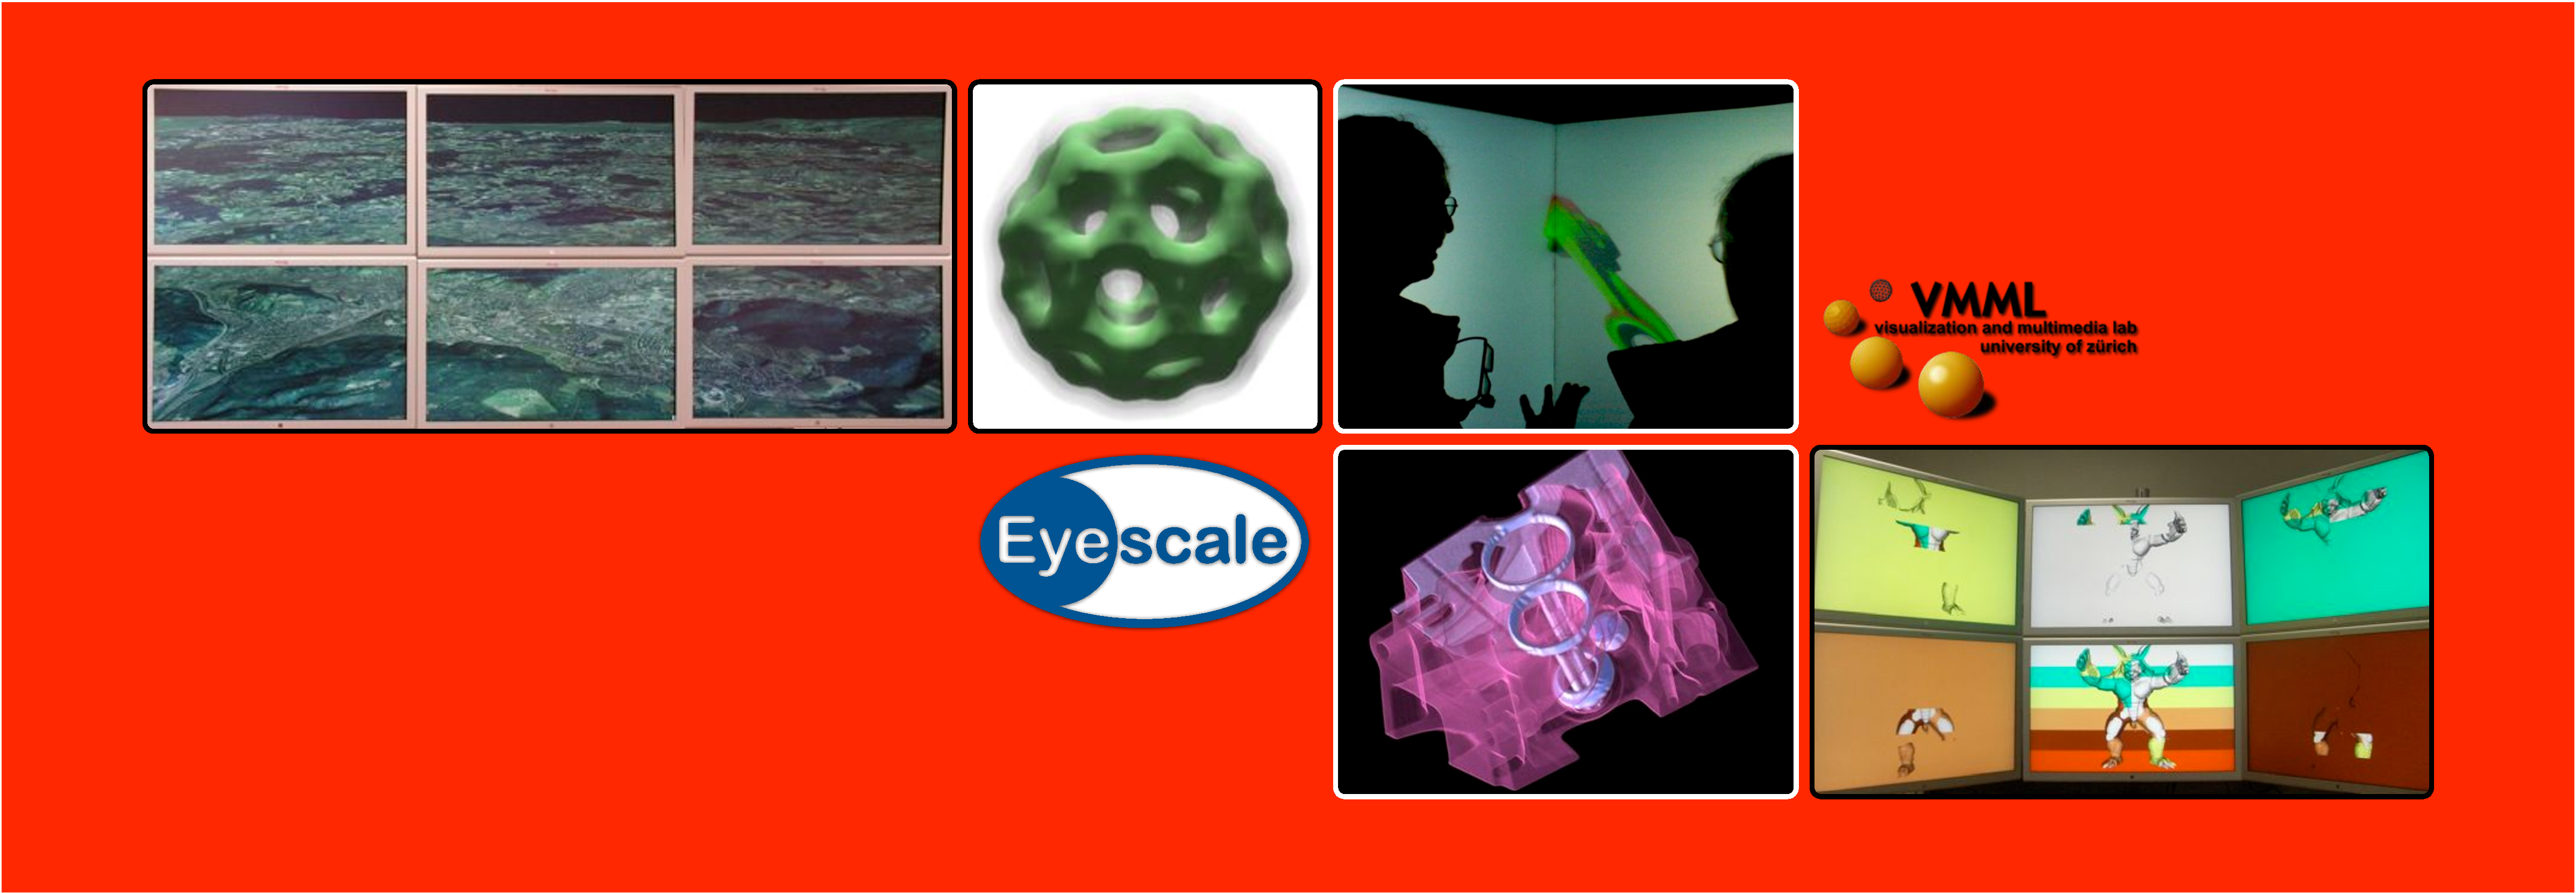
\includegraphics[width=22cm]{images/teaser.pdf}
  \end{figure}
  \vspace{1cm}
%  \textbf{RELEASE CANDIDATE}\\[\medskipamount]
  Version 1.3.9 for Equalizer 0.5.4+svn\\[\medskipamount]
  \today
}

\newcommand{\tm}{\texttrademark~}
\newcommand{\rc}{\raise 1ex\hbox{{\tiny\textregistered}}~}
\newcommand{\fig}[1]{Figure~\ref{#1}}
\newcommand{\sref}[1]{Section~\ref{#1}}
\newcommand{\aref}[1]{Appendix~\ref{#1}}
\newcommand{\link}[1]{\htmladdnormallink{#1}{#1}}

% suppress  single floating lines on top (widow) and bottom(club)
%  10000 is infinity
%  tradeoff: maybe underfull vboxes
\clubpenalty=10000
\widowpenalty=10000 

\begin{document}

\maketitle
\vfill
\lstset{language=C++}

\thispagestyle{empty}
\maketitle

\clearpage

\thispagestyle{empty}
\section*{Equalizer 0.5 Programming Guide}
\subsection*{Contributors}

Written by Stefan Eilemann.\\
Engineering contributions by Maxim Makhinya, Jonas B\"osch, Christian
Marten and Patrick Bouchaud.

\subsection*{Copyright}

\textcopyright 2007-2008 Eyescale Software GmbH. All rights reserved. No
permission is granted to copy, distribute, or create derivative works
from the contents of this electronic documentation in any manner, in
whole or in part, without the prior written permission of Eyescale
Software GmbH.

\subsection*{Trademarks and Attributions}

OpenGL is a registered trademark, OpenGL Multipipe is a trademark of
Silicon Graphics, Inc. Linux is a registered trademark of Linus
Torvalds.  Mac OS is a trademark of Apple Inc. CAVELib is a registered
trademark of the University of Illinois. The CAVE is a registered
trademark of the Board of Trustees of the University of Illinois at
Chicago. Qt is a registered trademark of Trolltech. All other
trademarks and copyrights herein are the property of their respective
owners.

\subsection*{Feedback}

If you have comments about the content, accuracy or comprehensibility of
this programming guide, please contact
\htmladdnormallink{eile@equalizergraphics.com}
{mailto:eile@equalizergraphics.com?subject=Equalizer\%20Programming\%20Guide}.

\vfill

\subsection*{Front Page}

The images on the front page show the following Equalizer applications:
a terrain rendering application on a six-node display wall [top left], a
flow visualization application for climate research\footnote{Image
  courtesy of Computer Graphics and Multimedia Systems, University of
  Siegen}, the \textsf{eVolve} volume renderer\footnote{Data set
  courtesy of General Electric, USA} [bottom left] the \textsf{eqPly}
polygonal renderer in a three-sided CAVE [bottom center], and a six-node
sort-last database decomposition with parallel direct-send
recomposition\footnote{Data set courtesy of Stanford University Computer
  Graphics Laboratory} [bottom right].

\clearpage
\thispagestyle{empty}
\tableofcontents
\vfill{\center\begin{tabularx}{\textwidth}{|l|l|X|}
    \hline
    \bf Rev & \bf Date     & \bf Changes \\
    \hline
    1.0     & Oct 28, 2007 & Initial Version for Equalizer 0.4\\
    1.2     & Apr 15, 2008 & Version for Equalizer 0.5\\
    1.3.1   & May 02, 2008 & Add \sref{sStatistics}, improved images based on 1.2 print\\
    1.3.2   & May 05, 2008 & Add network distribution on eqPly model data\\
    1.3.3   & May 10-19, 2008 & add \aref{aFileFormat}\\
    1.3.4   & July 3, 2008 & Update \sref{sStatistics}\\
    1.3.5   & July 7, 2008 & Update after namespace naming cleanup\\
    1.3.6   & July 20, 2008 & Add accum and samples to \aref{aFileFormat}, add \sref{sDrawableConfig}\\
    1.3.7   & Aug 22, 2008 & Update \sref{sEqplyWIndow} with OSWindow changes\\
    1.3.8   & Aug 25, 2008 & Update \sref{sEventHandling} with OSWindow changes\\
    1.3.9   & Aug 29, 2008 & Update \sref{sEventHandling}: event handling cleanup\\
    \hline
  \end{tabularx}}
\thispagestyle{empty}
\clearpage

\pagenumbering{arabic}

\section{Introduction}

Equalizer provides a framework for the development of parallel OpenGL
applications. Equalizer-based applications can run from a single
shared-memory system with one or multiple graphics cards up to
large-scale graphics clusters. This Programming Guide introduces the
programming interface, often using the Equalizer example \textsf{eqPly}
as a guideline.

Equalizer is the next step in the evolution of generic parallel programming
interfaces for OpenGL-based visualization applications. Existing
solutions, such as OpenGL Multipipe SDK, Cavelib and VRJuggler,
implement a subset of concepts similar to Equalizer. In other areas,
e.g., tracking device support, they provide more functionality.

In order to adapt an application for Equalizer, the programmer
structures the source code so that the OpenGL rendering can be executed
in parallel, potentially using multiple processes for cluster-based
execution. Equalizer provides the domain-specific parallel rendering
know-how and abstracts configuration, threading, synchronization,
windowing and event handling. It is a `GLUT on steroids', providing
parallel and distributed execution, scalable rendering features and
fully customizable event handling.

If you have any question regarding Equalizer programming, this
programming guide, or other specific problems you encountered, please
direct them to the \textsf{eq-dev} mailing
list\footnote{\link{http://www.equalizergraphics.com/lists.html}}.



\section{Getting Started}


\subsection{Installing Equalizer and running \textsf{eqPly}}

Equalizer can be installed by downloading the
distribution\footnote{\link{http://www.equalizergraphics.com/downloads.html}}
and compiling the source code. After installing Equalizer, please take a
look at the Quickstart
Guide\footnote{\link{http://www.equalizergraphics.com/documents/EqualizerGuide.html}}
to get familiar with the capabilities of the \textsf{eqPly} example.

Compiling Equalizer is as simple as running \textsf{make} on Linux and
Mac OS X or building the Equalizer Visual Studio 2005 solution on
Windows. Note that on Mac OS X 10.4 (Tiger), some prerequisites have to
be installed before running \textsf{make}, as explained in
\textsf{README.Darwin}.


\subsection{Equalizer Processes}

The Equalizer architecture is based on a client-server model. The client
library exposes all functionality discussed in this document to the
programmer, and provides communication between the different Equalizer
processes.

\subsubsection{Server}
Each Equalizer server is responsible for managing one visualization
system, i.e., a shared memory system or graphics cluster.  It controls
and launches the application's rendering clients.  Currently, Equalizer
only supports one application per server, but it will provide
concurrent and efficient multi-application support in future.

\subsubsection{Application}

The application connects to an Equalizer server and receives a
configuration.  Furthermore, the application also provides its render
client, which will be controlled by the server. The application reacts
on events, updates its database and controls the rendering.

\subsubsection{Render Clients}

\begin{wrapfigure}{r}{.382\textwidth}
  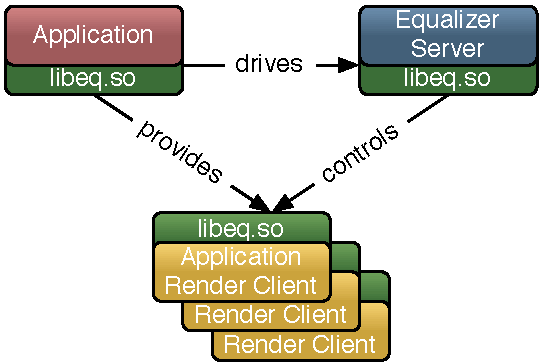
\includegraphics[width=.382\textwidth]{images/processes.pdf}
  {\caption{\small\label{fProcesses}Equalizer Processes}}
\end{wrapfigure}
The render client implements the rendering part of an application. Its
execution is passive, it has no main loop and is completely driven by
Equalizer, based on the rendering tasks received from the server. The
tasks are executed by calling the appropriate task methods (see
\sref{ssTaskMethods}) in the correct thread and context. The application
either implements the task methods with application-specific code or
uses the default methods provided by Equalizer.

The application can also be a rendering client, in which case it can
also contribute to the rendering. If it does not implement any render
client-related code, it is reduced to be the application's `master'
process without any OpenGL windows and rendering code.

The rendering client can be the same executable as the application, as
it is the case with all provided examples. When it is started as a
render client, the Equalizer initialization routine does not return and
takes over the control by calling the render client task
methods. Complex applications usually implement a separate, light-weight
rendering client.

\subsubsection{Parallel Rendering}

\begin{wrapfigure}{r}{.618\textwidth}
  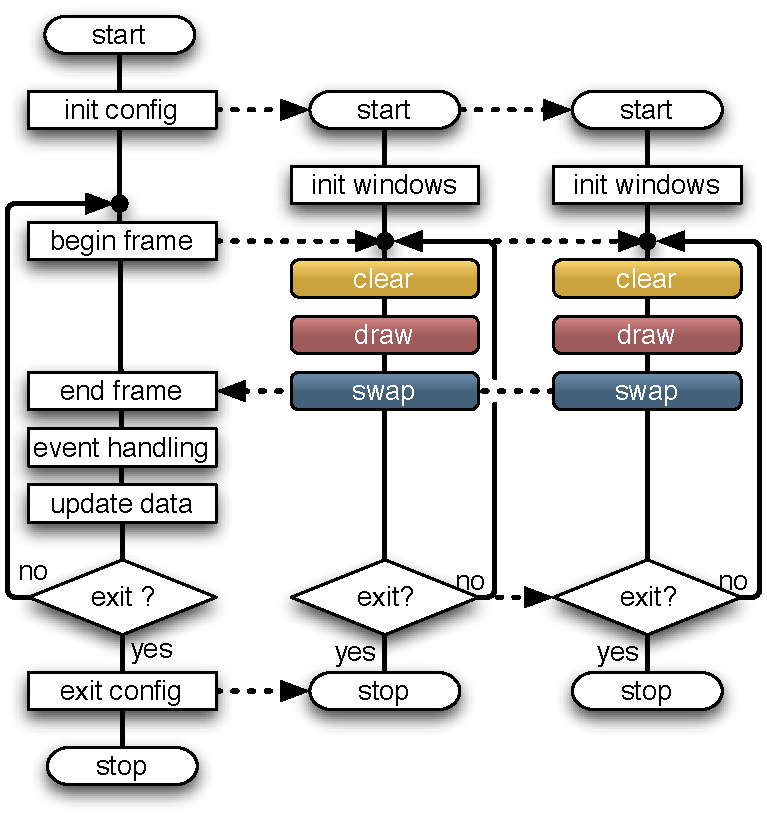
\includegraphics[width=.618\textwidth]{images/executionFlow.pdf}
  {\caption{\small\label{fExecutionFlow}Parallel Rendering}}
\end{wrapfigure}

\fig{fExecutionFlow} illustrates the basic principle of any parallel
rendering application. The typical OpenGL application, for example
GLUT-based applications, has an event loop which redraws the scene,
updates data based on received events, and eventually redraws a new
frame.

A parallel rendering application uses the same basic execution model and
extends it by separating the rendering code from the main event
loop. The rendering code is then executed in parallel on different
resources. This model is naturally followed by Equalizer, thus making
application development as easy as possible.


\section{Hello, World!}

\begin{wrapfigure}{r}{.618\textwidth}
  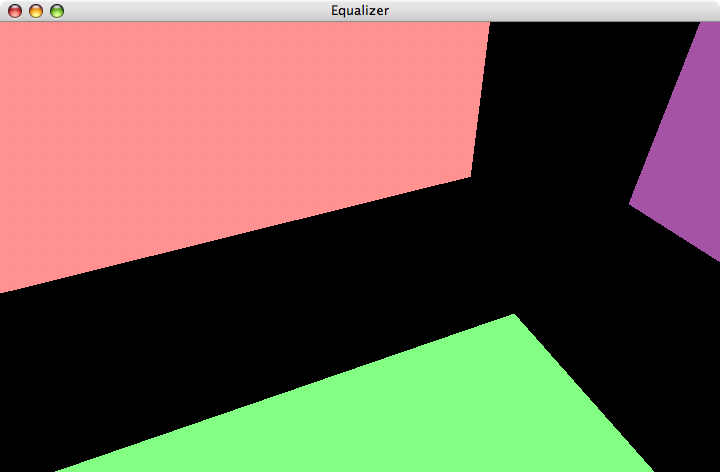
\includegraphics[width=.618\textwidth]{images/eqHello.png}
  {\caption{\small\label{fHello}Hello, World!}}
\end{wrapfigure}
The \textsf{eqHello} example is a minimal application to illustrate the
basic principle of an Equalizer application: The application developer
has to implement the rendering method \textsf{Channel::frameDraw},
similar to the \textsf{glutDisplayFunc} in GLUT applications. It can be
run as a stand-alone application from the command line.

The \textsf{eqHello} redraw function renders six colored quads, rotating
around the origin. The \textsf{frameDraw} meth\-od provided by the
\textsf{eq::Channel} can be used as a convience function to setup the
frustum and other OpenGL state. After setting up some lighting
parameters, \textsf{eqHello} rotates the scene and renders the quads
using immediate mode:

{\footnotesize\begin{lstlisting}
void Channel::frameDraw( const uint32_t spin )
{
    // setup OpenGL State
    eq::Channel::frameDraw( spin );
    
    const float lightPos[] = { 0.0f, 0.0f, 1.0f, 0.0f };
    glLightfv( GL_LIGHT0, GL_POSITION, lightPos );

    const float lightAmbient[] = { 0.2f, 0.2f, 0.2f, 1.0f };
    glLightfv( GL_LIGHT0, GL_AMBIENT, lightAmbient );

    // rotate scene around the origin
    glRotatef( static_cast< float >( spin ) * 0.5f, 1.0f, 0.5f, 0.25f );

    // render six axis-aligned colored quads around the origin
    [...]
}
\end{lstlisting}}

The \textsf{eqHello} main function sets up the communication with the
server, initializes and drives the rendering. The details of this setup
are explained in \sref{sEqPly}.


\section{Scalable Rendering}

Real-time visualization is an inherently parallel
problem. Unfortunately, different applications have different rendering
algorithms, which require different scalable rendering modes to address
the right bottlenecks. Equalizer supports the most important algorithms,
and will continue to add new ones over time to meet application
requirements.

This section gives an introduction to scalable rendering, in order to
provide some background for application developers. The scalability
modes offered by Equalizer are discussed, along with their advantages
and disadvantages. 

Choosing the right mode for the application profile is critical for
performance. Equalizer uses the concept of compounds to describe the
task decomposition and result recomposition. It allows the combination
of the different compound modes in any possible way, which allows to
address different bottlenecks in a flexible way.


\subsection{2D or Sort-First Compounds}

\begin{wrapfigure}{r}{.618\textwidth}
  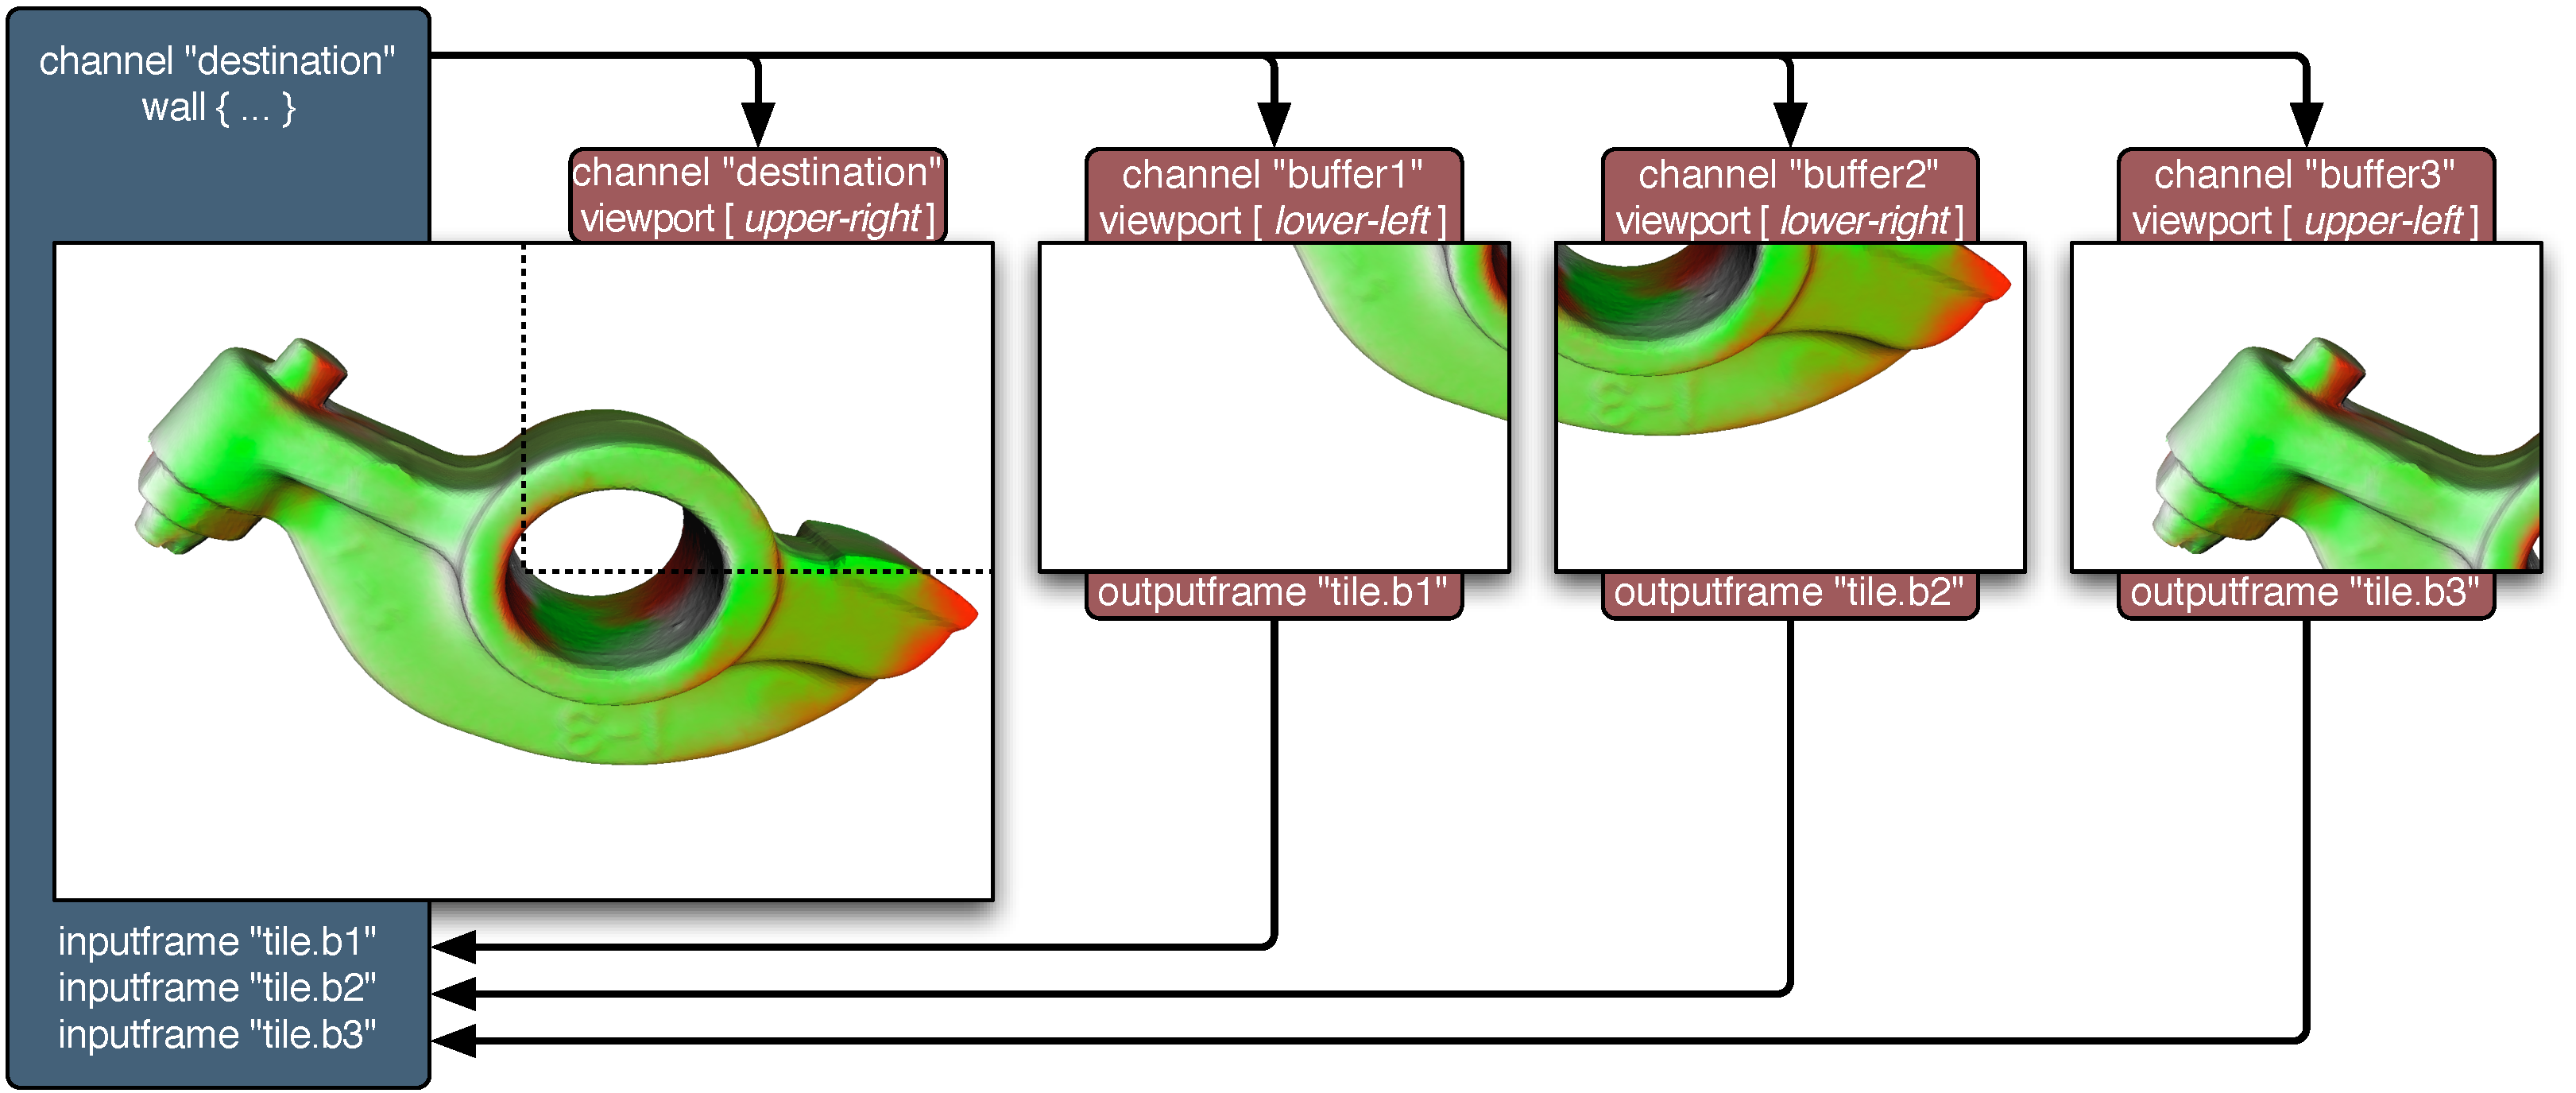
\includegraphics[width=.618\textwidth]{images/2D.pdf}
  {\caption{\small A 2D compound}}
\end{wrapfigure}
2D or sort-first decomposes the rendering in screen-space, that is, each
contributing rendering unit processes a tile of the final view. The
recomposition simply assembles the tiles side-by-side on the destination
view. 

The advantage of this mode is a low, constant IO overhead for the pixel
transfers, since only color information has to be transmitted. The upper
limit is the amount of pixel data for the destination view.

Its disadvantage is that it relies on view frustum culling to reduce the
amount of data submitted for rendering. Depending on the application
data structure, the overlap of some primitives between individual tiles
limits the scalability of this mode, typically to around eight graphics
cards. Each node has to potentially hold the full database for
rendering.

2D decompositions can be used by all types of applications, but should
be combined with DB compounds to reduce the data per node, if possible.


\subsection{DB or Sort-Last Compounds}

\begin{wrapfigure}{r}{.618\textwidth}
  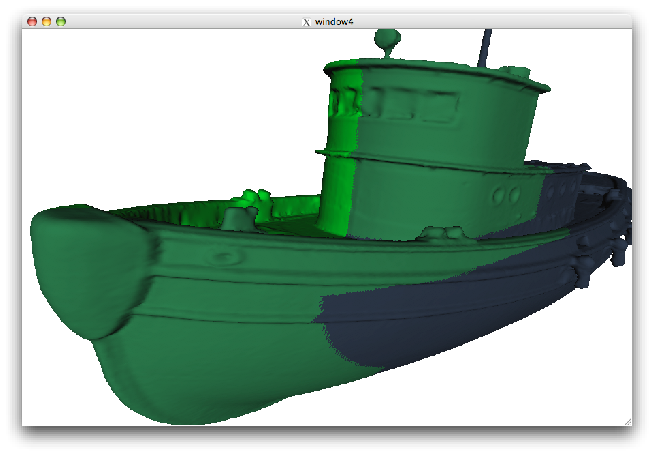
\includegraphics[width=.618\textwidth]{images/DB.pdf}
  {\caption{\small A database compound}}
\end{wrapfigure}
DB or sort-last\footnote{3D model courtesy of AVS, USA.} decomposes the
rendered database so that all rendering units process a part of the
scene in parallel.

Volume rendering applications use an ordered alpha-based blending to
composite the result image. The depth buffer information is used to
composite the individual images correctly for polygonal data. 

This mode provides very good scalability, since each rendering unit
processes only a part of the database. This allows to lower the
requirements on all parts of the rendering pipeline: main memory usage,
IO bandwidth, GPU memory usage, vertex processing and fill rate.

Unfortunately, the database recomposition has linear increasing IO
requirements for the pixel transfer. Parallel recomposition algorithms,
such as direct-send address this problem by keeping the per-node IO
constant (see \fig{fDirectSend}).

The application has to partion the database so that the rendering units
render only part of the database. Some OpenGL features do not work
correctly (anti-aliasing) or need special attention (transparency).

The best use of database compounds is to divide the data to a managable
size, and then to use other decomposition modes to achieve further
scalability. Volume rendering is one of the applications which can
profit from database compounds.


\subsection{Stereo Compounds}

\begin{wrapfigure}{r}{.618\textwidth}
  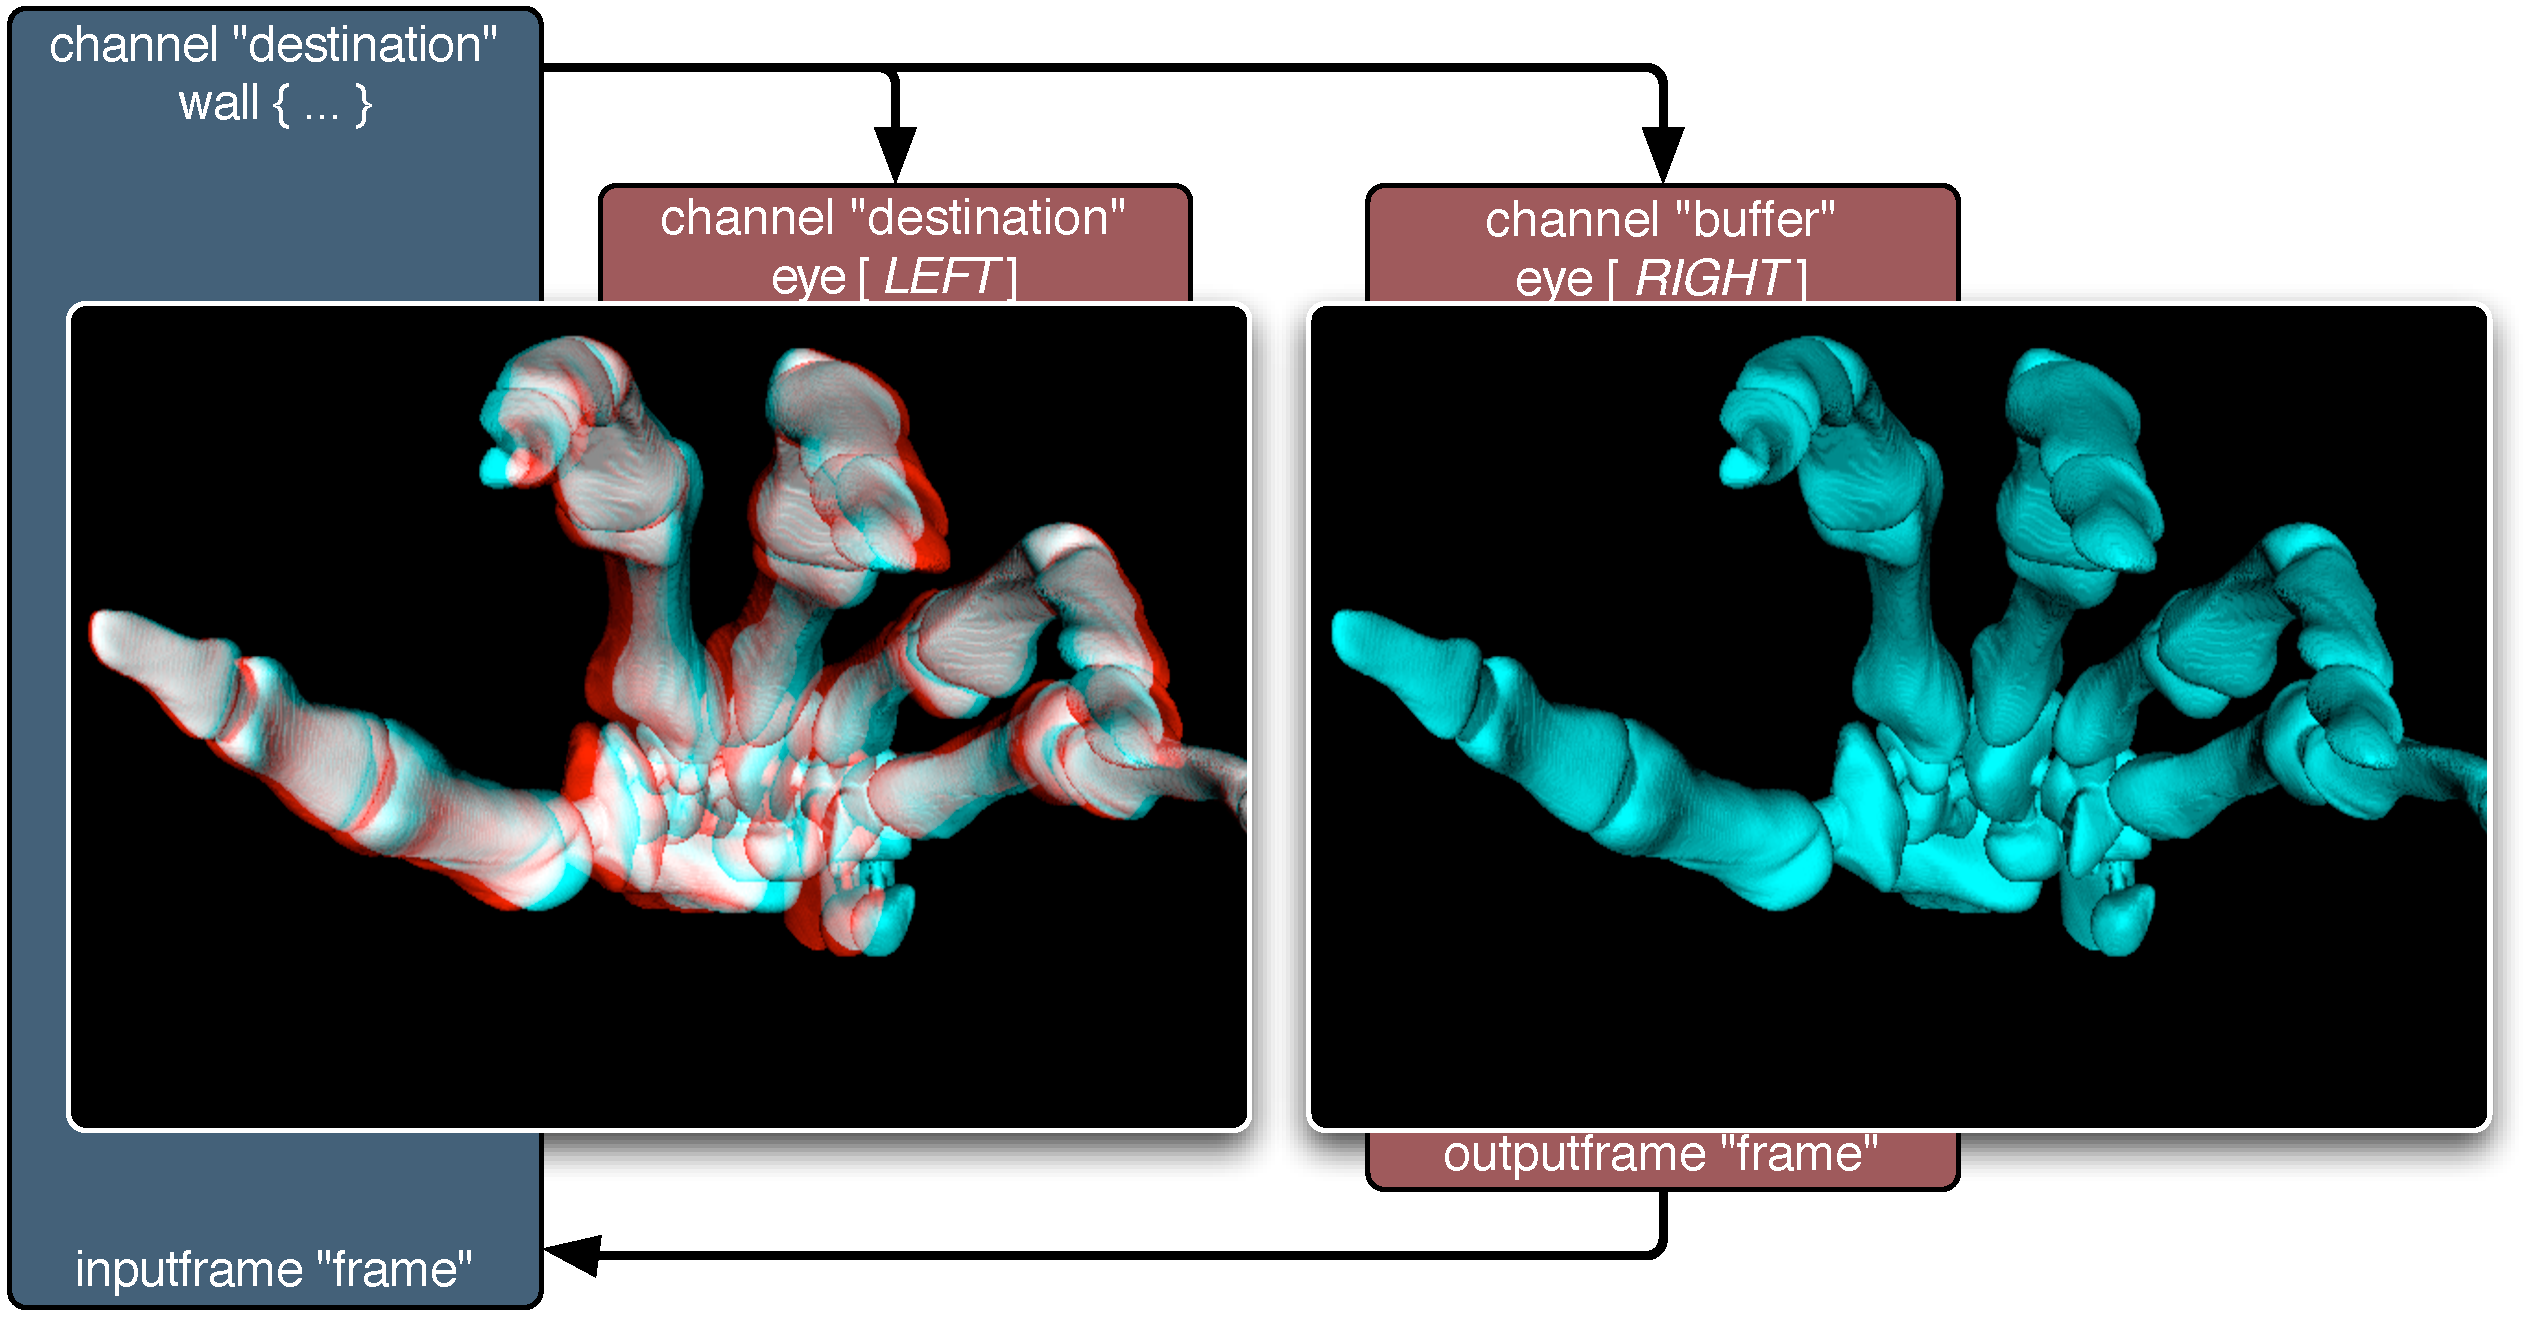
\includegraphics[width=.618\textwidth]{images/EYE.pdf}
  {\caption{\small A stereo compound}}
\end{wrapfigure}
Stereo compounds\footnote{3D model courtesy of Stereolithography Archive
  at Clemson University.} assign each eye pass to individual rendering
units. The resulting images are copied to the appropriate stereo
buffer. This modes supports a variety of stereo modes, including active
(quad-buffered) stereo, anaglyphic stereo and auto-stereo displays with
multiple eye passes.

Due to the frame consistency between the eye views, this modes scales
very well. The IO requirements for pixel transfer are small and
constant.

The number of rendering resources used by stereo compounds is limited by
the number of eye passes, typically two. 

Stereo compounds are used by all applications when rendering in stereo,
and is often combined with other modes.


\subsection{Pixel Compounds}

\begin{wrapfigure}{r}{.618\textwidth}
  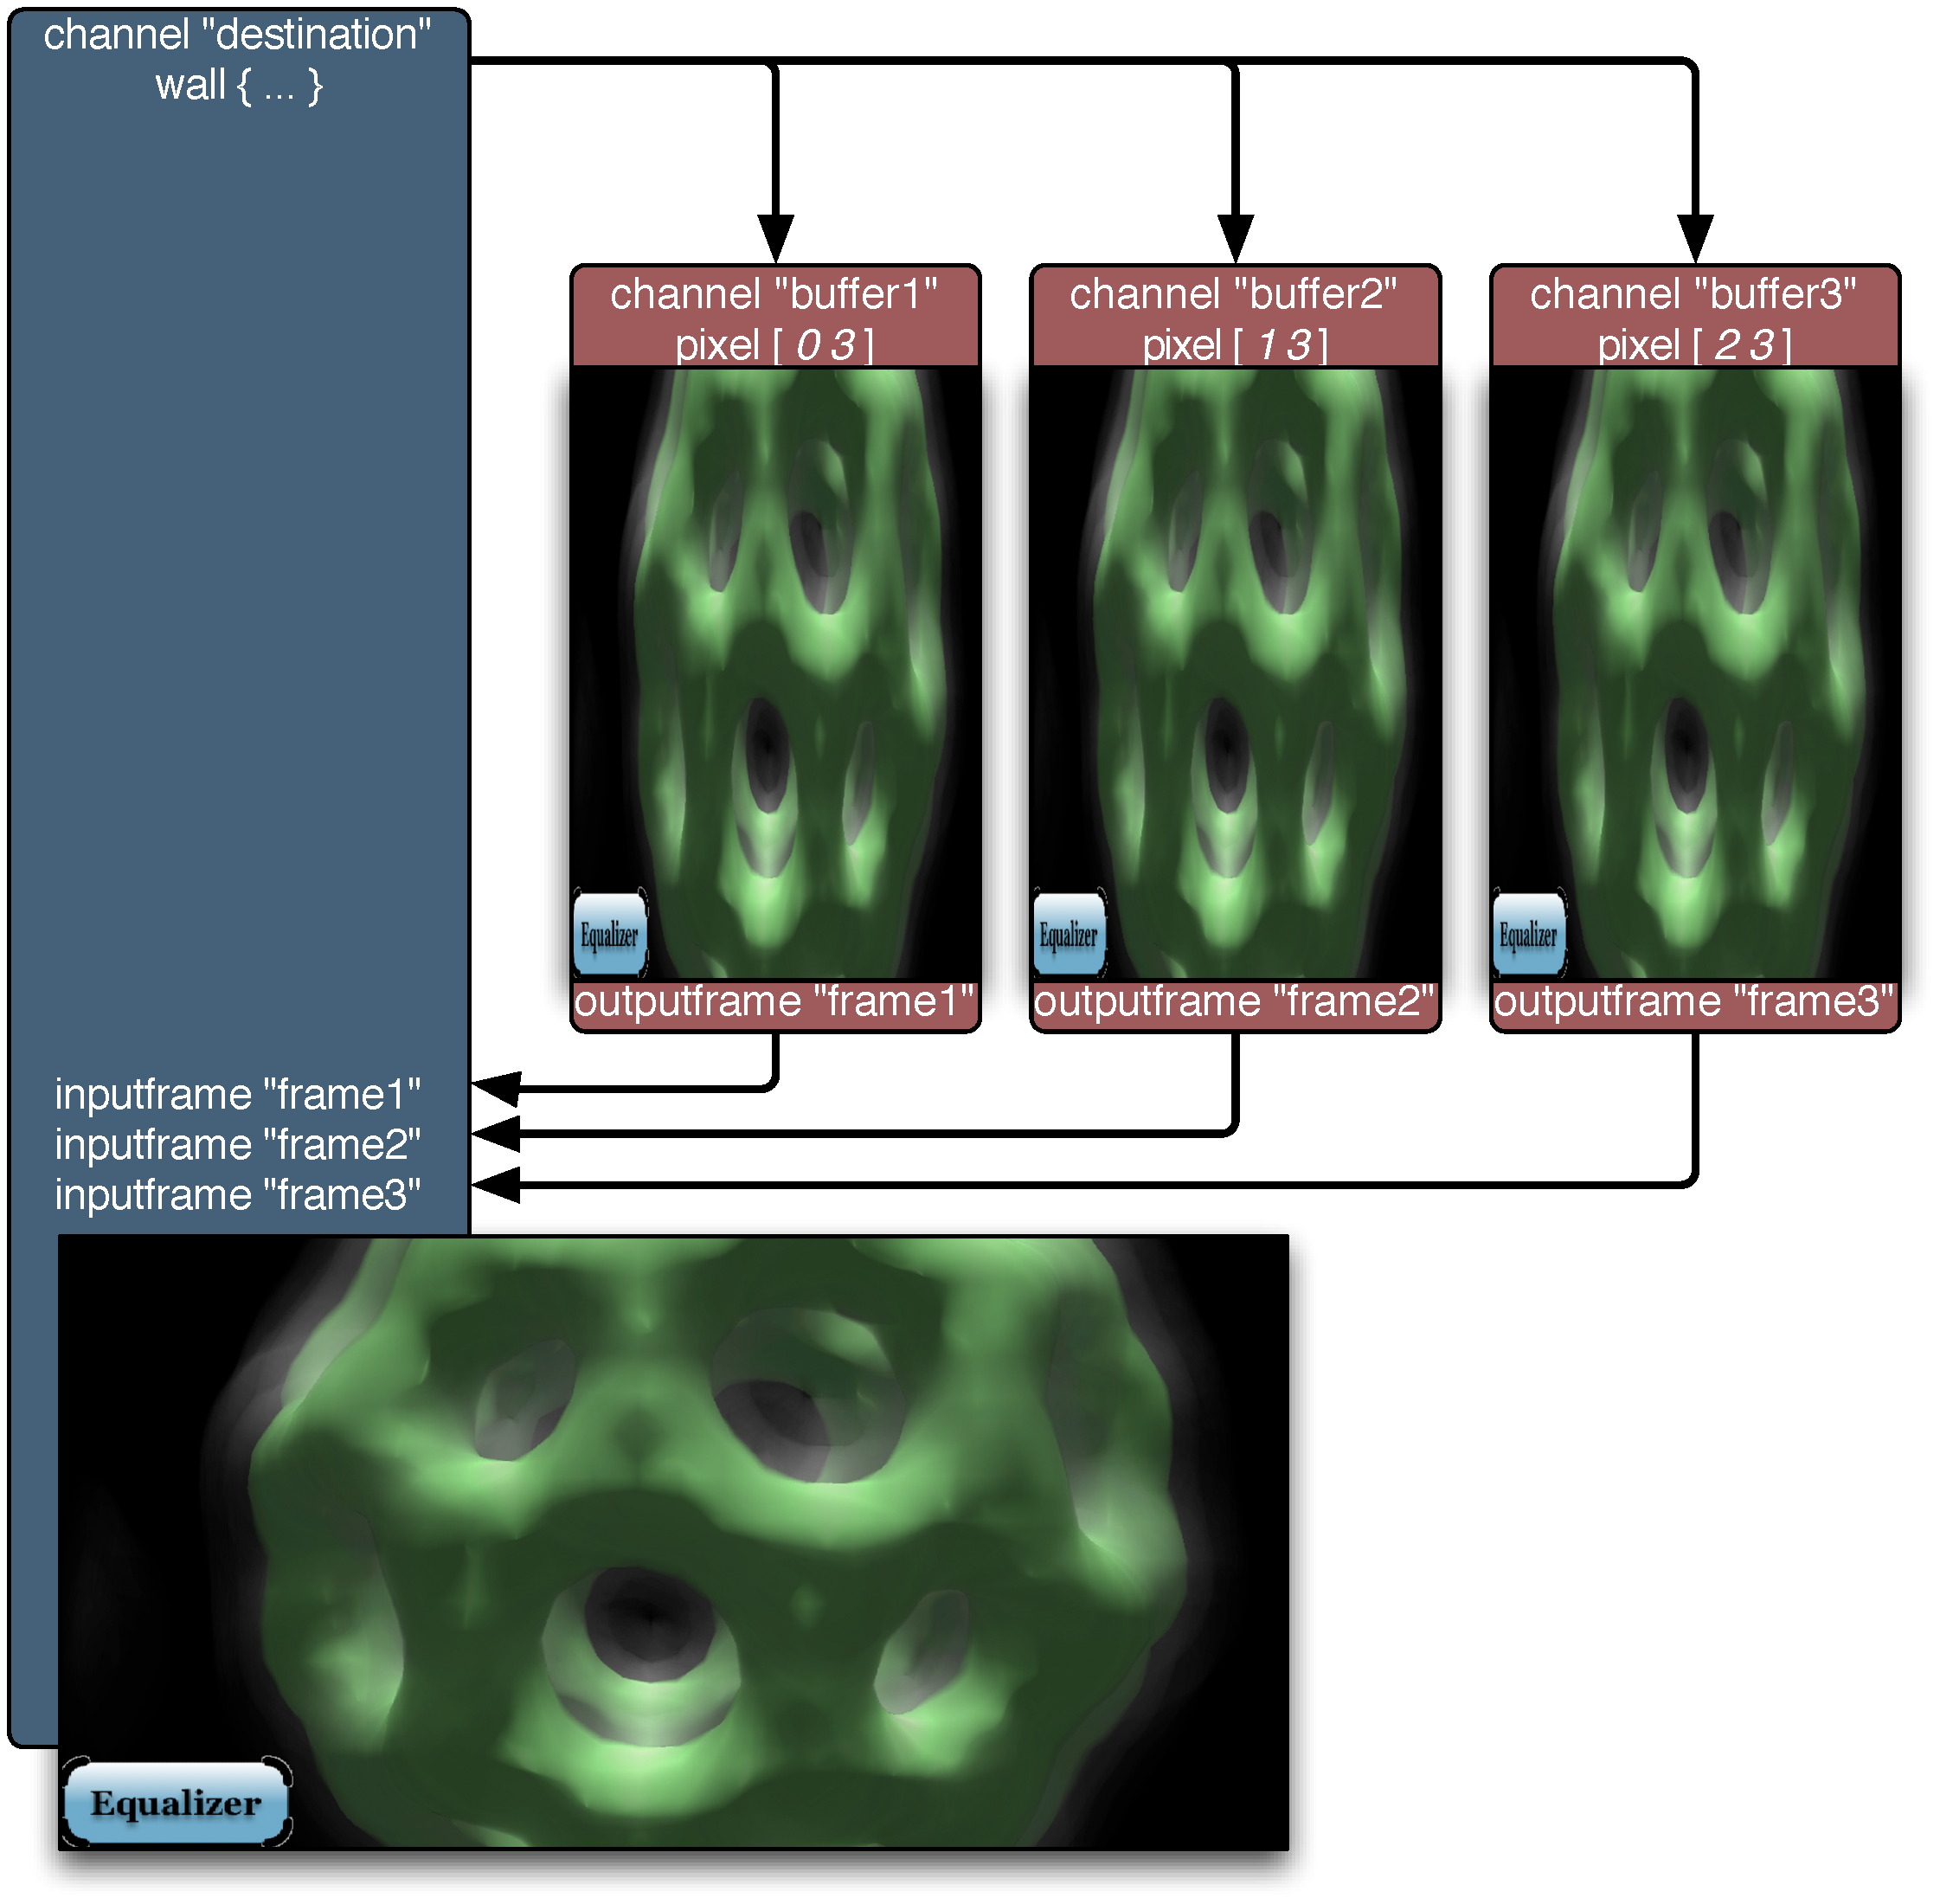
\includegraphics[width=.618\textwidth]{images/Pixel.pdf}
  {\caption{\small A pixel compound}}
\end{wrapfigure}
Pixel compounds are similar to 2D compounds. The frustra of the
source rendering units are modified so that each unit renders an evenly
distributed subset of pixels. 

As 2D compounds, pixels compounds have low, constant IO requirements for
the pixel transfers during recomposition.

Pixel compounds work well for purely fill-limited applications,
techniques like frustum culling do not reduce the rendered data for the
source rendering resources.

OpenGL functionality influenced by the raster position will not work
correctly with pixel compounds, or needs at least special
attention. Among them are: lines, points, sprites, glDrawPixels,
glBitmap, glPolygonStipple.

Pixel compounds are ideal for raytracing, which is highly fill-limited
and needs the full database for rendering anyway. Volume rendering
applications should choose this mode over 2D compounds.



\section{The Programming Interface}

Equalizer uses a C++ programming interface. The API is minimally
invasive, so Equalizer imposes only a minimal, natural execution
framework upon the application. It does not provide a scene graph, or
interfere in any other way with the application's rendering code. The
restructuring work required for Equalizer is the minimal refactoring
needed to parallelize the application for rendering.

Methods called by the application have the form \textsf{verb[Noun]},
whereas methods called by Equalizer (`Task Methods') have the form
\textsf{nounVerb}. For example, the application calls
\textsf{Config::startFrame} to render a new frame, which causes --among
other things-- \textsf{Node::frameStart} to be called in all active
render clients.


\subsection{\label{ssTaskMethods}Task Methods}

The application inherits from Equalizer classes and overrides virtual
functions to implement certain functionality, e.g., the application's
OpenGL rendering in \textsf{eq::Chan\-nel::frameDraw}. These task
methods are similar in concept to C function callbacks. The
\textsf{eqPly} section will discuss the most important task methods. A
full list can be found on the website\footnote{see
  \link{http://www.equalizergraphics.com/documents/design/taskMethods.html}}.

\subsection{\label{sExecution}Execution Model and Thread Safety}

\begin{wrapfigure}{r}{.618\textwidth}
  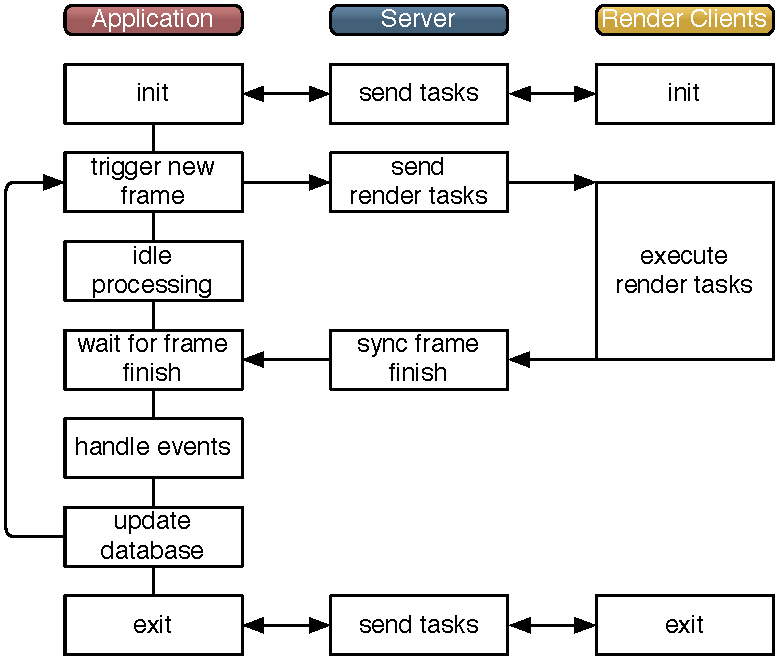
\includegraphics[width=.618\textwidth]{images/model.pdf}
  {\caption{\small\label{fModel}Simplified execution model}}
\end{wrapfigure}
Using threading correctly in OpenGL-based applications is easy with
Equalizer. Equalizer creates one rendering thread for each graphics
card. All task methods for a pipe, and therefore all OpenGL commands,
are executed from this thread. This threading model is the OpenGL
`threading model', which maintains a current context for each
thread. If structured correctly, the application rarely has to take care
of thread synchonization or protection of shared data.

The main thread is responsible for maintaining the application logic. It
reacts on user events, updates the data model and requests new frames to
be rendered. It drives the whole application, as shown in \fig{fModel}.

The rendering threads concurrently render the application's
database. The data\-base should be accessed in a read-only fashion
during rendering to avoid threading problems. This is normally the case,
for example all modern scene graphs use read-only render traversals.

All rendering threads in the configuration run asynchronously to the
application's main thread. Depending on the configuration's latency,
they can fall $n$ frames behind the last frame finished by the
application thread. A latency of one frame is usually not perceived by
the user, but can increase rendering performance substantially.

Rendering threads on a single node are by default synchronized. When a
frame is finished, all local rendering threads are done
drawing. Therefore the application can safely modify the data between
the end of a frame and the beginning of a new frame. Furthermore, only
one instance of the application data has to be maintained within a
process since all rendering threads are guaranteed to draw the same frame.

This per-node frame synchronization does not inhibit latency across
rendering nodes. Furthermore, advanced rendering software which
multi-buffers the dynamic parts of the database can disable the per-node
frame synchronization, as explained in \sref{sNodeFrame}. Some scene
graphs for example do implement multi-buffered data, and can profit from
relaxing the frame synchronization.



\subsection{\label{sConfig}Config}

The \textsf{eq::Config} represents the current configuration of the
application. The configuration is the session in which all render
clients are registered. A configuration consists of the description of
the rendering resources and the usage description for these resources.

The rendering resources are represented in a hierarchical tree structure
which corresponds to the physical and logical resources found in a 3D
rendering environment. 

The resource usage is configured using a compound tree, which is a
hierarchical representation of the rendering decomposition and
recomposition across the resources. It is explained in \sref{sCompounds}.

\begin{figure}[ht!]\center
  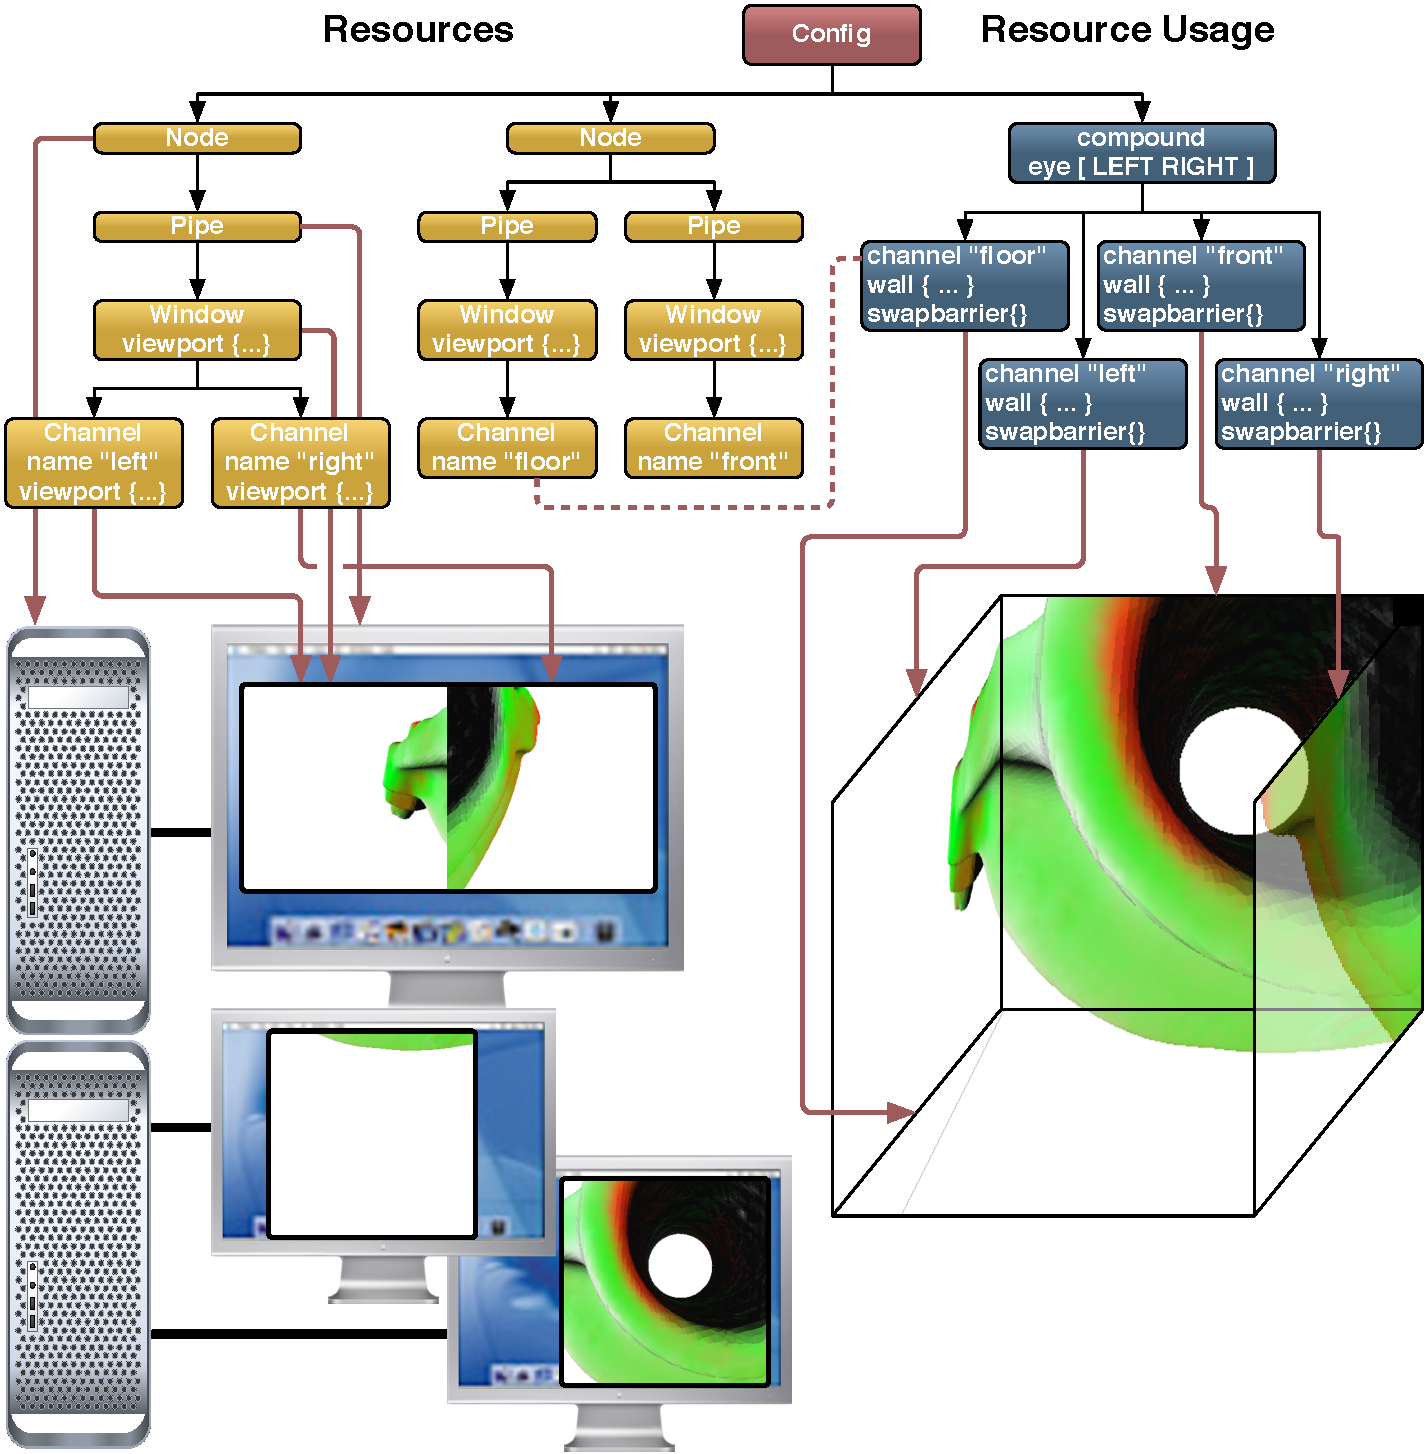
\includegraphics[width=\textwidth]{images/cave.pdf}
  {\caption{\small\label{fConfig}An example configuration}}
\end{figure}

\fig{fConfig} shows an example configuration for a four-side
CAVE, running on two machines (nodes) using three graphics
cards (pipes) with one window each to render to the four output channels
connected to the projectors for each of the walls. The compound
description is only used by the server to compute the rendering
tasks. The application is not aware of compounds, and does not need to
concern itself with the parallel rendering logics of a configuration.

For testing and development purposes it is possible to use multiple
instances for one resource, e.g. to run multiple render client nodes on
one computer. For optimal performance during deployment, one node and
pipe should be used for each computer and graphics card, respectively.

\subsubsection{Node}

The \textsf{eq::Node} class is the representation of a single computer
in a cluster. One operating system process of the render client will be
used for each node. Each configuration might also use an application
node, in which case the application process is also used for
rendering. All node-specific task methods are executed from the main
application thread.

\subsubsection{Pipe}

The \textsf{eq::Pipe} class is the abstraction of a graphics card (GPU).
In the current implementation it is also one operating system
thread. Non-threaded pipes are supported for integrating with
thread-unsafe libraries, but have various performance caveats. All pipe,
window and channel task methods are executed from the pipe's thread, or
in the case of non-threaded pipes from the main application
thread\footnote{see
  \link{http://www.equalizergraphics.com/documents/design/nonthreaded.html}}.

Further versions of Equalizer might introduce threaded windows, where
all window-related task methods are executed in a separate operating
system thread.

\subsubsection{Window}

The \textsf{eq::Window} class encapsulates a drawable and an OpenGL
context. The drawable can be an on-screen window or an off-screen
PBuffer. Framebuffer object (FBO) support will be implement by a later
version of Equalizer. The window uses an \textsf{eq::OSWindow}, which
abstracts and manages window-system-specific handles to the drawable and
context, e.g., an X11 window \textsf{XID} and \textsf{GLXContext} for
the glX window system.

\subsubsection{Channel}

The \textsf{eq::Channel} class is the abstraction of an OpenGL viewport
within its parent window. It is the entity executing the actual
rendering. The channel's viewport is overwritten when it is rendering
for another channel during scalable rendering.


\subsection{\label{sCompounds}Compounds}

Usage of the rendering resources is configured using a compound
tree. Although the API does not currently expose compounds, the basic
design behind compounds is explained here for a better understanding of
the Equalizer architecture. Further information on the configuration of
compounds can be found on the Equalizer website\footnote{see
  \link{http://www.equalizergraphics.com/documents/design/compounds.html}}.

\subsubsection{Compound Channels}
Each compound has a channel, which is used by the compound to execute
the rendering tasks. One channel might be used by multiple
compounds. Unused channels, windows, pipes and nodes are not
instantiated during config initialization. The rendering tasks for the
channels are computed by the server and send to the appropriate render
client nodes at the beginning of each frame.

\subsubsection{Frustum}
Compounds have a frustum description to define the physical layout of
the display environment. 

\begin{wrapfigure}{r}{.618\textwidth}
  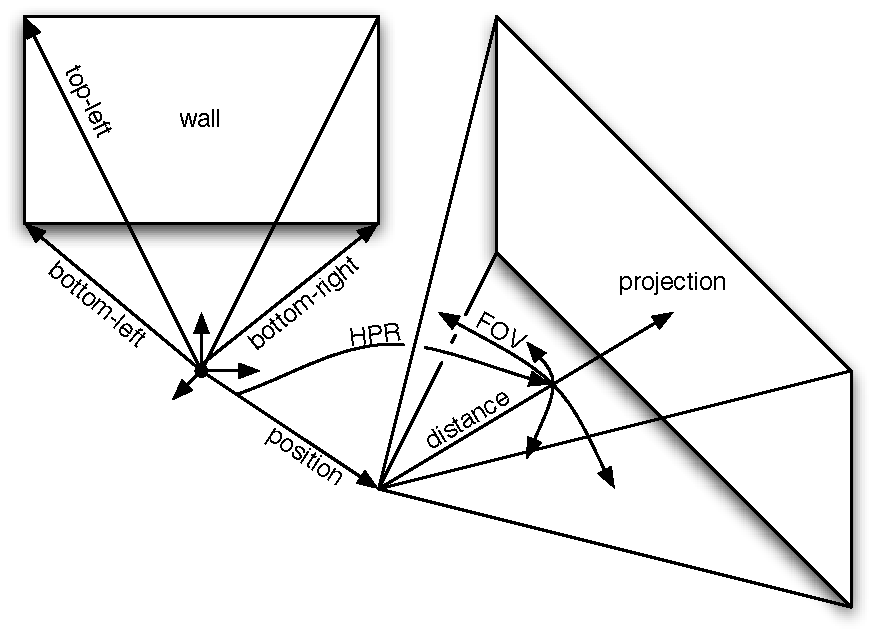
\includegraphics[width=.618\textwidth]{images/frustra.pdf}
  {\caption{\small\label{fFrustra}Wall and projection parameters}}
\end{wrapfigure}
The frustum description is inherited by the children, therefore the
frustum is typically defined on the top-most compound. 

The frustrum can be specified as a wall or projection description. 

A wall is completely defined by the bottom-left, bottom-right and
top-left coordinates relative to the origin. 

The projection is defined by the position and head-pitch-roll
orientation of the projector, as well as the horizontal and vertical
field-of-view and distance of the projection wall. 

\fig{fFrustra} illustrates the wall and projection frustum parameters.

\subsubsection{Compound Classification}
The channels of the leaf compounds in the compound tree are designated
as source channels. The top-most channel in the tree is the destination
channel. Only source channels execute the draw task. All channels in a
compound tree work for the destination channel. The destination channel
defines the 2D pixel viewport rendered by all leaf compounds. The
destination channel and pixel viewport can not be overridden by child
compounds.

\subsubsection{Decomposition - Attributes}
Compounds have attributes which configure the decomposition of the
destination's channel viewport, frustum and database. A
\textsf{viewport} decomposes the destination channel and frustum in
screen space. A \textsf{range} tells the application to render a part of
its database, and an \textsf{eye} rendering pass can selectively render
different stereo passes. A \textsf{pixel} parameter adapts the frustum
so that the source channel renders every n$th$ line out of m
lines. Setting one or multiple attributes causes the parent's view to be
decomposed accordingly. Attributes are cumulative, that is, intermediate
compound attributes affect and therefore decompose the rendering of all
their children.

\subsubsection{Recomposition - Frames}
Compounds use output and input frames to configure the recomposition of
the resulting pixel data from the source channels. An output frame
connects to an input frame of the same name. The selected frame buffer
data is transported from the output channel to the input channel. The
assembly routine of the input channel will block on the availability of
the output frame. This composition process is extensively described in
\sref{sCompositing}. Frame names are only valid within the compound
tree, that is, an output frame from one compound tree can not be used as
an input frame of another compound tree.

\subsubsection{Synchronization - Swapbarrier}
Compounds may have a swapbarrier to synchronize the buffer swap of
multiple channels. Windows with a swapbarrier of the same name enter a
barrier before executing the swap buffer task. Before entering the
barrier, \textsf{Window::finish} is called to ensure that all OpenGL
commands have been executed.

Note that this software swap barrier is not accurate enough for
edge-blended projection system. Such installations typically use a
hardware synchronization, e.g., nVidia G-Sync cards. It is however
sufficient for display walls made out of LCD's.

Swapbarrier names are only valid within the compound tree, that is, a
compound from one compound tree can not be synchronized with a compound
from another compound tree.

\section{\label{sEqPly}The eqPly polygonal renderer}

In this section the source code of \textsf{eqPly} is explained in
detail, and relevant design decisions, caveats and other remarks are
raised.

The \textsf{eqPly} example is shipped with the Equalizer distribution
and serves as a reference implementation of an Equalizer-based
application of medium complexity. It focuses on the example usage of
core Equalizer features, not on rendering features or visual quality.

\begin{figure}[ht!]\center
  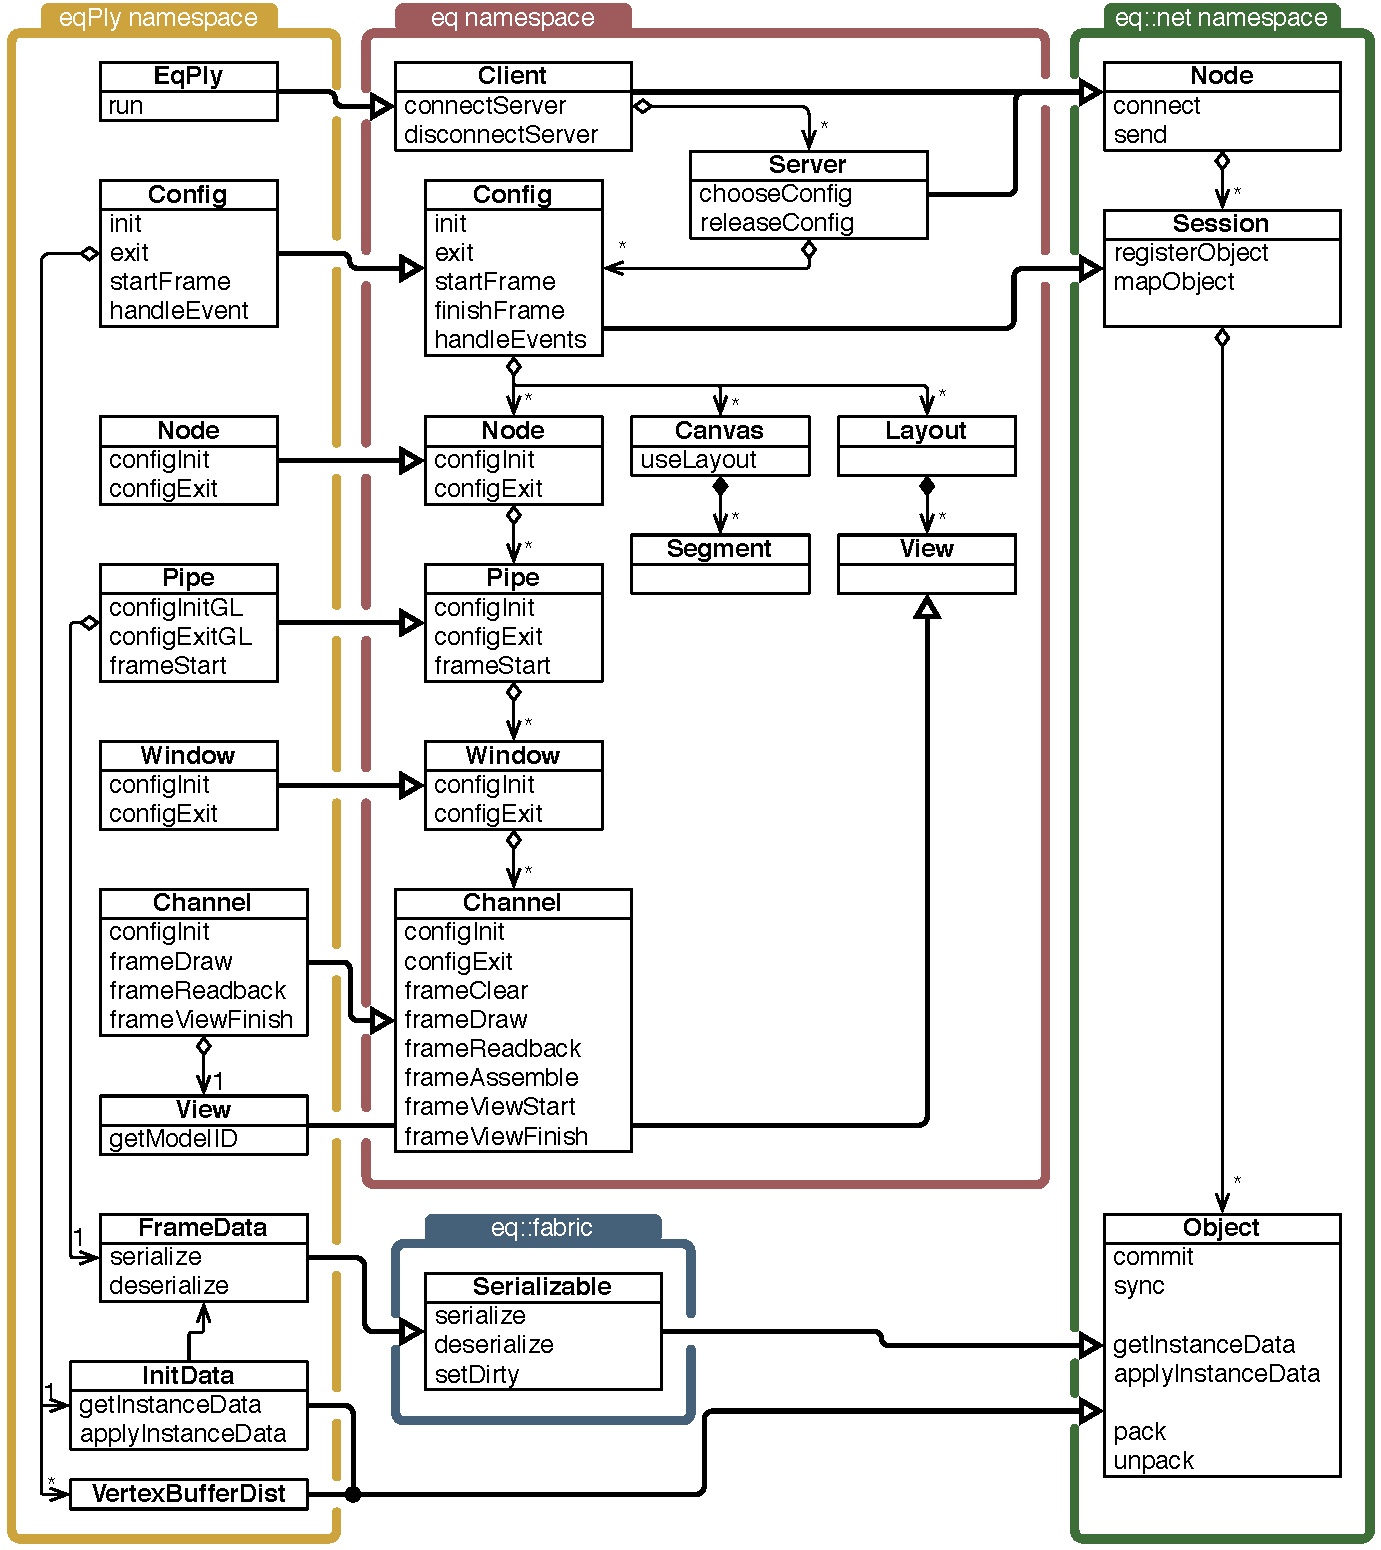
\includegraphics[width=\textwidth]{images/uml}
  {\caption{\small\label{fUml}UML diagram of significant Equalizer and
      eqPly classes and task methods.}}
\end{figure}

All classes in the example are in the \textsf{eqPly} namespace to avoid
type name ambiguities, in particular for the \textsf{Window} class which
is frequently used as a type in the global namespace by windowing
systems. \fig{fUml} shows how the most important Equalizer classes are
used through inheritance by the \textsf{eqPly} example.

The \textsf{eqPly} classes fall into two categories: Subclasses of the
rendering entities introduced in \sref{sConfig}, and two other classes
for distributing data. The function and typical usage for each of the
rendering entities is discussed in this section. 

The distributed data classes are helper classes based on
\textsf{eq::net::Object}. They illustrate the typical usage of distributed
objects for static as well as dynamic, frame-specific data.


\subsection{The main Function}

The main function starts off with parsing the command line into the
\textsf{LocalInitData} data structure. A part of it, the base class
\textsf{InitData}, will be distributed to all render client nodes. The
command line parsing is done by the \textsf{LocalInitData} class, which
is discussed in \sref{sInitData}:

{\footnotesize\begin{lstlisting}
int main( int argc, char** argv )
{
    // 1. parse arguments
    eqPly::LocalInitData initData;
    initData.parseArguments( argc, argv );
\end{lstlisting}}

The second step is to initialize the Equalizer library. The
initialization function of Equalizer also parses the command line, which
is used to set certain default values based on Equalizer-specific
options\footnote{Equalizer-specific options always start with -\,-eq-},
e.g., the default server address. Furthermore, a \textsf{NodeFactory} is
provided. The \textsf{EQERROR} macro, and its counterparts
\textsf{EQWARN}, \textsf{EQINFO} and \textsf{EQVERB} allow selective
debugging outputs with various logging levels:

{\footnotesize\begin{lstlisting}
    // 2. Equalizer initialization
    NodeFactory nodeFactory;
    if( !eq::init( argc, argv, &nodeFactory ))
    {
        EQERROR << "Equalizer init failed" << endl;
        return EXIT_FAILURE;
    }
\end{lstlisting}}%>>

The node factory is used by Equalizer to create the object instances of
the configured rendering entities. Each of the classes inherits from the
same type provided by Equalizer in the \textsf{eq} namespace. The
provided \textsf{eq::NodeFactory} base class instantiates 'plain'
Equalizer objects, thus making it possible to selectively subclass
individual entity types, as it is done by \textsf{eqHello}. For each
rendering resources used in the configuration, one C++ object will be
created during initialization. Config, node and pipe objects are created and
destroyed in the node thread, whereas window and channel objects are
created and destroyed in the pipe thread:

{\footnotesize\begin{lstlisting}
class NodeFactory : public eq::NodeFactory
{
public:
    virtual eq::Config*  createConfig()  
        { return new eqPly::Config; }
    virtual eq::Node*    createNode( eq::Config* parent )  
        { return new eqPly::Node( parent ); }
    virtual eq::Pipe*    createPipe( eq::Node* parent )
        { return new eqPly::Pipe( parent ); }
    virtual eq::Window*  createWindow( eq::Pipe* parent )
        { return new eqPly::Window( parent ); }
    virtual eq::Channel* createChannel( eq::Window* parent )
        { return new eqPly::Channel( parent ); }
};
\end{lstlisting}}

The third step is to create an instance of the application and to
initialize it locally. The application is an \textsf{eq::Client}, which
in turn is an \textsf{eq::net::Node}. The underlying network layer in
Equalizer is a peer-to-peer network of \textsf{eq::net::Node}s. The
application programmer does not usually have to be aware of the classes
in the \textsf{eq::net} namespace, but both the \textsf{eq::Client} and
the server are \textsf{eq::net::Node}s. 

The local initialization of a node creates a local listening socket,
which allows the \textsf{eq::Client} to communicate over the network
with other nodes, such as the server and the rendering clients.

{\footnotesize\begin{lstlisting}
    // 3. initialization of local client node
    RefPtr< eqPly::Application > client = new eqPly::Application( initData );
    if( !client->initLocal( argc, argv ))
    {
        EQERROR << "Can't init client" << endl;
        eq::exit();
        return EXIT_FAILURE;
    }
\end{lstlisting}}%>>

Finally everything is set up, and the \textsf{eqPly} application is executed:

{\footnotesize\begin{lstlisting}
    // 4. run client
    const int ret = client->run();
\end{lstlisting}}

After the application has finished, it is de-initialized and the
\textsf{main} function returns:

{\footnotesize\begin{lstlisting}
    // 5. cleanup and exit
    client->exitLocal();
    client = 0;

    eq::exit();
    return ret;
}
\end{lstlisting}}


\subsection{Application}

In the case of \textsf{eqPly}, the application is also the render
client. The \textsf{eqPly} executable has three run-time behaviours:

\begin{enumerate}
\item \textbf{Application}: The executable started by the user, the
  controlling entity in the rendering session.
\item \textbf{Auto-launched render client}: The typical render client,
  started by the server. The server starts the executable with special
  parameters, which cause \textsf{Client::initLocal} to never
  return. During exit, the server terminates the process. By default,
  the server starts the render client using \textsf{ssh}.
\item \textbf{Resident render client}: Manually pre-started render
  client, listening on a specified port for server commands. This mode
  is selected using the command-line option \textsf{--eq-client} and
  potentially \textsf{--eq-listen \textless address\textgreater} and
  \textsf{-r}\footnote{see
    \link{http://www.equalizergraphics.com/documents/design/residentNodes.html}}.
\end{enumerate}

\subsubsection{Main Loop}

The application's main loop starts by connecting the application to an
Equalizer server. The command line parameter \textsf{--eq-server}
explicitly specifies a server address. If no server was specified,
\textsf{Client::connectServer} tries first to connect to a server on the
local machine using the default port. If that fails, it will create
a server running within the application process with a default
one-channel configuration\footnote{see
  \link{http://www.equalizergraphics.com/documents/design/standalone.html}}.

{\footnotesize\begin{lstlisting}
int Application::run()
{
    // 1. connect to server
    RefPtr<eq::Server> server = new eq::Server;
    if( !connectServer( server ))
    {
        EQERROR << "Can't open server" << endl;
        return EXIT_FAILURE;
    }
\end{lstlisting}}%>>

The second step is to ask the server for a configuration. The
\textsf{ConfigParams} are a placeholder for later Equalizer
implementations to provide additional hints and information to the
server for choosing the configuration. The configuration chosen by the
server is created locally using
\textsf{NodeFactory::createConfig}. Therefore it is of type
\textsf{eqPly::Config}, but the return value is \textsf{eq::Config},
making the cast necessary:

{\footnotesize\begin{lstlisting}
    // 2. choose config
    eq::ConfigParams configParams;
    Config* config = static_cast<Config*>(server->chooseConfig( configParams ));

    if( !config )
    {
        EQERROR << "No matching config on server" << endl;
        disconnectServer( server );
        return EXIT_FAILURE;
    }
\end{lstlisting}}%>>

Finally it is time to initialize the configuration. For statistics, the
time for this operation is measured and printed. During initialization
the server launches and connects all render client nodes, and calls the
appropriate initialization task methods, as explained in later
sections. \textsf{Config::init} returns after all nodes, pipes,
windows and channels are initialized. It returns \textsf{true} only if
all initialization task methods were successful.

The \textsf{EQLOG} macro allows topic-specific logging. The numeric
topic values are specified in the respective \textsf{log.h} header
files, and logging for various topics is enabled using the environment
variable \textsf{EQ\_LOG\_TOPICS}:

{\footnotesize\begin{lstlisting}
    // 3. init config
    eq::base::Clock clock;

    config->setInitData( _initData );
    if( !config->init( ))
    {
        EQERROR << "Config initialization failed: " 
                << config->getErrorMessage() << endl;
        server->releaseConfig( config );
        disconnectServer( server );
        return EXIT_FAILURE;
    }

    EQLOG( eq::LOG_CUSTOM ) << "Config init took " << clock.getTimef() << " ms"
                            << endl;
\end{lstlisting}}%>>

When the configuration was successfully initialized, the main rendering
loop is executed. It runs until the user exits the
configuration, or when a maximum number of frames has been rendered,
specified by a command-line argument. The latter is useful for
benchmarks. The \textsf{Clock} is reused for measuring the overall
performance. A new frame is started using \textsf{Config::startFrame}
and a frame is finished using \textsf{Config::finishFrame}.

When the frame is started, the server computes all rendering tasks and
sends them to the appropriate render client nodes. The render client
nodes dispatch the tasks to the correct node or pipe thread, where they
are executed in order of arrival.

\textsf{Config::finishFrame} synchronizes on the completion of the frame
\textsf{current - latency}. The latency is specified in the
configuration file, and allows several outstanding frames. This allows
overlapping execution in the node and pipe threads and minimizes idle
times. 

By default, \textsf{Config::finish\-Fra\-me} also synchronizes the
completion of all local rendering tasks for the current frame. This
facilitates porting of exising rendering codes, since the database does
not have to be multi-buffered. Applications such as \textsf{eqPly}, which
do not need this per-node frame synchronization can disable it, as
explained in \sref{sNodeFrame}.

\begin{figure}[ht!]\center
  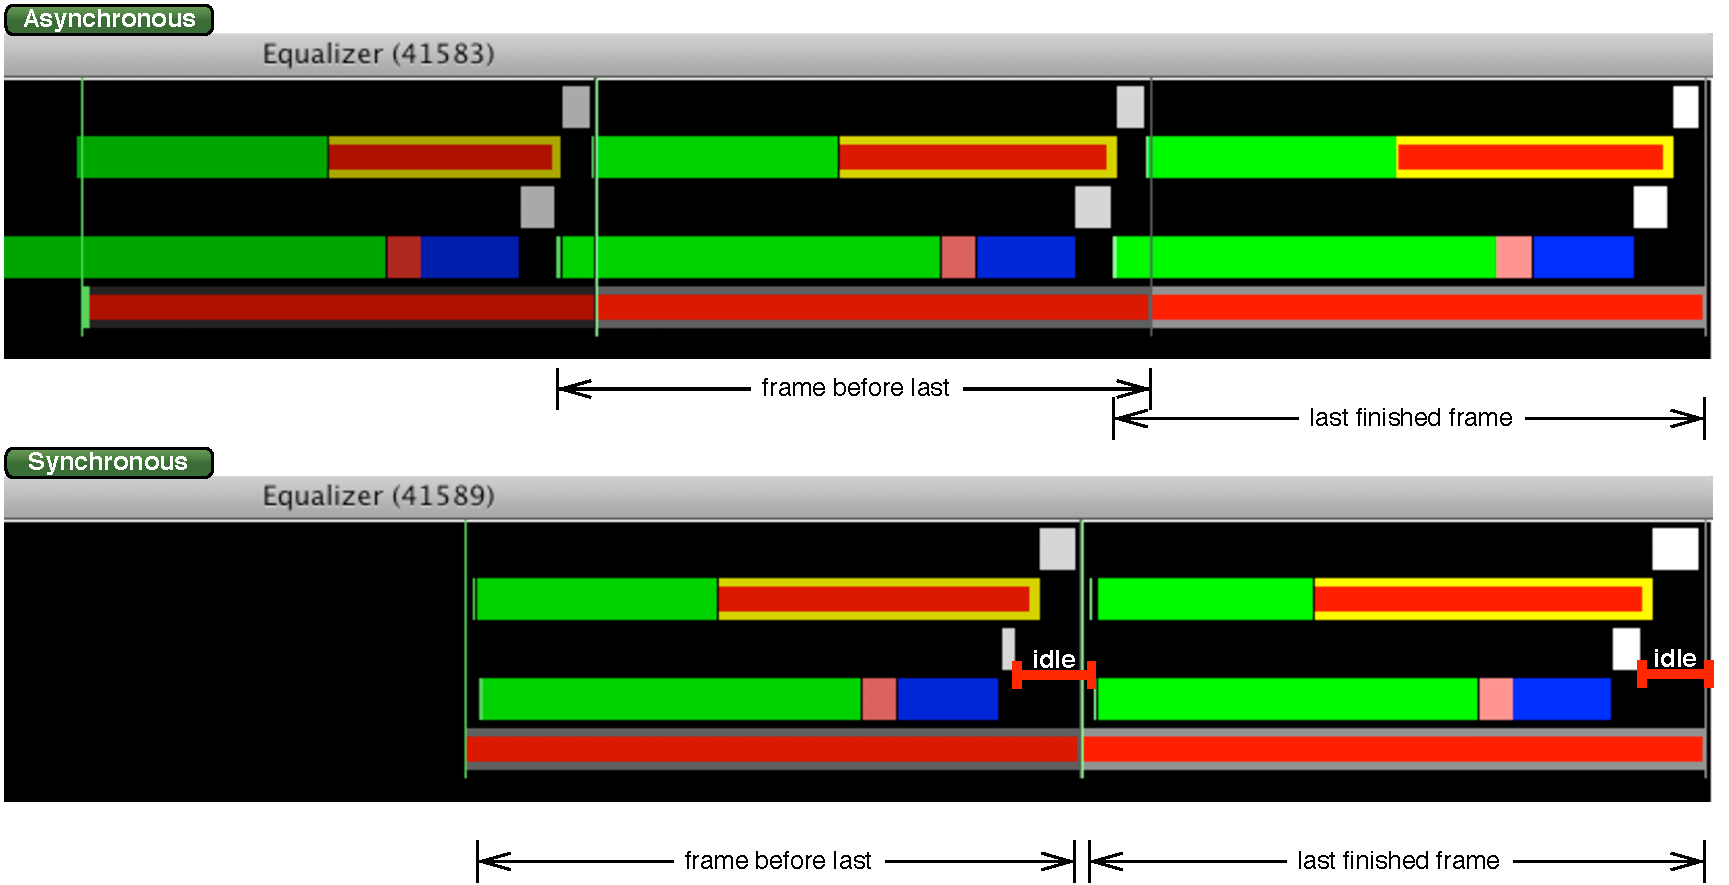
\includegraphics[width=\textwidth]{images/syncAsync}
  {\caption{\small\label{fSyncAsync}Synchronous and asynchronous execution}}
\end{figure}
\fig{fSyncAsync} shows the execution of the rendering tasks of a 2-node
2D compound without latency and with a latency of one frame. The
asynchronous execution pipelines certain rendering operations and hides
imbalances in the load distribution, resulting in an improved
framerate. With \textsf{eqPly}, a speedup of 15\% has been observed on a
five-node rendering cluster when using a latency of one frame instead of
no
latency\footnote{\link{http://www.equalizergraphics.com/scalability.html}}. A
latency of one or two frames is normally not perceived by the user.

When the main rendering loop has finished,
\textsf{Config::finishAllFrames} is called to catch up with the
latency. It returns after all outstanding frames have been rendered, and
is needed to provide an accurate measurement of the framerate:

{\footnotesize\begin{lstlisting}
    // 4. run main loop
    uint32_t maxFrames = _initData.getMaxFrames();
    
    clock.reset();
    while( config->isRunning( ) && maxFrames-- )
    {
        config->startFrame();
        // config->renderData(...);
        config->finishFrame();
    }
    const uint32_t frame = config->finishAllFrames();
    const float    time  = clock.getTimef();
    EQLOG( eq::LOG_CUSTOM ) << "Rendering took " << time << " ms (" << frame
                            << " frames @ " << ( frame / time * 1000.f)
                            << " FPS)" << endl;
\end{lstlisting}}%>>

The remainder of the application code cleans up in the reverse order of
initialization. The config is exited, released and the connection to
the server is closed:

{\footnotesize\begin{lstlisting}
    // 5. exit config
    clock.reset();
    config->exit();
    EQLOG( eq::LOG_CUSTOM ) << "Exit took " << clock.getTimef() << " ms" <<endl;

    // 6. cleanup and exit
    server->releaseConfig( config );
    if( !disconnectServer( server ))
        EQERROR << "Client::disconnectServer failed" << endl;
    server = 0;
    return EXIT_SUCCESS;
}
\end{lstlisting}}%>>

\subsubsection{Render Clients}

In the second and third use case of the \textsf{eqPly}, when the
executable is used as a render client, \textsf{Client::initLocal} never
returns. Therefore the application's main loop is never executed. In
order to keep the client resident, the \textsf{eqPly} example overrides
the client loop to keep it running beyond one configuration run:

{\footnotesize\begin{lstlisting}
bool Application::clientLoop()
{
    if( !_initData.isResident( )) // execute only one config run
        return eq::Client::clientLoop();

    // else execute client loops 'forever'
    while( true ) // TODO: implement SIGHUP handler to exit?
    {
        if( !eq::Client::clientLoop( ))
            return false;
        EQINFO << "One configuration run successfully executed" << endl;
    }
    return true;
}
\end{lstlisting}}%>>


\subsection{Distributed Objects}

Equalizer provides distributed objects which help implementing data
distribution in a cluster environment. The master version of a distributed
object is registered with a \textsf{eq::net::Session}, which assigns a
session-unique identifier to the object. Other nodes can map their
instance of the object to this identifier, thus synchronizing the
object's data with the remotely registered master version.

Distributed objects are created by subclassing from
\textsf{eq::net::Object}. Distributed objects can be static (immutable) or
dynamic. Dynamic objects are versioned.

The \textsf{eqPly} example uses static distributed objects to provide
initial data and the model to all rendering nodes, as well as a
versioned object to provide frame-specific data such as the camera
position to the rendering methods.

\subsubsection{Common Usage}

Distributed objects are addressed using session-unique identifiers,
because pointers to other objects can not be distributed directly, since
they have no meaning on remote nodes. The session with which distributed
objects are registered is normally the \textsf{eq::Config}.

The shared data entry point for the render clients is the identifier
passed by the application to \textsf{Config::init}. This identifier
typically contains the identifier of a static distributed object, and is
passed by Equalizer to all \textsf{configInit} task methods. Normally
this initial object is mapped by the render clients, and it contains
identifiers to other shared data objects.

The distributed data objects referenced by the initial data object are
often versioned objects, to keep them in sync with the rendered
frames. Similar to the initial identifier passed to
\textsf{Config::init}, an object identifier or version can be passed to
\textsf{Config::startFrame}. Equalizer will pass this identifier to all
\textsf{frameStart} task methods. In \textsf{eqPly}, the frame-specific
data, e.g., the global camera data, is versioned. The frame data
identifier is passed in the initial data, and the frame data version is
passed with each start frame request.

\subsubsection{Change Handling}

The way changes are to be handled is determined by calling
\textsf{Object::getChangeType} during the registration of the master
version of a distributed object. The change type determines the memory
footprint and the contract for calling the serialization methods. The
following change types are possible:

\begin{description}
  \item[STATIC] The object is not versioned. The instance data is
    serialized whenever a new slave instance is mapped. No additional
    data is stored.
  \item[INSTANCE] The object is versioned, and the instance and delta
    data is identical, that is, only instance data is
    serialized. Previous instance data is saved to be able to map old
    versions.
  \item[DELTA] The object is versioned, and the delta data is typically
    smaller than the instance data. Both the delta and instance data are
    serialized and saved to map old versions.
  \item[DELTA\_UNBUFFERED] The object is versioned, and delta data is
    used to update slave instances. No data is stored, and no previous
    versions can be mapped. The instance data is serialized whenever a
    new slave instance is mapped.
\end{description}

\subsubsection{\label{sInitData}InitData - a Static Distributed Object}

The \textsf{InitData} class holds a couple of parameters needed during
initialization. These parameters never change during one configuration
run, and are therefore static.

On the application side, the class \textsf{LocalInitData} subclasses
\textsf{InitData} to provide the command line parsing and to set the
default values. The render nodes only instantiate the distributed part
in \textsf{InitData}.

A static distributed object either has to provide a pointer and size to
its data using \textsf{setInstanceData}, or it has to implement
\textsf{getInstanceData} and \textsf{applyInstanceData}. The first
approach can be used if all distributed member variables are stored in
one contiguous block of memory. The second approach is used otherwise.

The \textsf{InitData} class contains a string of variable
length. Therefore it uses the second approach of manually serializing
and de-serializing its data. Serialization in \textsf{getInstanceData}
and de-serialization in \textsf{applyInstanceData} is performed by
streaming all member variable to or from the provided data
streams. Efficient buffering and data transport between nodes is
implemented in the data streams:

{\footnotesize\begin{lstlisting}
void InitData::getInstanceData( eq::net::DataOStream& os )
{
    os << _frameDataID << _modelID << _windowSystem << _useVBOs << _useGLSL
       << _invFaces ;
}

void InitData::applyInstanceData( eq::net::DataIStream& is )
{
    is >> _frameDataID >> _modelID >> _windowSystem >> _useVBOs >> _useGLSL
       >> _invFaces;

    EQASSERT( _frameDataID != EQ_ID_INVALID );
    EQINFO << "New InitData instance" << endl;
}
\end{lstlisting}}%>>

The data input and output streams perform no type checking on the data.
It is the application's responsibility to exactly match the order and
types of variables during serialization and de-serialization.

\subsubsection{FrameData - a Versioned Distributed Object}

Versioned objects have to override \textsf{getChangeType} to indicate
how they want to have changes to be handled. The current
implementation has the following characteristics:
\begin{itemize}
\item Only the master instance of the object is writable, that is,
  \textsf{eq::net::Object::com\-mit} can be called only on the master
  instance to generate a new version.
\item Slave instance versions can only be advanced, that is,
  \textsf{eq::net::Object::sync( version )} with a version smaller than
  the current version will fail.
\item Newly mapped slave instance are mapped to the oldest available
  version.
\end{itemize}

Upon \textsf{commit} the delta data from the previous version is sent to
all mapped slave instances. The data is queued on the remote node, and
is applied when the application calls \textsf{sync} to synchronize the
object to a new version. The \textsf{sync} method might block if a
version has not been committed or is still in transmission.

In addition to the instance data (de)serialization methods used to map
an object, versioned objects may implement \textsf{pack} and
\textsf{unpack} to serialize or de-serialize the changes since the last
version.

If the delta data happens to be layed out contiguously in memory,
\textsf{setDeltaData} might be used. The default implementation of
\textsf{pack} and \textsf{unpack} (de)serialize the delta data or the
instance data if no delta data has been specified.

The \textsf{eqPly} frame data is layed out in one anonymous structure in
memory. It also does not track changes since it is relatively small in
size and changes frequently. Therefore, the instance and delta data are
the same and set in the constructor. Furthermore, the change type is
\textsf{INSTANCE}. The default \textsf{Object} implementation will take
care of the distribution of the data:

{\footnotesize\begin{lstlisting}
        FrameData()
            {
                reset();
                setInstanceData( &data, sizeof( Data ));
                EQINFO << "New FrameData " << std::endl;
            }
\end{lstlisting}}%>>

\subsubsection{\label{sSceneData}Scene Data}

Some applications might rely on a shared filesystem to access the data,
for example when out-of-core algorithms are used. Other applications
prefer to load the data only on the application process, and use
distributed objects to synchronize the scene data with the render
clients.

\textsf{eqPly} uses static distributed objects to distribute the model
loaded by the application. This model can be easily extended to
versioned objects, in order to support dynamic data changes.

The kD-tree data structure and rendering code for the model is strongly
separated from Equalizer, and kept in the separate namespace
\textsf{mesh}. It could also be used in a GLUT application. To keep this
separation, an external 'mirror' hierarchy is constructed around the
tree. This hierarchy of \textsf{VertexBufferDist} nodes is responsible
for cloning the model data on the remote render clients.

\begin{wrapfigure}{r}{.382\textwidth}
  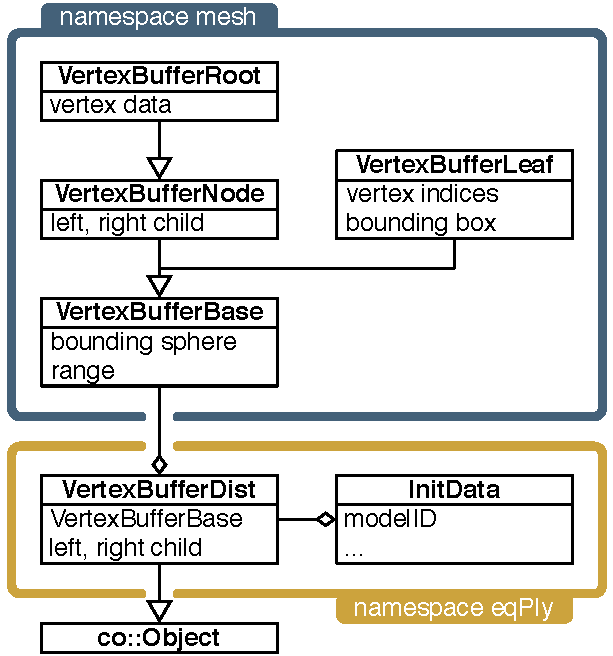
\includegraphics[width=.382\textwidth]{images/modelDist.pdf}
  {\caption{\small\label{fModelDist}Scene Data in eqPly}}
\end{wrapfigure}
The identifer of the root object of this distributed hierarchy is passed
as part of the \textsf{InitData}, and used during remote node
initialization to map the model. \fig{fModelDist} shows the UML
hierarchy of the model and distribution classes.

Each \textsf{VertexBufferDist} object has one node of the model's data
tree. It is serializing the data for this node. Furthermore, it mirrors
the kD-tree by having a \textsf{VertexBufferDist} child for each child
of its corresponding tree node. During serialization, the identifier of
these children is sent to the remote nodes, which reconstruct the mirror
distribution hierarchy and model data tree based on this data.

The serialization function \textsf{getInstanceData} sends all the data
needed to reconstruct the model tree: the object identifiers of its
children, vertex data for the tree root and vertex indices for the leaf
nodes, as well as the bounding sphere and database range of each
node. The deserialization function \textsf{applyInstanceData} retrieves
the data in multiple steps, and constructs the model tree on the fly
based on this information. It is omitted here for brevity:


{\footnotesize\begin{lstlisting}
void VertexBufferDist::getInstanceData( eq::net::DataOStream& os )
{
    EQASSERT( _node );
    os << _isRoot;

    if( _left && _right )
    {
        os << _left->getID() << _right->getID();

        if( _isRoot )
        {
            EQASSERT( _root );
            const mesh::VertexBufferData& data = _root->_data;
            
            os << data.vertices << data.colors << data.normals << data.indices;
        }
    }
    else
    {
        os << EQ_ID_INVALID << EQ_ID_INVALID;

        EQASSERT( dynamic_cast< const mesh::VertexBufferLeaf* >( _node ));
        const mesh::VertexBufferLeaf* leaf = 
            static_cast< const mesh::VertexBufferLeaf* >( _node );

        os << leaf->_vertexStart << leaf->_vertexLength << leaf->_indexStart
           << leaf->_indexLength;
    }

    os << _node->_boundingSphere << _node->_range;
}
\end{lstlisting}}%>>

\begin{wrapfigure}{r}{.618\textwidth}
  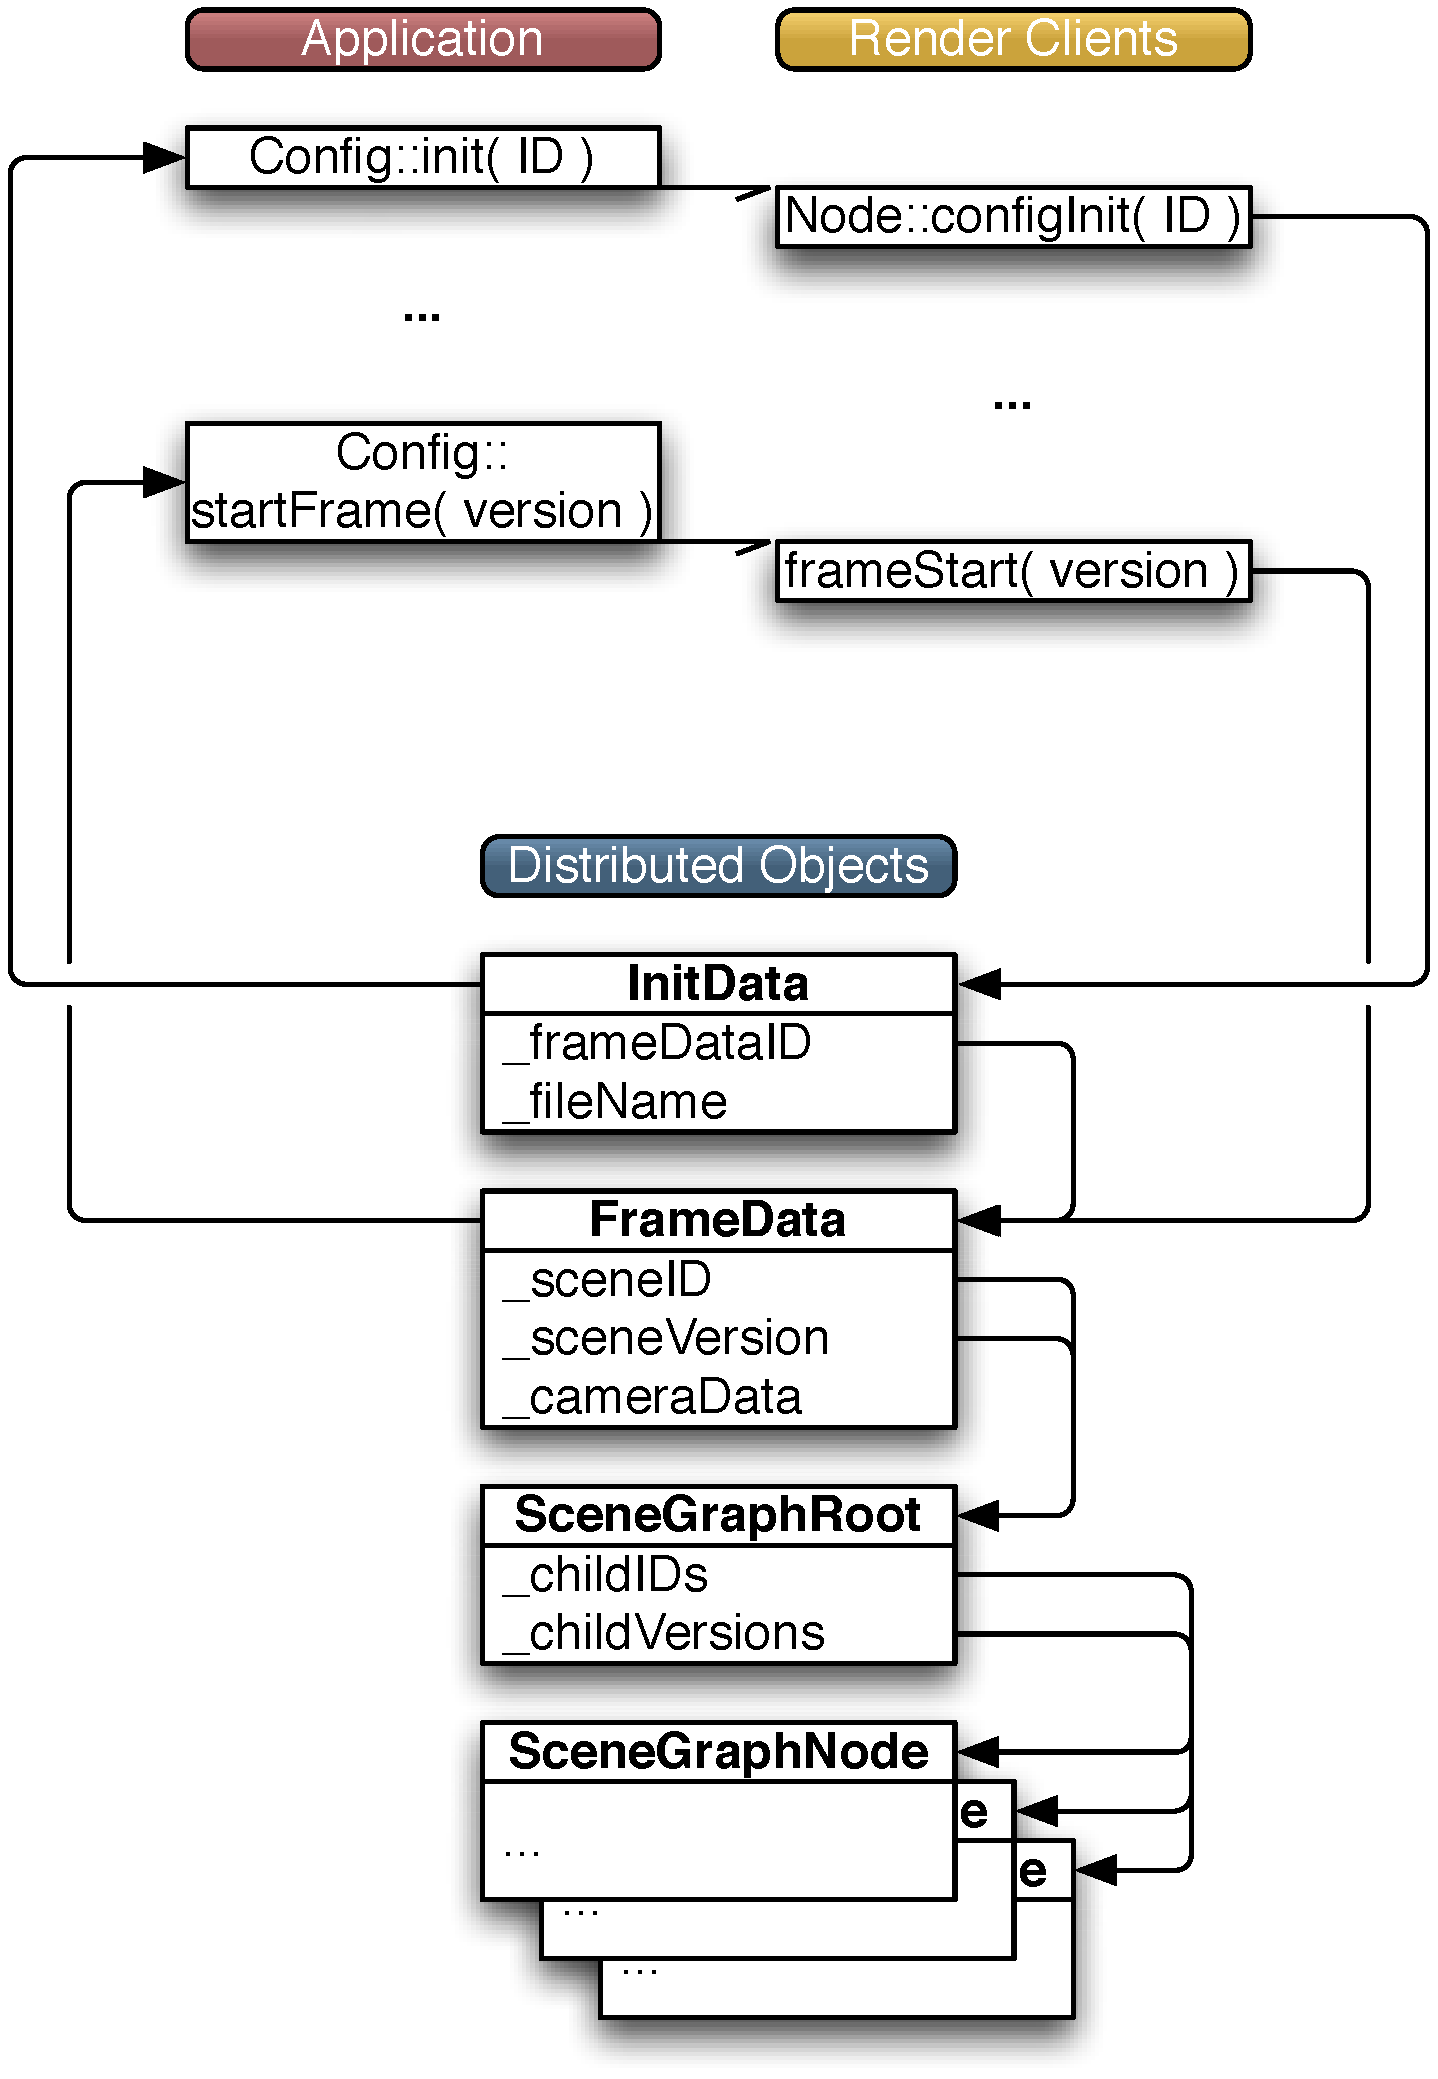
\includegraphics[width=.618\textwidth]{images/objects.pdf}
  {\caption{\small\label{fObjects}Scene Graph Distribution}}
\end{wrapfigure}
Applications distributing a dynamic scene graph use the frame data
instead of the init data as the entry point to their scene graph data
structure. \fig{fObjects} shows one possible implementation, where the
identifier and version of the scene graph root are transported using the
frame data. The scene graph root then serializes and de-serializes his
immediate children by transferring their identifier and current version,
similar to the static distribution done by \textsf{eqPly}.

The objects are still created by the application, and then registered or
mapped with the session in order to distribute them. When mapping
objects in a hierarchical data structure, their type often has to be
known in order to create them. Equalizer does not currently provide
object typing, this has to be done by the application, either implicitly
in the current implementation context, or by transferring a type
identifier. In \textsf{eqPly}, object typing is implicit since it is
well-defined which object is mapped in which context.


\subsection{Config}

The configuration is driving the application's rendering, that is, it is
responsible for updating the data based on received events, requesting
new frames to be rendered and to provide the render clients with the
necessary data.

\subsubsection{Initialization and Exit}

The config initialization happens in parallel, that is, all config
initialization tasks are transmitted by the server at once and their
completion is synchronized afterwards. 

The tasks are executed by the node and pipe threads in parallel. The
parent's initialization methods are always executed before any child
initialization method. This parallelization is necessary to allow a
speedy startup of the configuration on large-scale graphics clusters. On
the other hand, it means that initialization functions are called even
if the parent's initialization has failed.

The \textsf{eqPly::Config} class holds the master versions of the
initialization and frame data. Both objects are registered with the
\textsf{eq::Config}, which is the \textsf{eq::net::Session} used for
rendering. Equalizer takes care of the session setup and exit in
\textsf{Client::choose\-Config} and \textsf{Client::releaseConfig},
respectively.

The frame data is registered before the initialization data, since its
identifier is transmitted using the \textsf{InitData}. The identifier of
the initialization data is transmitted to the render client nodes using
the \textsf{initID} parameter of \textsf{eq::Config::init}.

Equalizer will pass this identifier to all \textsf{configInit} calls of
the respective objects:

{\footnotesize\begin{lstlisting}
bool Config::init()
{
    // init distributed objects
    _frameData.data.color = _initData.useColor();
    registerObject( &_frameData );
    _initData.setFrameDataID( _frameData.getID( ));

    registerObject( &_initData );

    // init config
    _running = eq::Config::init( _initData.getID( ));
    if( !_running )
        return false;
\end{lstlisting}}

\begin{wrapfigure}{r}{.618\textwidth}
  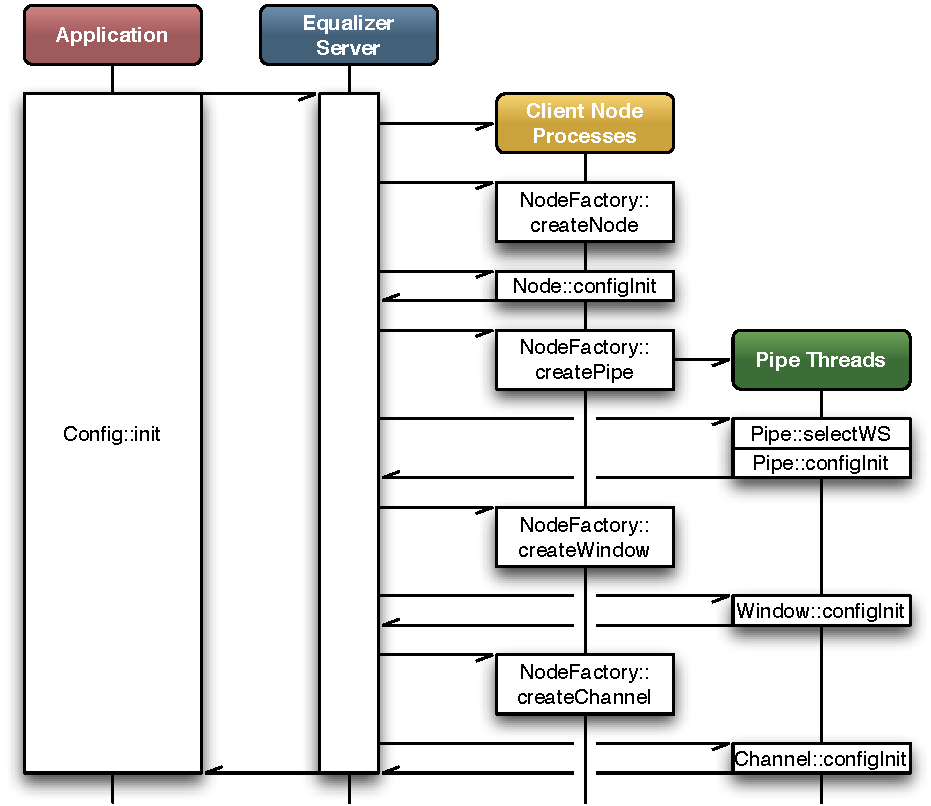
\includegraphics[width=.618\textwidth]{images/configInit.pdf}
  {\caption{\small\label{fConfigInit}Config Initialization Sequence}}
\end{wrapfigure}
If the configuration was initialized correctly, the configuration tries
to set up a tracking device for head tracking. Equalizer does not
provide extensive support for tracking devices, as this is an orthogonal
problem to parallel rendering. Tracking device support has already been
solved by a number of implementations\footnote{VRCO Trackd VRPN, etc.},
which can easily be integrated with Equalizer. The example code in
\textsf{eqPly} provides a reference implementation for the integration
of such a tracking library. \sref{sTracking} provides more background on
head tracking.

{\footnotesize\begin{lstlisting}
    // init tracker
    if( !_initData.getTrackerPort().empty( ))
    {
        if( !_tracker.init( _initData.getTrackerPort() ))
            EQWARN << "Failed to initialise tracker" << endl;
        else
        {
            // Set up position of tracking system in world space
            // Note: this depends on the physical installation.
            vmml::Matrix4f m( vmml::Matrix4f::IDENTITY );
            m.scale( 1.f, 1.f, -1.f );
            //m.x = .5;
            _tracker.setWorldToEmitter( m );

            m = vmml::Matrix4f::IDENTITY;
            m.rotateZ( -M_PI_2 );
            _tracker.setSensorToObject( m );
            EQLOG( eq::LOG_CUSTOM ) << "Tracker initialised" << endl;
        }
    }

    return true;
}
\end{lstlisting}}%>>

The exit function of the configuration stops the render clients by calling
\textsf{eq::Con\-fig::exit}, and then de-registers the initialization and
frame data objects with the session:

{\footnotesize\begin{lstlisting}
bool Config::exit()
{
    _running = false;
    const bool ret = eq::Config::exit();

    _initData.setFrameDataID( EQ_ID_INVALID );
    deregisterObject( &_initData );
    deregisterObject( &_frameData );

    return ret;
}
\end{lstlisting}}

\subsubsection{Frame Control}

The rendering frames are issued by the application. The
\textsf{eqPly::Config} only overrides \textsf{startFrame} in order to
update its data before forwarding the start frame request to the
\textsf{eq::Config}.

If a tracker is used, the current head position and orientation is
retrieved and passed to Equalizer, which uses the head matrix together
with the wall or projection description to compute the view
frustra\footnote{see
  \link{http://www.equalizergraphics.com/documents/design/immersive.html}}.

The camera position is updated and the frame data is commited, which
generates a new version of this object. This version is passed to the
rendering callbacks and will be used by the rendering threads to
synchronize the frame data to the state belonging to the current frame:

{\footnotesize\begin{lstlisting}
uint32_t Config::startFrame()
{
    // update head position
    if( _tracker.isRunning() )
    {
        _tracker.update();
        const vmml::Matrix4f& headMatrix = _tracker.getMatrix();
        setHeadMatrix( headMatrix );
    }

    // update database
    _frameData.data.rotation.preRotateX( -0.001f * _spinX );
    _frameData.data.rotation.preRotateY( -0.001f * _spinY );
    const uint32_t version = _frameData.commit();

    return eq::Config::startFrame( version );
}
\end{lstlisting}}


\subsubsection{Event Handling}

Events are sent by the render clients to the application using
\textsf{eq::Config::sendEvent}. At the end of the frame,
\textsf{Config::finishFrame} calls \textsf{Config::handleEvents} to do
the event handling. The default implementation processes all pending
events by calling \textsf{Config::handleEvent} for each of them.

For event-driven execution, the application can override
\textsf{Config::handleEvents} to blockingly receive events using
\textsf{Config::nextEvent} until a new frame has to be rendered.

The \textsf{eqPly} example continuously renders new frames. It
implements \textsf{Config::hand\-le\-Event} to provide the various reactions
to user input, most importantly camera updates based on mouse
events. The camera position has to be handled correctly with respect to
latency, and is therefore saved in the frame data:

{\footnotesize\begin{lstlisting}
bool Config::handleEvent( const eq::ConfigEvent* event )
{
    switch( event->type )
    {
        [...]
        case eq::ConfigEvent::POINTER_MOTION:
            if( event->pointerMotion.buttons == eq::PTR_BUTTON_NONE )
                return true;

            if( event->pointerMotion.buttons == eq::PTR_BUTTON1 )
            {
                _spinX = 0;
                _spinY = 0;

                _frameData.data.rotation.preRotateX( 
                    -0.005f * event->pointerMotion.dx );
                _frameData.data.rotation.preRotateY(
                    -0.005f * event->pointerMotion.dy );
            }
            else if( event->pointerMotion.buttons == eq::PTR_BUTTON2 ||
                     event->pointerMotion.buttons == ( eq::PTR_BUTTON1 |
                                                       eq::PTR_BUTTON3 ))
            {
                _frameData.data.translation.z +=
                    .005f * event->pointerMotion.dy;
            }
            else if( event->pointerMotion.buttons == eq::PTR_BUTTON3 )
            {
                _frameData.data.translation.x += 
                    .0005f * event->pointerMotion.dx;
                _frameData.data.translation.y -= 
                    .0005f * event->pointerMotion.dy;
            }
            return true;

        default:
            break;
    }
    return eq::Config::handleEvent( event );
}
\end{lstlisting}}


\subsection{Node}

For each active render client, one \textsf{eq::Node} instance is
created on the appropriate machine. Nodes are only instantiated on their
render client processes, i.e., each process should only have one
instance of the \textsf{eq::Node} class. The application process might
also have a node class, which is handled in exactly the same way as the
render client nodes. The application and render clients might use a
different node factory, instantiating a different type of \textsf{eq::Node}.

During node initialization the static, per-config data is mapped to a
local instance using the identifier passed from
\textsf{Config::init}. No pipe, window or channel tasks methods are
executed before \textsf{Node::configInit} has returned.

{\footnotesize\begin{lstlisting}
bool Node::configInit( const uint32_t initID )
{
    if( !eq::Node::configInit( initID ))
        return false;

    Config*    config = static_cast< Config* >( getConfig( ));
    return config->mapData( initID );
}
\end{lstlisting}}

The actual mapping of the static data is done by the config. The config
first retrieves the distributed \textsf{InitData}. The object is
directly unmapped since it is static, and the data has be retrieved.

The init data contains, among other things, the identifier of the
root of the model's kD-tree. Using this identifier, the model is mapped
to the node, as explained in \sref{sSceneData}:

{\footnotesize\begin{lstlisting}
bool Config::mapData( const uint32_t initDataID )
{
    if( _initData.getID() == EQ_ID_INVALID )
    {
        const bool mapped = mapObject( &_initData, initDataID );
        EQASSERT( mapped );
        unmapObject( &_initData ); // data was retrieved, unmap immediately
    }
    else  // appNode, _initData is registered already
        EQASSERT( _initData.getID() == initDataID );

    const uint32_t modelID = _initData.getModelID();
    if( modelID == EQ_ID_INVALID ) // no model loaded by application
        return true;

    if( !_model )
        _model = ModelDist::mapModel( this, modelID );

    return (_model != 0);
}
\end{lstlisting}}

Since the model data is static, the mirror tree for data distribution
is only created temporarily to retrieve the data. This is done in a
static function of the \textsf{VertexBufferDist} class. One instance of
the distribution class is mapped to the model's identifier. During
application of the instance data, it will map its children recursively:


{\footnotesize\begin{lstlisting}
mesh::VertexBufferRoot* VertexBufferDist::mapModel(eq::net::Session* session,
                                                   const uint32_t modelID )
{
    VertexBufferDist modelDist( 0, 0 );

    if( !session->mapObject( &modelDist, modelID ))
    {
        EQWARN << "Mapping of model failed" << endl;
        return 0;
    }

    modelDist._unmapTree(); // No longer needed    

    return const_cast< mesh::VertexBufferRoot* >( modelDist._root );
}
\end{lstlisting}}%>>

The two remaining functions in the node relax the thread synchronization
between the node and pipe threads, since all dynamic data is
multi-buffered in \textsf{eqPly}. \sref{sThreads} provides a detailed
explanation of thread synchronization in Equalizer:

{\footnotesize\begin{lstlisting}
void Node::frameDrawFinish( const uint32_t frameID,
                            const uint32_t frameNumber )
{ /* nop, see frameStart */ }

void Node::frameStart( const uint32_t frameID, const uint32_t frameNumber )
{
    startFrame( frameNumber ); // unlock pipe threads
    
    // Don't wait for pipes to release frame locally, sync not needed since all
    // dynamic data is multi-buffered
    releaseFrameLocal( frameNumber );
}
\end{lstlisting}}


\subsection{Pipe}

All task methods for a pipe and its children are executed in a separate
thread. This approach optimizes usage of the GPU, since all
tasks are executed serially and therefore do not compete for resources
or cause OpenGL context switches. Later versions of Equalizer might
introduce threaded windows to allow the parallel and independent
execution of rendering tasks on a single pipe.

\subsubsection{Initialization and Exit}

Pipe threads are not explicitely synchronized with each other, that is,
pipes might be rendering different frames at any given time. Therefore
frame-specific data has to be allocated for each pipe thread, which in
the \textsf{eqPly} example is the frame data. The frame data is a member
variable of the \textsf{eqPly::Pipe}, and is mapped to the identifier
provided by the initialization data. The initialization in
\textsf{eq::Pipe} does the GPU-specific initialization, which is
window-system-dependent. On AGL the display ID is determined, and on glX
the display connection is opened.

{\footnotesize\begin{lstlisting}
bool Pipe::configInit( const uint32_t initID )
{
    const Config*     config    = static_cast<Config*>( getConfig( ));
    const InitData& initData    = config->getInitData();
    const uint32_t  frameDataID = initData.getFrameDataID();
    eq::Config*     config      = getConfig();

    const bool mapped = config->mapObject( &_frameData, frameDataID );
    EQASSERT( mapped );

    return eq::Pipe::configInit( initID );
}
\end{lstlisting}}

The config exit function is similar to the config initialization. The
frame data is unmapped and GPU-specific data is de-initialized by
\textsf{eq::Config::exit}:

{\footnotesize\begin{lstlisting}
bool Pipe::configExit()
{
    eq::Config* config = getConfig();
    config->unmapObject( &_frameData );

    return eq::Pipe::configExit();
}
\end{lstlisting}}

\subsubsection{Window System}

Equalizer supports multiple window system interfaces, at the moment
glX/X11, WGL and AGL/Carbon. Some operating systems, and therefore some
Equalizer versions, support multiple window systems
concurrently\footnote{see
  \link{http://www.equalizergraphics.com/compatibility.html}}.

Each pipe might use a different window system for rendering, which is
determined before \textsf{Pipe::configInit} by
\textsf{Pipe::selectWindowSystem}. The default implementation of
\textsf{selectWindowSystem} loops over all window systems and returns
the first supported window system, determined by using
\textsf{supportsWindowSystem}.

The \textsf{eqPly} examples allows selecting the window system using a
command line option. Therefore the implementation of
\textsf{selectWindowSystem} is overwritten and returns the specified
window system, if supported:

{\footnotesize\begin{lstlisting}
eq::WindowSystem Pipe::selectWindowSystem() const
{
    const Config*            config = static_cast<Config*>( getConfig( ));
    const InitData&        initData = config->getInitData();
    const eq::WindowSystem ws       = initData.getWindowSystem();

    if( ws == eq::WINDOW_SYSTEM_NONE )
        return eq::Pipe::selectWindowSystem();
    if( !supportsWindowSystem( ws ))
    {
        EQWARN << "Window system " << ws 
               << " not supported, using default window system" << endl;
        return eq::Pipe::selectWindowSystem();
    }

    return ws;
}
\end{lstlisting}}%>>

\subsubsection{\label{sCarbonThread}Carbon/AGL Thread Safety}

Parts of the Carbon API used for window and event handling in the AGL
window system are not thread safe. The application has to call
\textsf{eq::Global::enterCarbon} before any thread-unsafe Carbon call,
and \textsf{eq::Global::leaveCarbon} afterwards. These functions should
be used only during window initialization and exit, not during
rendering. For various reasons \textsf{enterCarbon} might block up to 50
milliseconds. Carbon calls in the window event handling routine
\textsf{Window::processEvent} are thread-safe, since the global carbon
lock is set in this method. Please contact the Equalizer developer
mailing list if you need to use Carbon calls on a per-frame basis.

\subsubsection{Frame Control}

All task methods for a given frame of the pipe, window and channel
entities belonging to the thread are executed in one block, starting
with \textsf{Pipe::frameStart} and finished by
\textsf{Pipe::finishFrame}. The frame start callback is therefore the
natural place to update all frame-specific data to the version belonging
to the frame. 

In \textsf{eqPly}, the version of the only frame-specific object
\textsf{FrameData} is passed as the per-frame id from
\textsf{Config::startFrame} to the frame task methods. The pipe uses
this version to update its instance of the frame data to the current
version, and then unlocks its child entities by calling
\textsf{startFrame}:

{\footnotesize\begin{lstlisting}
void Pipe::frameStart( const uint32_t frameID, const uint32_t frameNumber )
{
    // don't wait for node to start frame, local sync not needed
    // node->waitFrameStarted( frameNumber );
    _frameData.sync( frameID );
    startFrame( frameNumber );
}
\end{lstlisting}}


\subsection{\label{sEqplyWIndow}Window}

The Equalizer window abstracts an OpenGL drawable and a rendering
context. When using the default window initialization functions, all
windows of a pipe share the OpenGL context. This allows reuse of OpenGL
objects such as display lists and textures between all windows of one
pipe.

The window class is the natural place for the application to maintain
all data specific to the OpenGL context.

\subsubsection{Window System Interface}

The particulars of creating a window and OpenGL context depend on the
window system used. One can either use the implementation provided by
the operating system, e.g., AGL, WGL or glX, or some higher-level
toolkit, e.g., Qt.

\begin{wrapfigure}{r}{.618\textwidth}
  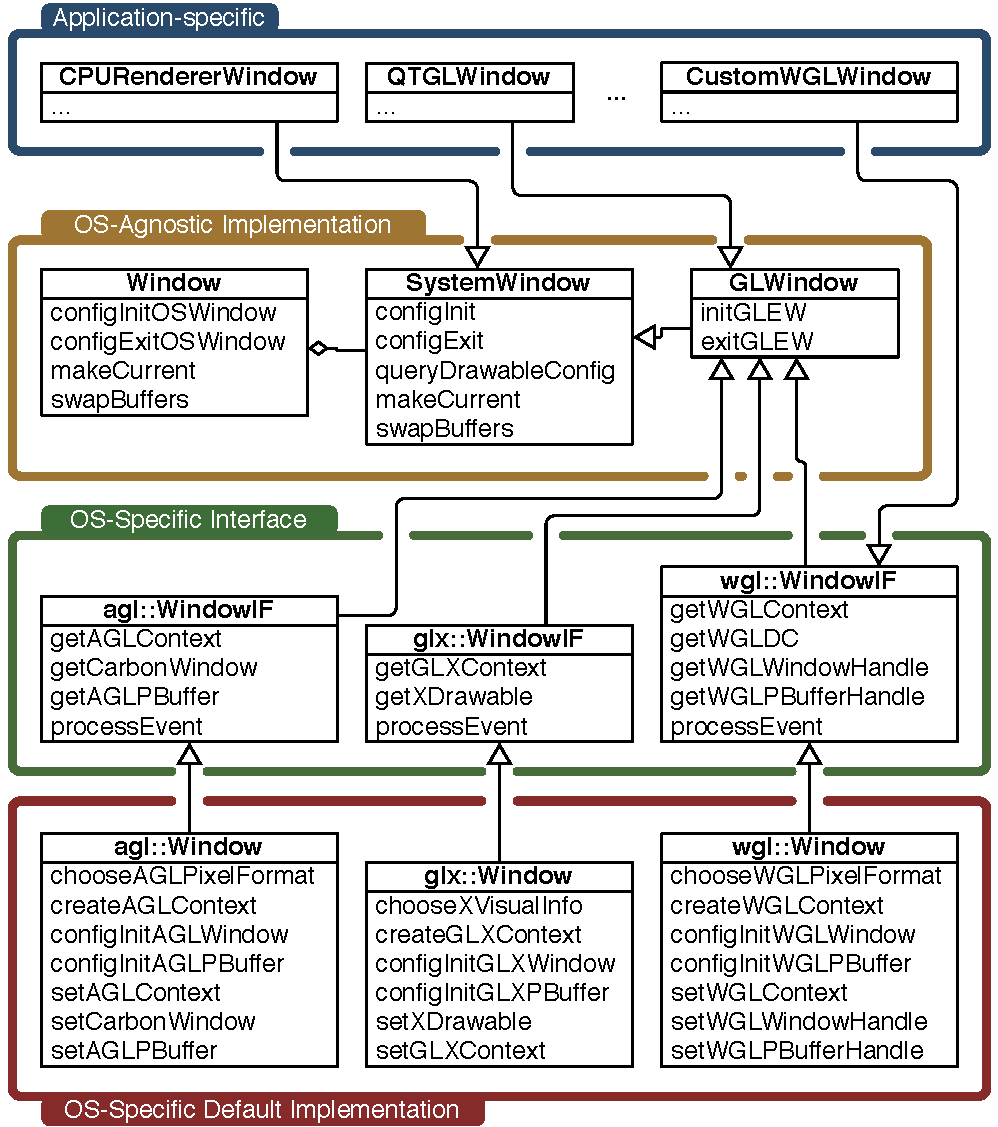
\includegraphics[width=.618\textwidth]{images/osWindow.pdf}
  {\caption{\small\label{fOSWindow}eq::OSWindow UML class hierarchy}}
\end{wrapfigure}
All window-system specific functionality is implemented by a
specialization of \textsf{eq::OS\-Window}. The \textsf{OSWindow} class
defines the minimal interface to be implemented for a new window
system. Each \textsf{Window} uses one \textsf{OSWindow} during
execution. This separation allows an easy implementation and adaption to
another window system or application.

Equalizer provides a generic interface and implementation for the three
most common window systems: AGL, WGL and glX. The interfaces define the
minimal functionality needed to reuse other window system specific
classes, for example the AGL, WGL and glX event handlers. The
implementation derived from these interfaces provides a sample
implementation which honors all configurable window attributes.

\subsubsection{Initialization and Exit}

The initialization sequence uses multiple, overrideable task
methods. The main task method \textsf{configInit} calls first
\textsf{configInitOSWindow}, which creates and initializes the
\textsf{OSWindow} for this window. The \textsf{OSWindow} initialization
code is implementation specific. If the \textsf{OSWindow} was
initialized successfully, \textsf{configInit} calls
\textsf{configInitGL}, which performs the generic OpenGL state
initialization. The default implementation sets up some typical OpenGL
state, e.g., it enables the depth test.

The \textsf{OSWindow} initialization takes into account various
attributes set in the configuration file. Attributes include the size of
the various frame buffer planes (color, alpha, depth, stencil) as well
as other framebuffer attributes, such as quad-buffered stereo,
doublebuffering, fullscreen mode and window decorations. Some of the
attributes, such as stereo, doublebuffer and stencil can be set to
\textsf{eq::AUTO}, in which case the Equalizer default implementation
will test for their availability and enable them if possible.

For the window-system specific initialization, \textsf{eqPly} uses the
default Equalizer implementation. The \textsf{eqPly} window
initialization only overrides the OpenGL-specific initialization
function \textsf{configInitGL} in order to initialize a state object and
an overlay logo. This function is only called if an OpenGL context was
created and made current:

{\footnotesize\begin{lstlisting}
bool Window::configInitGL( const uint32_t initID )
{
    if( !eq::Window::configInitGL( initID ))
        return false;

    glLightModeli( GL_LIGHT_MODEL_LOCAL_VIEWER, 1 );
    glEnable( GL_CULL_FACE ); // OPT - produces sparser images in DB mode
    glCullFace( GL_BACK );

    EQASSERT( !_state );
    _state = new VertexBufferState( getObjectManager( ));
    _loadLogo();

    const Config*   config   = static_cast< const Config* >( getConfig( ));
    const InitData& initData = config->getInitData();
    if( initData.useGLSL() )
        _loadShaders();

    return true;
}
\end{lstlisting}}%>>

The state object is used to handle the creation of OpenGL objects in a
multipipe, multi-threaded execution environment. It uses the object
manager of the \textsf{eq::Window}, which is described in detail in
\sref{sObjectManager}.

The logo texture is loaded from the file system and bound to a texture
ID used later by the channel for rendering. A code listing is ommitted,
since the code consists of standard OpenGL calls and is not
Equalizer-specific.

The window exit happens in the reverse order of the
initialization. First, \textsf{configExitGL} is called to de-initialize
OpenGL, followed by \textsf{configExitOSWindow} which de-initializes the
drawable and context and deletes the \textsf{OSWindow} allocated in
\textsf{configInitOSWindow}.

The window OpenGL exit function of \textsf{eqPly} de-allocates all
OpenGL objects. The object manager does not delete the object in its
destructor, since it does not know if an OpenGL context is still
current.

{\footnotesize\begin{lstlisting}
bool Window::configExitGL()
{
    if( _state )
        _state->deleteAll();

    delete _state;
    _state = 0;

    return eq::Window::configExitGL();
}
\end{lstlisting}}

\subsubsection{\label{sObjectManager}Object Manager}

The object manager is not strictly a part of the window. It
is mentioned here since the \textsf{eqPly} window uses an object manager.

The state object in \textsf{eqPly} gathers all rendering state, which
includes an object manager for OpenGL object allocation. 

The object manager (OM) is a utility class and can be used to manage
OpenGL objects across shared contexts. Typically one OM is used for each
set of shared contexts and spawns all contexts of a single
GPU\footnote{\link{http://www.equalizergraphics.com/documents/design/objectManager.html}}.

The OM is a template class. The template type is the key used to
identify objects. The same key is used by all contexts to get the
OpenGL name of an object.


Each \textsf{eq::Window} has an object manager with the key type
\textsf{const void*} for as long as it has an OpenGL context. The OM is
shared between all windows of a pipe, if the windows are created using
the default \textsf{configInit} functions. If the window is created by
the application, the OM is not shared since no assumption can be made
about OpenGL context sharing. Later version of Equalizer will introduce
an API to configure OpenGL context sharing, and therefore OM sharing, for
application-created windows.

\textsf{eqPly} uses the window's object manager in the rendering code to
obtain the OpenGL objects for a given data item. The address of the data
item to be rendered is used as the key. All objects managed by the OM
are reference counted. If an application releases the objects properly,
they are automatically de-allocated. It is also possible to manually
manage de-allocation of objects, which might be more convenient in some
cases.

Currently, support for display lists, VBO's, textures and shaders is
implemented. For each object, the following functions are available:

\begin{description}
\item[supportsObjects()] returns true if the usage for this particular
  type of objects is supported. For objects available in OpenGL 1.1 or
  earlier, this function is not implemented.
\item[getObject( key )] returns the object associated with the given
  key, or FAILED. Increases the reference count of existing objects.
\item[newObject( key )] allocates a new object for the given
  key. Returns FAILED if the object already exists or if the allocation
  failed. Sets the reference count of a newly created object to one.
\item[obtainObject( key )] convenience function which gets or obtains
  the object associated with the given key. Returns FAILED only if the
  object allocation failed.
\item[releaseObject( key \textbar\ name )] decreases the reference count and
  deletes the object if the reference count reaches zero.
\item[deleteObject( key \textbar\ name )] manually deletes the object. To be
  used if reference counting is not used.
\end{description}


\subsection{Channel}

The channel is the heart of the application in that it contains the
actual rendering code. The channel is used to perform the various rendering
operations for the compounds.

\subsubsection{Initialization and Exit}

During channel initialization, the near and far planes are set to
reasonable values to contain the whole model. During rendering, the near
and far planes are adjusted dynamically to the current model position:

{\footnotesize\begin{lstlisting}
bool Channel::configInit( const uint32_t initID )
{
    setNearFar( 0.1f, 10.0f );
    return true;
}
\end{lstlisting}}

\subsubsection{Rendering}

The central rendering routine is \textsf{Channel::frameDraw}. This
routine contains the application's OpenGL rendering code, which is being
rendered using the contextual information provided by Equalizer. As most
of the other task methods, \textsf{frameDraw} is called in parallel by
Equalizer on all pipe threads in the configuration. Therefore the
rendering must not write to shared data, which is the case for all major
scene graph implementations.

In \textsf{eqPly}, the OpenGL context is first set up using various
\textsf{apply} convenience methods from the base Equalizer channel
class. Each of the \textsf{apply} methods uses the corresponding
\textsf{get} method(s) and then calls the appropriate OpenGL
function(s). It is also possible to just query the values from Equalizer
using the \textsf{get} methods, and use them to set up the OpenGL state
appropriatly, for example by passing the parameters to the renderer used
by the application.

For example, the implementation for \textsf{eq::Channel::applyBuffer}
does set up the correct rendering buffer and color mask, which depends
on the current eye pass and possible anaglyphic stereo parameters:

{\footnotesize\begin{lstlisting}
void eq::Channel::applyBuffer()
{
    glReadBuffer( getReadBuffer( ));
    glDrawBuffer( getDrawBuffer( ));
    
    const ColorMask& colorMask = getDrawBufferMask();
    glColorMask( colorMask.red, colorMask.green, colorMask.blue, true );
}
\end{lstlisting}}

The contextual information has to be used in order to render the view as
expected by Equalizer. Failure to use certain information will result in
incorrect rendering for some or all configurations. The channel render
context consist of:

\begin{description}
\item[Buffer] The OpenGL read and draw buffer as well as color mask.
  These parameters are influenced by the current eye pass, eye
  separation and anaglyphic stereo settings.
\item[Viewport] The two-dimensional pixel viewport restricting the
  rendering area within the channel. For correct operations, both
  \textsf{glViewport} and \textsf{glScissor} have to be used. The pixel
  viewport is influenced by the destination channel's viewport
  definition and compound viewports set for sort-first/2D decompositions.
\item[Frustum] The same frustum parameters as defined by
  \textsf{glFrustum}. Typically the frustum used to set up the OpenGL
  projection matrix. The frustum is influenced by the destination
  channel's view definition, compound viewports, head matrix and the
  current eye pass.
\item[Head Transformation] A transformation matrix positioning the
  frustum. This is typically an identity matrix and is used for off-axis
  frustra in immersive rendering. It is normally used to set up the
  `view' part of the modelview matrix, before static light sources are
  defined.
\item[Range] A one-dimensional range with the interval [0..1]. This
  parameter is optional and should be used by the application to render
  only the appropriate subset of its data. It is influenced by the
  compound range attribute.
\end{description}

The \textsf{frameDraw} method in \textsf{eqPly} calls the
\textsf{frameDraw} method from the parent class, the Equalizer
channel. The default \textsf{frameDraw} method uses the apply
convenience functions to setup the OpenGL state for all render context
information, with the exception of the range which will be used later
during rendering:

{\footnotesize\begin{lstlisting}
void eq::Channel::frameDraw( const uint32_t frameID )
{
    applyBuffer();
    applyViewport();
    
    glMatrixMode( GL_PROJECTION );
    glLoadIdentity();
    applyFrustum();

    glMatrixMode( GL_MODELVIEW );
    glLoadIdentity();
    applyHeadTransform();
}

void Channel::frameDraw( const uint32_t frameID )
{
    // Setup OpenGL state
    eq::Channel::frameDraw( frameID );
\end{lstlisting}}

\begin{wrapfigure}{r}{.382\textwidth}
  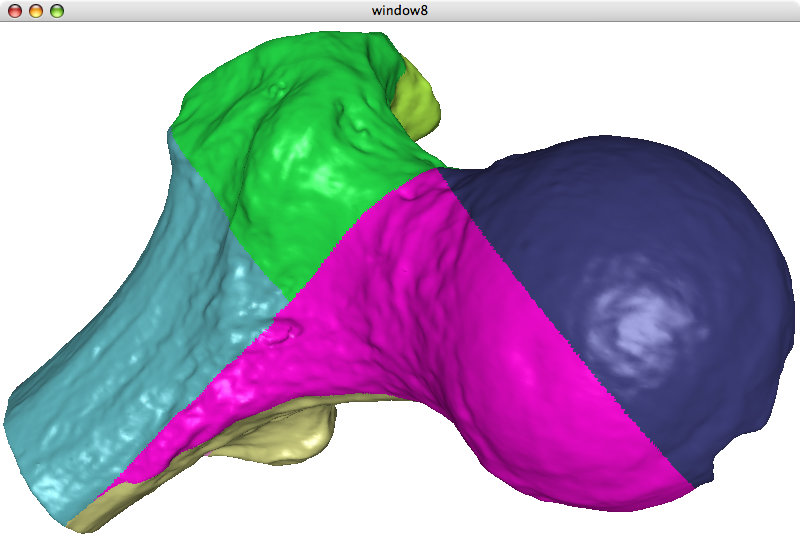
\includegraphics[width=.382\textwidth]{images/DB.png}
  {\caption{\small\label{fDB}Destination view of a DB compound}}
\end{wrapfigure}
After the basic view setup, a directional light is configured, and the
model is positioned using the camera parameters from the frame data. The
camera parameters are transported using the the frame data to ensure
that all channels render a given frame using the same position.

Furthermore, a white color is set in case the model does not contain
color information, or the color information is not used. In
sort-last rendering, \textsf{eqPly} uses a different color for each
channel to illustrate the database decomposition, as shown in
\fig{fDB}. The Equalizer channel provides a method to obtain a random,
but unique color for all channels in the configuration. This color is
determined by the server to ensure uniqueness across all channels of the
configuration:

{\footnotesize\begin{lstlisting}
    glLightfv( GL_LIGHT0, GL_POSITION, lightPosition );
    glLightfv( GL_LIGHT0, GL_AMBIENT,  lightAmbient  );
    glLightfv( GL_LIGHT0, GL_DIFFUSE,  lightDiffuse  );
    glLightfv( GL_LIGHT0, GL_SPECULAR, lightSpecular );

    glMaterialfv( GL_FRONT, GL_AMBIENT,   materialAmbient );
    glMaterialfv( GL_FRONT, GL_DIFFUSE,   materialDiffuse );
    glMaterialfv( GL_FRONT, GL_SPECULAR,  materialSpecular );
    glMateriali(  GL_FRONT, GL_SHININESS, materialShininess );

    const Pipe*      pipe      = static_cast<Pipe*>( getPipe( ));
    const FrameData& frameData = pipe->getFrameData();

    glTranslatef( frameData.data.translation.x,
                  frameData.data.translation.y,
                  frameData.data.translation.z );
    glMultMatrixf( frameData.data.rotation.ml );

    Config*          config = static_cast< Config* >( getConfig( ));
    const Model*     model  = config->getModel();
    const eq::Range& range  = getRange();

    if( !range.isFull( )) // Color DB-patches
    {
        const vmml::Vector3ub color = getUniqueColor();
        glColor3ub( color.r, color.g, color.b );
    }
    else if( !frameData.data.color || (model && !model->hasColors( )) )
    {
        glColor3f( 1.0f, 1.0f, 1.0f );
    }
    
\end{lstlisting}}

Finally the model, which has been loaded by the node, is rendered. If
the model was not loaded during node initialization, a quad is drawn in
its place:

{\footnotesize\begin{lstlisting}
    if( model )
    {
        _drawModel( model );
    }
    else
    {
        glColor3f( 1.f, 1.f, 0.f );
        glNormal3f( 0.f, -1.f, 0.f );
        glBegin( GL_TRIANGLE_STRIP );
        glVertex3f(  .25f, 0.f,  .25f );
        glVertex3f(  .25f, 0.f, -.25f );
        glVertex3f( -.25f, 0.f,  .25f );
        glVertex3f( -.25f, 0.f, -.25f );
        glEnd();
    }
}
\end{lstlisting}}

In order to draw the model, a helper class for view frustum culling is
set up using the view frustum from Equalizer and the camera position
from the frame data. The frustum helper computes the six frustum planes
from the projection and modelView matrices. During rendering, the
bounding spheres of the model are tested against these planes to
determine the visibility with the frustum.

Furthermore, the render state from the window and the database range
from the channel is obtained. The render state manages display list or
VBO allocation:

{\footnotesize\begin{lstlisting}
void Channel::_drawModel( const Model* model )
{
    Window*                  window    = static_cast<Window*>( getWindow() );
    mesh::VertexBufferState& state     = window->getState();

    const Pipe*              pipe      = static_cast<Pipe*>( getPipe( ));
    const FrameData&         frameData = pipe->getFrameData();

    const eq::Range&         range     = getRange();
    vmml::FrustumCullerf     culler;

    state.setColors( frameData.data.color && 
                     range.isFull() && 
                     model->hasColors() );
    _initFrustum( culler, model->getBoundingSphere( ));

    model->beginRendering( state );
        
\end{lstlisting}}

\begin{wrapfigure}{r}{.618\textwidth}
  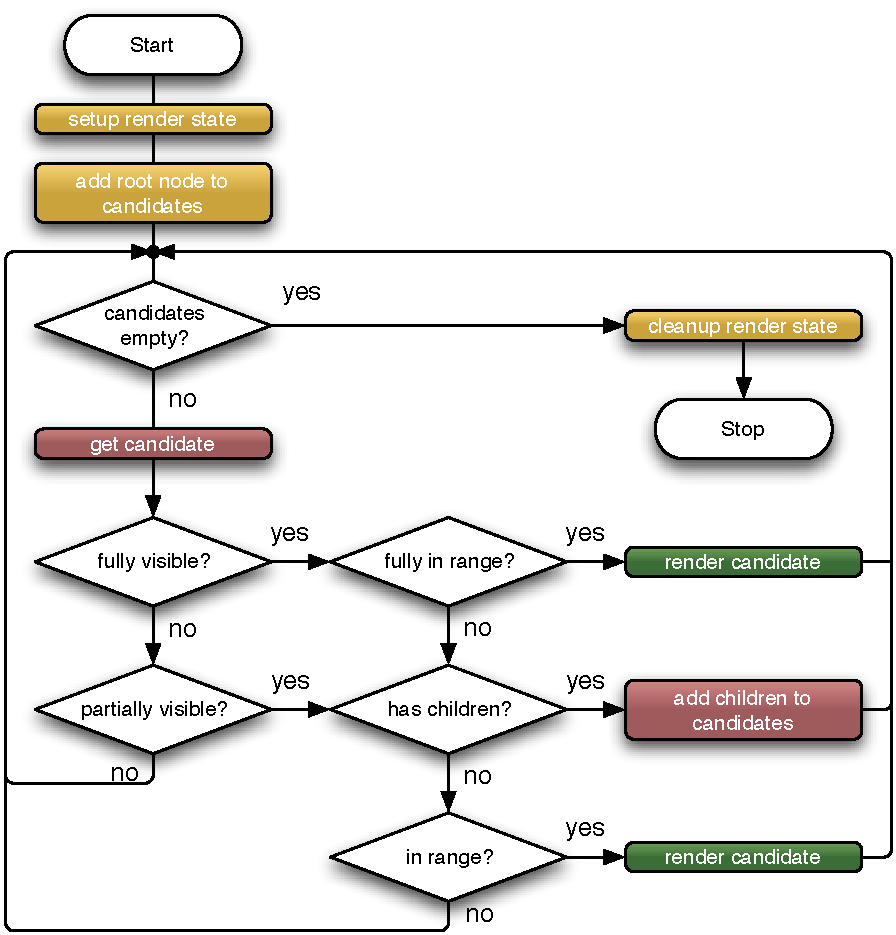
\includegraphics[width=.618\textwidth]{images/render.pdf}
  {\caption{\small\label{fRender}Main Render Loop}}
\end{wrapfigure}
The model data is spatially organized in an 3-dimensional
kD-tree\footnote{See also \link{http://en.wikipedia.org/wiki/Kd-tree}}
for efficient view frustum culling. When the model is loaded by
\textsf{Node::config\-Init}, it is preprocessed into the kD-tree and each
node of the tree gets a database range assigned. The root node
has the range [0, 1], its left child [0, 0.5] and its right child [0.5,
1], and so on for all nodes in the tree. The preprocessed model is saved
in a binary format for accelerating subsequent use.

The rendering loop maintains a list of candidates to render, which
initially contains the root node. Each candidate of this list is tested
for full visiblity against the frustum and range, and rendered if
visible. It is dropped if it is fully invisible or fully out of
range. If it is partially visible or partially in range, the children of
the node are added to the candidate list. \fig{fRender} shows a flow
chart of the rendering algorithm, which performs efficient view frustum
and range culling.

The actual rendering uses display lists or vertex buffer objects. These
OpenGL objects are allocated using the object manager. The rendering is
done by the leaf nodes, which are small enough to store the vertex
indices in a \textsf{short} value for optimal performance with VBO's.
The leaf nodes reuse the objects stored in the object manager, or create
and set up new objects if it was not yet set up. Since one object
manager is used per thread (pipe), this allows a thread-safe sharing of
the compiled display lists or VBO's across all windows of a pipe.

The main rendering loop in \textsf{eqPly} looks like this:

{\footnotesize\begin{lstlisting}
    model->beginRendering( state );
        
    // start with root node
    vector< const VertexBufferBase* > candidates;
    candidates.push_back( model );
        
    while( !candidates.empty() )
    {
        const VertexBufferBase* treeNode = candidates.back();
        candidates.pop_back();
            
        // completely out of range check
        if( treeNode->getRange()[0] >= range.end || 
            treeNode->getRange()[1] < range.start )
            continue;
            
        // bounding sphere view frustum culling
        switch( culler.testSphere( treeNode->getBoundingSphere() ) )
        {
            case vmml::VISIBILITY_FULL:
                // if fully visible and fully in range, render it
                if( treeNode->getRange()[0] >= range.start && 
                    treeNode->getRange()[1] < range.end )
                {
                    treeNode->render( state );
                    break;
                }
                // partial range, fall through to partial visibility
            case vmml::VISIBILITY_PARTIAL:
            {
                const VertexBufferBase* left = treeNode->getLeft();
                const VertexBufferBase* right = treeNode->getRight();
            
                if( !left && !right )
                {
                    if( treeNode->getRange()[0] >= range.start )
                        treeNode->render( state );
                    // else drop, to be drawn by 'previous' channel
                }
                else
                {
                    if( left )
                        candidates.push_back( left );
                    if( right )
                        candidates.push_back( right );
                }
                break;
            }
            case vmml::VISIBILITY_NONE:
                // do nothing
                break;
        }
    }
        
    model->endRendering( state );
}
\end{lstlisting}}


\section{Advanced Features}

This section discusses some additional important features not covered
by the previous \textsf{eqPly} section. Where possible, code examples
from the Equalizer distribution are used to illustrate one use case of
the feature.


\subsection{\label{sEventHandling}Event Handling}

Event handling requires a lot of flexibility. On one hand, the
implementation differs slightly for each operating and window system due
to conceptual differences in the specific implementation. On the
other hand, each application and widget set has its own model on how
events are to be handled. Therefore, event handling in Equalizer is
customizable at any stage of the processing, to the extreme of making it
possible to disable all event-related code in Equalizer. In this aspect,
Equalizer substantially differs from GLUT, which imposes an event model
and hides most of the event handling in \textsf{glutMainLoop}. More
information on event handling can be found on the Equalizer
website\footnote{see
  \link{http://www.equalizergraphics.com/documents/design/eventHandling.html}}.

The default implementation provides a convenient, easily accessible
event framework, while allowing all necessary customizations. It gathers
all events from all node processes in the main thread of the
application, so that the developer only has to implement
\textsf{Config::processEvent} to update its data based on the
pre-processed, generic keyboard and mouse events. It is very easy to use
and similar to an GLUT-based implementation.


\subsubsection{Threading}

In general, events are received and processed by the pipe thread a
window belongs to. An exception to this rule is AGL, where all events
are dispatched from the main node thread. WGL and GLX receive and
process the events from the pipe threads that created the
windows. Whenever the term \textbf{event thread} is used, it refers to
the thread receiving the event, i.e., the pipe thread for WGL and GLX,
and the main thread for AGL.

\subsubsection{Message Pump}

In order to dispatch events, Equalizer 'pumps' the native events. On
WGL and GLX, this happens on each thread with windows, whereas on
AGL it happens only on the main thread. By default, Equalizer
pumps these events automatically for the application in-between
executing task methods.

The methods \textsf{Client::useMessagePump} and
\textsf{Pipe::useMessagePump} can be overridden to return \textsf{false}
to disable this behaviour for their respective threads. On non-threaded
pipes, \textsf{Pipe::useMessagePump} is not called.

If the application disables message pumping in Equalizer, it has to make
sure the events are pumped externally, as it often done within external
widget sets such as Qt.

\subsubsection{Event Data Flow}

Events are received by an event handler. The event handler finds the
\textsf{eq::OSWindow} associated to the event. It then creates a generic
\textsf{Event}, which holds the event data in an independent
format. The original native event and this generic \textsf{Event}
form the \textsf{OSWindowEvent}, which is passed to the concrete
\textsf{OSWindow} for processing.

\begin{wrapfigure}{r}{.382\textwidth}
  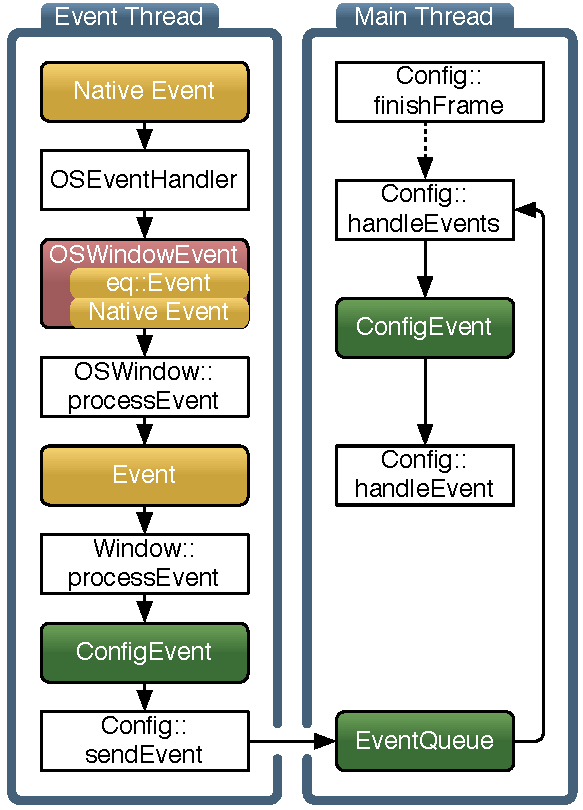
\includegraphics[width=.382\textwidth]{images/eventFilter.pdf}
  {\caption{\small\label{fEventProcessing}Event Processing}}
\end{wrapfigure}
The purpose of the \textsf{OSWindow} processing method,
\textsf{processEvent}, is to perform window-system specific event
processing. For example, \textsf{AGLWindow::processEvent} calls
\textsf{aglUpdateContext} whenever a resize event is received. For
further processing, the \textsf{Event} is passed on to
\textsf{Window::processEvent}. This \textsf{Event} no longer contains
the native event.

\textsf{Window::processEvent} is responsible for either handling
the event locally, or for translating it into a generic
\textsf{ConfigEvent}. The config events are send to the application
thread using \textsf{Config::sendEvent}. 

Events send using \textsf{Config::sendEvent} are queued in the
application thread. After a frame has been finished,
\textsf{Config::finishFrame} calls \textsf{Config::handleEvents}. The
default implementation of this method provides non-blocking event
processing, that is, it calls \textsf{Config::handleEvent} for each
queued event. By overriding \textsf{handleEvents}, event-driven
execution can easily be implemented.

If the event was processed, \textsf{processEvent} has to return
\textsf{true}. If \textsf{false} is returned to the event handler, the
event will be passed to the previously installed, window-system-specific
event handling function.

\fig{fEventProcessing} shows the overall data flow of an event.

\subsubsection{Default Implementation}

\begin{wrapfigure}{r}{.618\textwidth}
  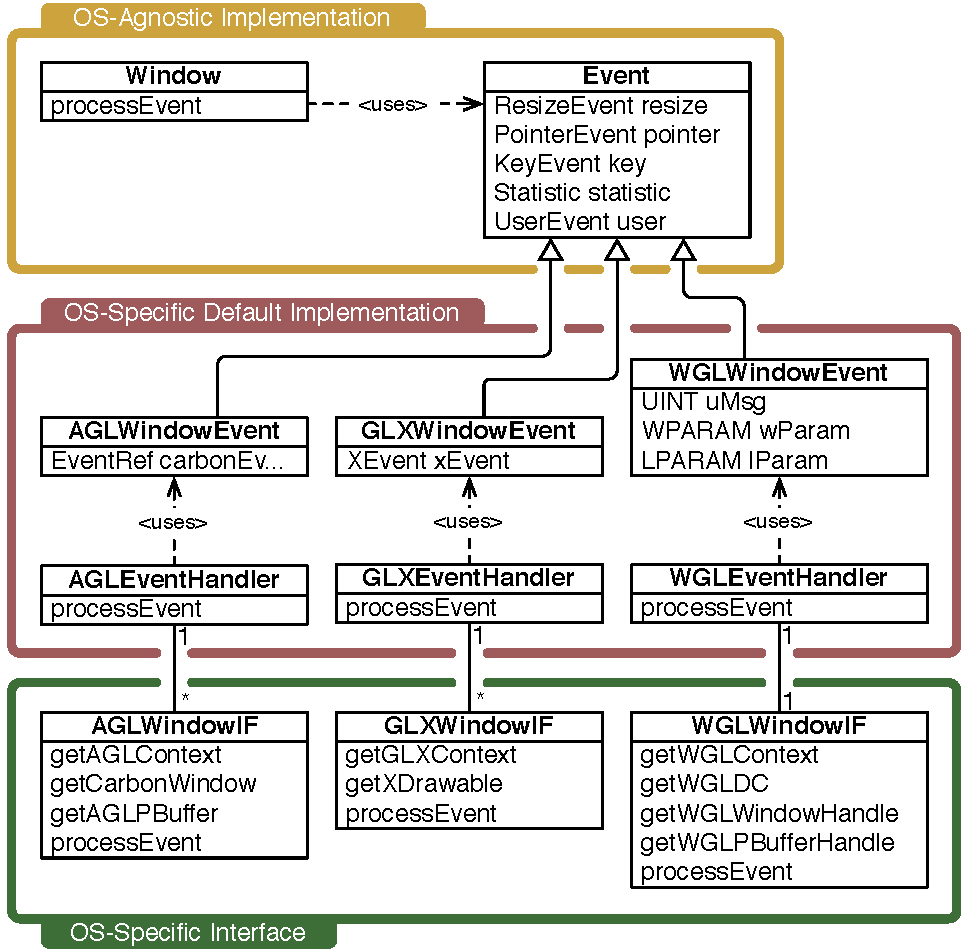
\includegraphics[width=.618\textwidth]{images/eventUML.pdf}
  {\caption{\small\label{fEventUML}UML Diagram for Event Handling Classes}}
\end{wrapfigure}
Currently, Equalizer provides an \textsf{AGLEvent\-Handler},
\textsf{GLXEventHandler} and \textsf{WGL\-Event\-Handler}, which handle
events for an \textsf{AGLWindowIF}, \textsf{GLXWindowIF} and
\textsf{WGLWindowIF}, respectively. \fig{fEventUML} illustrates the
class hierarchy for event processing.

The \textsf{OSWindow} implementation is responsible for setting up and
de-initializing event handling.

Carbon events issued for AGL windows are processed from the process main
thread. One \textsf{AGLEventHandler} is used. When a Carbon window is
set on an \textsf{AGLWindow}, the window is registered with the
\textsf{AGLEventHandler}. The event handler installs a Carbon event
handler for all important events. The event handler uses an
\textsf{AGLWindowEvent} to pass the Carbon \textsf{EventRef} to
\textsf{AGLWindowIF::processEvent}. During window exit, the installed
Carbon handler is removed when the window is deregistered with the
\textsf{AGLEventHandler}. No event handling is set up for PBuffers.

GLX uses one X11 Display connection for all windows on a GPU, which is
managed by the \textsf{eq::Pipe}. For each thread, one
\textsf{GLXEventHandler} is allocated. The pipe registers the display
connection with this per-thread event handler. Events for windows
created using this display connection are automatically received by the
event handler. No per-window event handling setup needs to be
done. PBuffers are handled in the same way as window drawables.

The glX event handler iterates over all windows of the registered pipe
to find the originating \textsf{GLXWindowIF}, which is then used to
process the event in a fashion similar to AGL. The
\textsf{GLXWindowEvent} passes the \textsf{XEvent} to
\textsf{GLXWindowIF::processEvent}.

Each \textsf{WGLWindow} allocates one \textsf{WGLEventHandler} when the
window handle is set. The WGLEventHandler passes the native event
parameters \textsf{uMsg}, \textsf{wParam} and \textsf{lParam} to
\textsf{WGLWindowIF::processEvent} as part of the
\textsf{WGLWindowEvent}. No event handling is set up for PBuffers.

Later Equalizer versions will introduce \textsf{Pipe::pro\-cess\-Event} and
\textsf{PipeEvent} to communicate pipe-specific events, e.g., monitor
resolution changes. It is also likely that an \textsf{OSPipe}
abstraction, similar to the \textsf{OSWindow}, will be created to
separate the window system specific code from the \textsf{eq::Pipe}.


\subsubsection{Custom Events in eqPixelBench}

The \textsf{eqPixelBench} example is a benchmark program to measure the
pixel transfer rates from and to the framebuffer of all channels within
a configuration. It uses custom config events to send the gathered data
to the application. It is much simpler than the \textsf{eqPly} example
since it does not provide any useful rendering or user interaction.

The rendering routine of \textsf{eqPixelBench} in
\textsf{Channel::frameDraw} loops through a number of pixel formats and
types. For each of them, it measures the time to readback and assemble a
full-channel image. The format, type, size and time is recorded in a
config event, which is sent to the application.

The \textsf{ConfigEvent} derives from the \textsf{eq::ConfigEvent}
structure and has the following definition:

{\footnotesize\begin{lstlisting}
struct ConfigEvent : public eq::ConfigEvent
{
public:
    enum Type
    {
        READBACK = eq::ConfigEvent::USER,
        ASSEMBLE
    };

    ConfigEvent()
        {
            size = sizeof( ConfigEvent );
        }

    // channel name is in user event data
    char           formatType[64];
    vmml::Vector2i area;
    float          msec;
};
\end{lstlisting}}

The \textsf{Config::sendEvent} method transmits an
\textsf{eq::ConfigEvent} or derived class to the application. The
ConfigEvent has to be a C-type structure, and its \textsf{size}
member has to be set to the full size of the event to be transmitted.
Each event has a type which is used to identify it by the config 
processing function.

User-defined types start at \textsf{eq::ConfigEvent::USER}, and the
member variable \textsf{ConfigEvent::user} can be used to store up to
\textsf{EQ\_USER\_EVENT\_SIZE}\footnote{currently 32 bytes} bytes. In
this space, the channel's name is stored. Additional variables are used
to transport the pixel format and type, the size and the time it took
for rendering.

On the application end, \textsf{Config::handleEvent} uses the
\textsf{ostream} operator for the derived config event to output these
events in a nicely formatted way:

{\footnotesize\begin{lstlisting}
std::ostream& operator << ( std::ostream& os, const ConfigEvent* event );
...
bool Config::handleEvent( const eq::ConfigEvent* event )
{
    switch( event->type )
    {
        case ConfigEvent::READBACK:
        case ConfigEvent::ASSEMBLE:
            cout << static_cast< const ConfigEvent* >( event ) << endl;
            return true;

        default:
            return eq::Config::handleEvent( event );
    }
}
\end{lstlisting}}%>>


\subsection{\label{sThreads}Multi-Threading and Synchronization}

Equalizer applications use multiple, asynchronous execution threads. The
default execution model is focused on making the porting of existing
applications as easy as possible, as described in \sref{sExecution}. The
default, per-node thread synchronization provided by Equalizer can
gradually be relaxed by advanced applications to gain better performance
through higher asynchronicity.

This section explains the multi-threading in Equalizer in detail and
gives advice on how to optimize applications for performance.

\subsubsection{Threads}

The application or node main thread is the primary thread of each
process and executes the \textsf{main} function. The application and
render clients initialize the local node for communications with other
nodes, including the server, using \textsf{Client::initLocal}.

\begin{wrapfigure}{r}{.618\textwidth}
  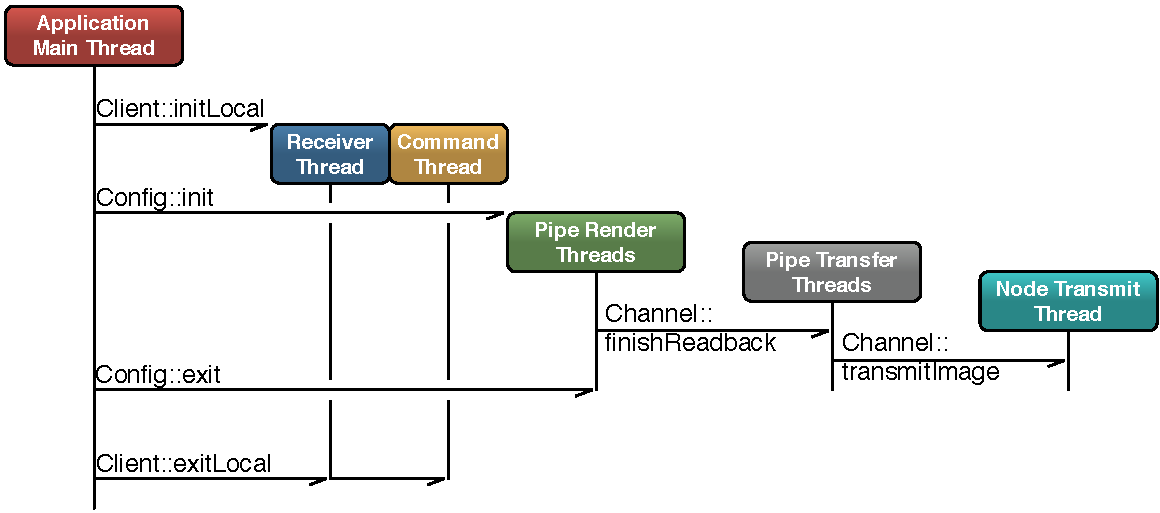
\includegraphics[width=.618\textwidth]{images/threads.pdf}
  {\caption{\small\label{fThreads}Threads within one node process}}
\end{wrapfigure}
During this initialization, Equalizer creates and manages two threads
for communication, the receiver thread and the command thread. Normally
no application code is executed from these two threads.

The receiver thread manages the network connections to other nodes and
receives data. It dispatches the received data either to the application
threads, or to the command thread.

The command thread processes Equalizer-related request from other nodes,
for example during \textsf{eq::net::Object} mapping. In some special cases
the command thread executes application code, for example when a remote
node maps a static or unbuffered object,
\textsf{Object::getInstanceData} is called from the command thread.

The receiver and command thread are terminated when the application
stops network communications using \textsf{Client::exitLocal}.

During config initialization, one pipe thread is created for each
pipe. The pipe threads execute all render task methods for this pipe,
and therefore executes the application's rendering code. The pipe
threads are terminated during \textsf{Config::exit}.

The rest of this section discusses the thread synchronization between
the main thread and the pipe threads.


\subsubsection{\label{sNodeFrame}Thread Synchronization Model}

The node main thread and the pipe threads are synchronized with each
other, so that all draw task methods of one rendered frame are executed
at the same time. This model allows to use the same database for
rendering, and safe modifications of this database are possible from the
node thread, since the pipe threads do not execute any rendering tasks
between frames.

Please note that the default thread synchronization synchronizes all
\textsf{Channel::frame\-Draw} operations on a \textbf{single} node with
the node's main thread. The per-node frame synchronization does not
break the asynchronous execution across nodes. Advanced applications can
remove the per-node frame synchronization.

The application has extended control over the task synchronization
during a frame. Upon \textsf{Config::startFrame}, Equalizer invokes the
\textsf{frameStart} task methods of the various entities. The entities
unlock all their children by calling \textsf{startFrame}, e.g.,
\textsf{Node::frameStart} has to call \textsf{Node::startFrame} in order
to unlock the pipe threads. Note that certain \textsf{startFrame} calls,
e.g., \textsf{Window::startFrame}, are currently empty since the
synchronization is implicit due to the sequential execution within the
thread.

\begin{wrapfigure}{r}{.618\textwidth}
  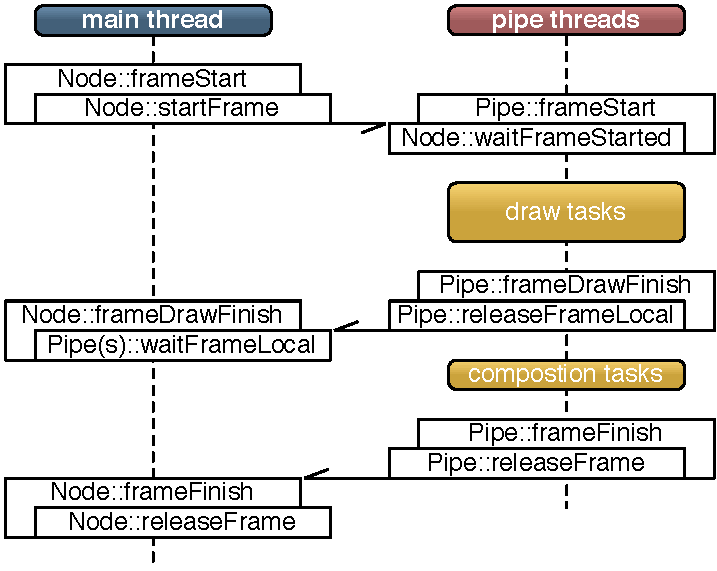
\includegraphics[width=.618\textwidth]{images/frameSync.pdf}
  {\caption{\small\label{fFrameSync}Per-Node Frame Synchronization}}
\end{wrapfigure}
Each entity uses \textsf{waitFrame\-Started} to block on the parent's
\textsf{startFrame}, e.g., \textsf{Pipe::\-frame\-Start} calls
\textsf{Node::wait\-Frame\-Started} to wait for the corresponding
\textsf{Node::start\-Fra\-me}. This explicit synchronization allows to
update non-critical data before synchronizing with
\textsf{waitFrameStarted}, or after unlocking using
\textsf{start\-Fra\-me}. \fig{fFrameSync} illustrates this
synchronization model.

At the end of the frame, two similar sets of synchronization methods are
used. The first set synchronizes the local execution, while the second
set synchronizes the global execution.

The local synchronization consists of \textsf{releaseFrameLocal} to
unlock the local frame, and of \textsf{waitFrameLocal} to wait for the
unlock. For the default synchronization model, Equalizer uses the task
method \textsf{frameDrawFinish} which is called on each resource
after the last \textsf{Channel::frameDraw} invocation for this
frame. Consequently, \textsf{Pipe::frameDrawFinish} calls
\textsf{Pipe::releaseFrame\-Lo\-cal} to signal that it is done drawing the
current frame, and \textsf{Node::frameDrawFinish} calls
\textsf{Pipe::waitFrameLocal} for each of its pipes to block the node
thread until the current frame has been drawn. 

\fig{fFrameSync} illustrates the local frame synchronization. By
removing the calls to \textsf{waitFrameLocal}, the node thread can
disable the synchronization with the pipe threads, which causes the node
operations to overlap with the rendering.

The second, global synchronization is used for the frame completion
during \textsf{Config::finishFrame}, which causes \textsf{frameFinish}
to be called on all entities, passing the oldest frame number, i.e., frame
\textsf{current-latency}. The \textsf{frameFinish} task methods have to
call \textsf{releaseFrame} to signal that the entitity is done with the
frame. The release causes the parent's \textsf{frameFinish} to be
invoked, which is synchronized internally. Once all
\textsf{Node::releaseFrame} have been called,
\textsf{Config::finishFrame} returns.

\begin{figure}[ht!]\center
  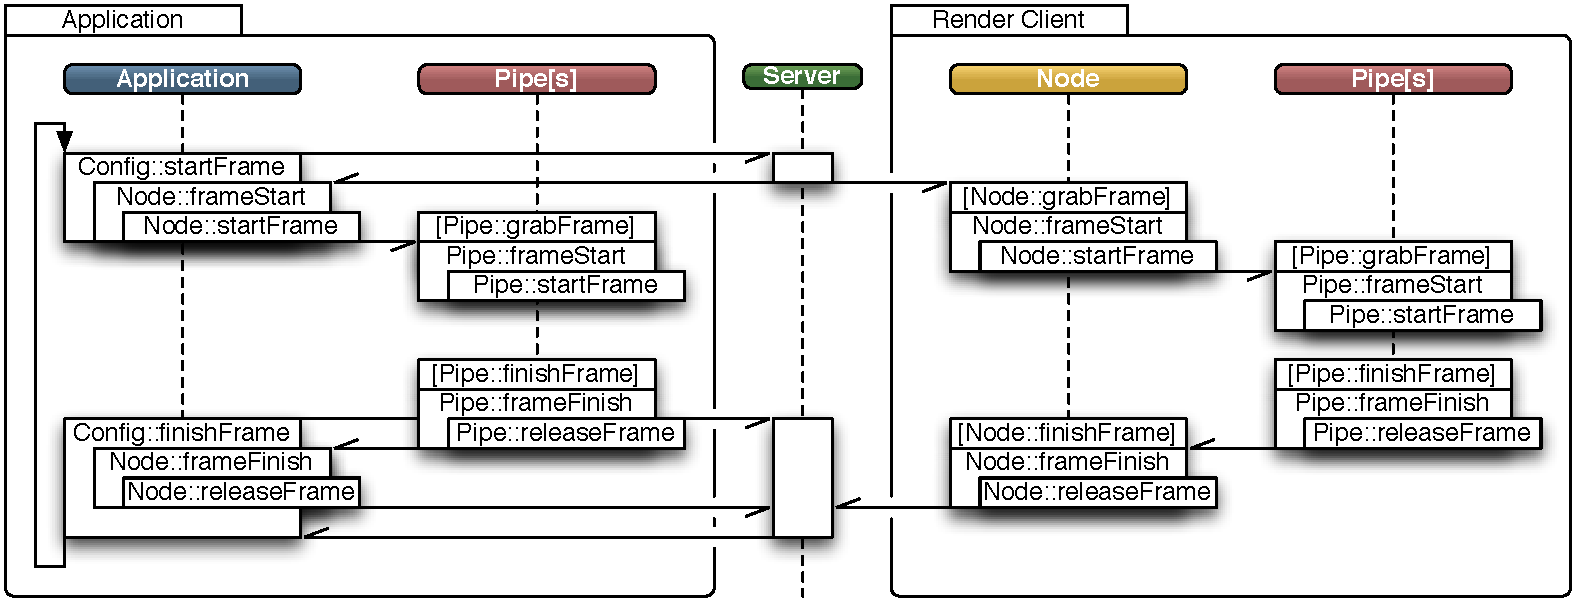
\includegraphics[width=\textwidth]{images/mainloop.pdf}
  {\caption{\small\label{fMainLoop}Synchronization of frame tasks}}
\end{figure}

\fig{fMainLoop} outlines the synchronization for the application, node
and pipe classes for an application node and one render client. Please
note that \textsf{Config::finishFrame} does block until the current
frame has been released locally and until the frame \textsf{current -
  latency} has been released by all nodes. The window and channel
synchronization are similar and omitted for simplicity.

It is absolutely vital for the execution that \textsf{Node::start\-Fra\-me}
and \textsf{Node::release\-Fra\-me} are called, respectively. The default
implementation of the node task methods does take care of that.

Since \textsf{eqPly} multi-buffers all dynamic data, it completely
removes frame synchronization by:

\begin{itemize}
\item releasing the local synchronization early in \textsf{Node::frameStart}
\item not waiting for the node to start the frame by not calling
  \textsf{Node::waitFrame\-Star\-ted} in \textsf{Pipe::frameStart}
\item not waiting for the pipe synchronization in
  \textsf{Node::frameDrawFinish} by not calling \textsf{Pipe::waitFrameLocal}
\end{itemize}



\subsection{OpenGL Extension Handling}

Equalizer uses GLEW\footnote{\link{http://glew.sourceforge.net}} for
OpenGL extension handling, particularly the GLEW MX implementation
providing multi-context support.

Each \textsf{eq::Window} has a \textsf{GLEWContext}. This context can be
obtained by using \textsf{glewGetContext} on the window or channel. GLEW
MX uses this function to dispatch the functions to the correct
context. Equalizer (re-)initializes the GLEW context whenever a new
OpenGL context is set on the window.

Extended OpenGL functions called from a window or channel instance can
be called directly. GLEW will call the object's \textsf{glewGetContext}
to obtain the correct context:

{\footnotesize\begin{lstlisting}
void eqPly::Channel::_drawModel( const Model* model )
{
    ...
    glUseProgram( program );
    ...
}
\end{lstlisting}}

Functions called from another place need to define a macro or function
\textsf{glewGetContext} that returns the pointer to the GLEWContext of
the appropriate window:

{\footnotesize\begin{lstlisting}
// state has GLEWContext* from window
#define glewGetContext state.glewGetContext

/*  Set up rendering of the leaf nodes.  */
void VertexBufferLeaf::setupRendering( VertexBufferState& state,
                                       GLuint* data ) const
{
    ...
    glBindBuffer( GL_ARRAY_BUFFER, data[VERTEX_OBJECT] );
    glBufferData( GL_ARRAY_BUFFER, _vertexLength * sizeof( Normal ),
                    &_globalData.normals[_vertexStart], GL_STATIC_DRAW );
    ...
}
\end{lstlisting}}


\subsection{Advanced Window Initialization}

This section explains window initialization in detail. It discusses in
detail the handling on the different window systems. The entry point for
the window initialization is the task method
\textsf{Window::configInit}. This task method first calls a
window-system-specific task method, and then
\textsf{Window::configInitGL} to do generic OpenGL state setup.

Since window initialization is notoriously error-prone and hard to
debug, the default Equalizer functions propagate the reason for errors
from the render clients back to the application. The \textsf{Pipe} and
\textsf{Window} classes have a \textsf{setErrorMessage} method, which is
used to set an error string. This string is passed to the
\textsf{Config} instance on the application node, where it can be
queried using \textsf{getErrorMessage}.

The window-system-specific initialization methods use overrideable
methods for all sub-tasks. This allows partial customization, without
the need of rewriting tedious window initialization code, e.g., the
OpenGL pixel format selection.

\subsubsection{\label{sDrawableConfig}Drawable Configuration}

OpenGL drawables have a multitude of buffer modes. A drawable might be
single-buffered, double-buffered or quad-buffered, have auxilary image
planes such as stencil, accumulation and depth buffer or multisampling.

The OpenGL drawable is configured using window attributes. These
attributes are used by the method choosing the pixel format (or visual
in X11 speak) to select the correct drawable configuration.

Window attributes can either be configured through the configuration
file (see \aref{aFileFormat}), or programmatically. In the configuration
file, modes are selected which are not application-specific, for example
stereo formats for active stereo displays. 

Applications which require certain drawable attributes can set the
corresponding window attribute hint during window initialization. The
Equalizer volume rendering example, \textsf{eVolve}, is such an
example. It does need alpha planes for rendering and compositing. The
window initialization of \textsf{eVolve} sets the attribute before
calling the default initialization method of Equalizer:

{\footnotesize\begin{lstlisting}
bool eVolve::Window::configInit( const uint32_t initID )
{
    // Enforce alpha channel, since we need one for rendering
    setIAttribute( IATTR_PLANES_ALPHA, 8 );

    return eq::Window::configInit( initID );
}
\end{lstlisting}}


\subsubsection{AGL Window Initialization}

AGL initialization happens in three steps: choosing a pixel format,
creating the context and creating a drawable. 

Most AGL and Carbon calls are not thread-safe. The Equalizer methods
calling these functions use \textsf{Global::enterCarbon} and
\textsf{Global::leaveCarbon} to protect the API calls. Please refer to
\sref{sCarbonThread} for more details.

The pixel format is chosen based on the window's attributes. Some
attributes set to auto, e.g., stereo, cause the method first to request
the feature and then to back off and retry if it is not available. The
returned pixel format has to be destroyed using
\textsf{Window::destroyAGLPixelFormat}. When no matching pixel format is
found, \textsf{chooseAGLPixelFormat} returns \textsf{0} and the AGL
window initialization returns with a failure.

The context creation also uses the global Carbon lock. Furthermore, it
sets up the swap buffer synchronization with the vertical retrace, if
enabled by the corresponding window attribute hint. Again the window
initialization fails if the context could not be created.

The drawable creation method \textsf{configInitAGLDrawable} calls either
\textsf{configInitAGLFullscreen}, \textsf{configInitAGLWindow} or \textsf{configInitAGLPBuffer}

The top-level AGL window initialization code therefore looks as follows:

{\footnotesize\begin{lstlisting}
bool Window::configInitAGL()
{
    AGLPixelFormat pixelFormat = chooseAGLPixelFormat();
    if( !pixelFormat )
        return false;

    AGLContext context = createAGLContext( pixelFormat );
    destroyAGLPixelFormat ( pixelFormat );
    setAGLContext( context );

    if( !context )
        return false;

    return configInitAGLDrawable();
}
\end{lstlisting}}


\subsubsection{GLX Window Initialization}

GLX initialization is very similar to AGL initialization. Again the
steps are: choose visual (pixel format), create OpenGL context and then
create drawable. The only difference is that the data returned by
\textsf{chooseXVisualInfo} has to be freed using \textsf{XFree}:

{\footnotesize\begin{lstlisting}
bool Window::configInitGLX()
{
    XVisualInfo* visualInfo = chooseXVisualInfo();
    if( !visualInfo )
        return false;

    GLXContext context = createGLXContext( visualInfo );
    setGLXContext( context );

    if( !context )
        return false;

    const bool success = configInitGLXDrawable( visualInfo );
    XFree( visualInfo );

    if( success && !_xDrawable )
    {
        setErrorMessage( "configInitGLXDrawable did set no X11 drawable" );
        return false;
    }

    return success;    
}
\end{lstlisting}}


\subsubsection{WGL Window Initialization}

The WGL initialization requires another order of operations compared to
AGL or GLX. The following functions are used to initialize a WGL window:

\begin{enumerate}
\item\textsf{getWGLPipeDC} is used to get an affinity device context,
  which might be needed for window creation. If a context is returned, a
  function pointer to delete the returned device context is set as
  well. This function might return 0, which is not an error.
\item\textsf{chooseWGLPixelFormat} chooses a pixel format based on the
  window attributes. If no device context is given, it uses the system
  device context. The chosen pixel format is set on the passed device
  context.
\item\textsf{configInitWGLDrawable} creates the drawable. The device
  context passed to \textsf{configInitWGLDrawable} is used to query the
  pixel format and is used as the device context for creating a
  PBuffer. If no device context is given, the display device context is
  used. On success, it sets the window handle. Setting a window handle
  also sets the window's device context.
\item\textsf{createWGLContext} creates an OpenGL rendering context using
  the given device context. If no device context is given, the window's
  device context is used. This function does not set the window's OpenGL
  context.
\end{enumerate}

The full \textsf{configInitWGL} task method, including error handling
and cleanup, looks as follows:

{\footnotesize\begin{lstlisting}
bool Window::configInitWGL()
{
    PFNEQDELETEDCPROC deleteDCProc = 0;
    HDC dc = getWGLPipeDC( deleteDCProc );
    EQASSERT( !dc || deleteDCProc );

    int pixelFormat = chooseWGLPixelFormat( dc );
    if( pixelFormat == 0 )
    {
        if( dc )
            deleteDCProc( dc );
        return false;
    }

    if( !configInitWGLDrawable( dc, pixelFormat ))
    {
        if( dc )
            deleteDCProc( dc );
        return false;
    }

    if( !_wglDC )
    {
        if( dc )
            deleteDCProc( dc );
        setErrorMessage( "configInitWGLDrawable did not set a WGL drawable" );
        return false;
    }

    HGLRC context = createWGLContext( dc );
    setWGLContext( context );

    if( !context )
    {
        if( dc )
            deleteDCProc( dc );
        return false;
    }

    if( dc )
        deleteDCProc( dc );
    return true;
}
\end{lstlisting}}


\subsection{\label{sTracking}Head Tracking}

The \textsf{eqPly} example contains rudimentary support for head
tracking, in order to show how head tracking can be integrated with
Equalizer. Support for a wide range of tracking devices is not within the
scope of Equalizer. Other open source and commercial implementations
cover this functionality sufficiently and can easily be integrated with
Equalizer.

\begin{figure}[h!t]
  \subfigure[]{\label{fMono}
    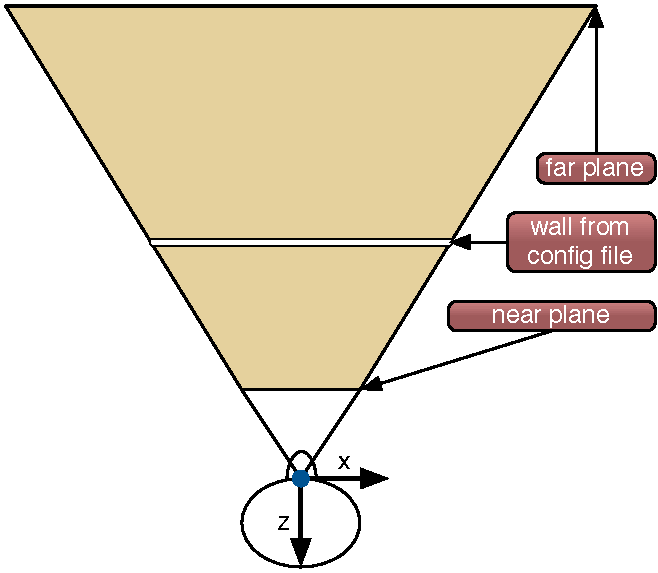
\includegraphics[height=3.5cm]{images/mono}}\hfil
  \subfigure[]{\label{fStereo}
    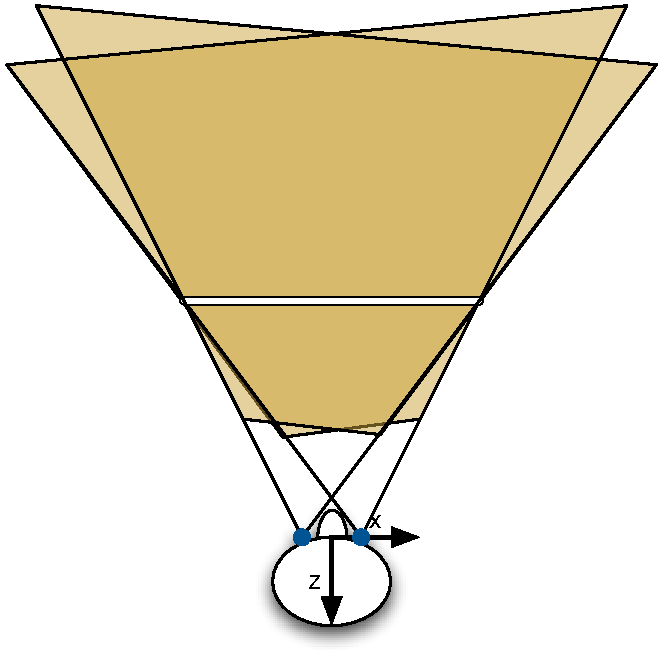
\includegraphics[height=3.5cm]{images/stereo}}\hfil
  \subfigure[]{\label{fTracked}
    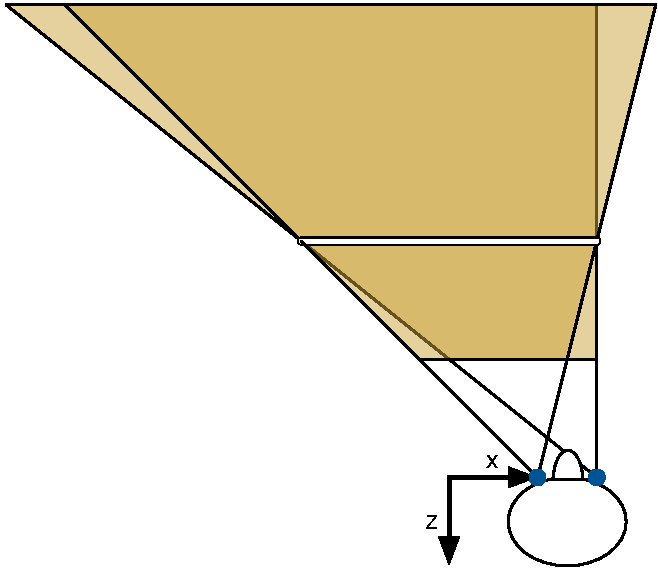
\includegraphics[height=3.5cm]{images/tracked}}%
  {\caption{\small\label{fImmersive}Monoscopic, Stereoscopic and Tracked
    frustra}}
\end{figure}

\fig{fMono} illustrates a monoscopic view frustum. The viewer is
positioned at the origin of the global coordinate system, and the
frustum is completely symmetric. This is the typical view frustum for
non-stereoscopic applications.

In stereo rendering, the scene is rendered twice, with the two frustra
'moved' by the distance between the eyes, as shown in \fig{fStereo}.

In immersive visualization, the observer is tracked in and the view
frustra are adapted to the viewer's position and orientation, as shown
in \fig{fTracked}. The transformation $origin \rightarrow viewer$ is set by
the application using \textsf{Config::setHeadMatrix}, which is used by
the server to compute the frustra. The resulting off-axis frustra are
positioned using the channel's head transformation, which can be
retrieved using \textsf{Channel::getHeadTransform}.


\subsection{\label{sCompositing}Image Compositing for Scalable Rendering}

Two task methods are responsible for collecting and compositing the
result image during scalable rendering. Scalable rendering is a use case
of parallel rendering, when multiple channels are contributing to a single
view. 

The source channels producing one or more \textsf{outputFrame}s use
\textsf{Channel::frame\-Read\-back} to read the pixel data from the frame
buffer. The channels receiving one or multiple \textsf{inputFrame}s use
\textsf{Channel::frameAssemb\-le} to assemble the pixel data into the
framebuffer. Equalizer takes care of the network transport of frame
buffer data between nodes.

Normally the programmer does not need to interfere with the image
compositing. Changes are sometimes required at a high level, for example
to order the input frames or to optimize the readback. The following
sections provide a detailed description of the image compositing API in
Equalizer.

\subsubsection{Parallel Direct Send Compositing}

In order to provide a motivation for the design of the image compositing
API, the direct send parallel compositing algorithm is introduced in this
section. Other parallel compositing algorithms, e.g. binary-swap, can
also be expressed through an Equalizer configuration file.

The main idea behind direct send is to parallelize the costly
recomposition for database (sort-last) decomposition. With each
additional source channel, the amount of pixel data to be composited
grows linearly. When using the simple approach of compositing all frames
on the destination channel, this channel quickly becomes the bottleneck
in the system. Direct send distributes this workload evenly across all
source channels, and thereby keeps the compositing work per channel
constant.

\begin{wrapfigure}{r}{.618\textwidth}
  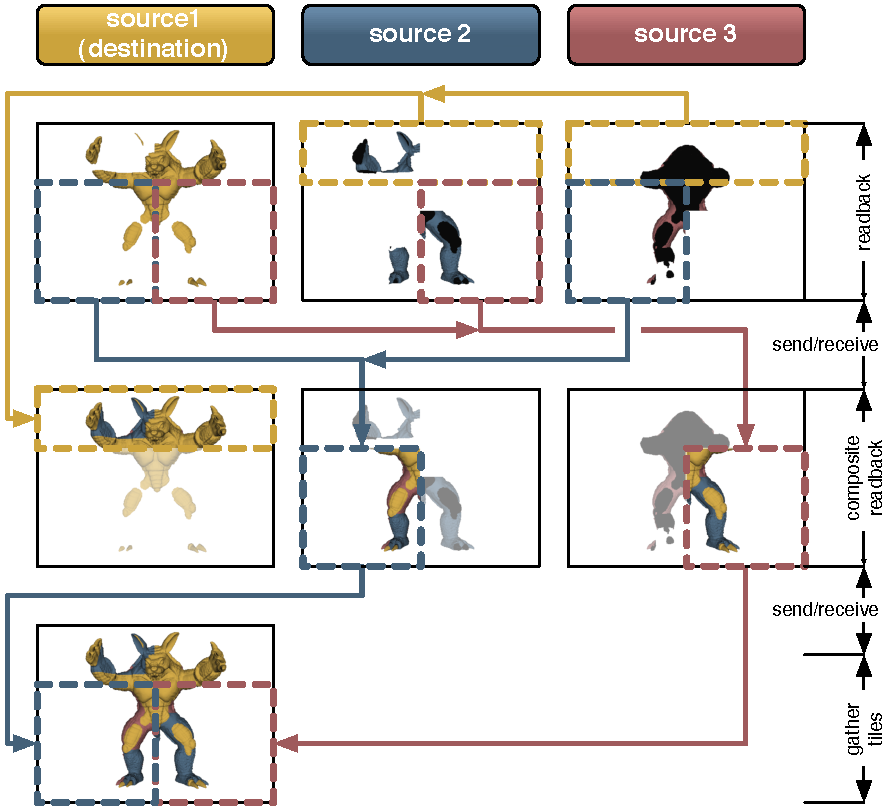
\includegraphics[width=.618\textwidth]{images/directSend.pdf}
  {\caption{\small\label{fDirectSend}Parallel Direct Send Compositing}}
\end{wrapfigure}
In direct send compositing, each rendering channel is also responsible
for the sort-last composition of one screen-space tile. He receives
the framebuffer pixels for his tile from all the other channels. The
size of one tile decreases linearly with the number of source channels,
which keeps the total amount of pixel data per channel constant.

After performing the sort-last compositing, the color information is
transferred to the destination channel, similarly to a 2D (sort-first)
compound. The amount of pixel data for this part of the compositing
pipeline also approaches a constant value, i.e., the full frame buffer.

\fig{fDirectSend} illustrates this algorithm for three channels. The
Equalizer website contains a
presentation\footnote{\link{http://www.equalizergraphics.com/documents/EGPGV07.pdf}}
explaining and comparing this algorithm with the binary-swap algorithm.

The following operations have to be possible in order to perform this
algorithm:
\begin{itemize}
\item Selection of color and/or depth frame buffer attachments
\item Restricting the read-back area to a part of the rendered area
\item Positioning the pixel data correctly on the receiving channels
\end{itemize}

Furthermore it should be possible for the application to implement a
read back of only the relevant region of interest, that is, the 2D area
of the framebuffer actually updated during rendering. This optimization
will be fully supported by later versions of Equalizer.

\subsubsection{Frame, Frame Data and Images}

An \textsf{eq::Frame} references an \textsf{eq::Fra\-me\-Data}. The
frame data is the object connecting output with input frames. Output and
input frames with the same name within the same compound tree will
reference the same frame data.

The frame data is a holder for images and additional information, such
as output frame attributes and pixel data availability.

An \textsf{eq::Image} holds a
two-dimensional snapshot of the framebuffer and can contain color and/or
depth information.

The frame synchronization through the frame data allows the input frame
to wait for the pixel data to become ready, which is signalled by the
output frame after readback.

Furthermore, the frame data transports the inherited range of the output
frame's compound. The range can be used to compute the assembly order of
multiple input frames, e.g., for sorted-blend compositing in volume
rendering applications.

\begin{wrapfigure}{r}{.618\textwidth}
  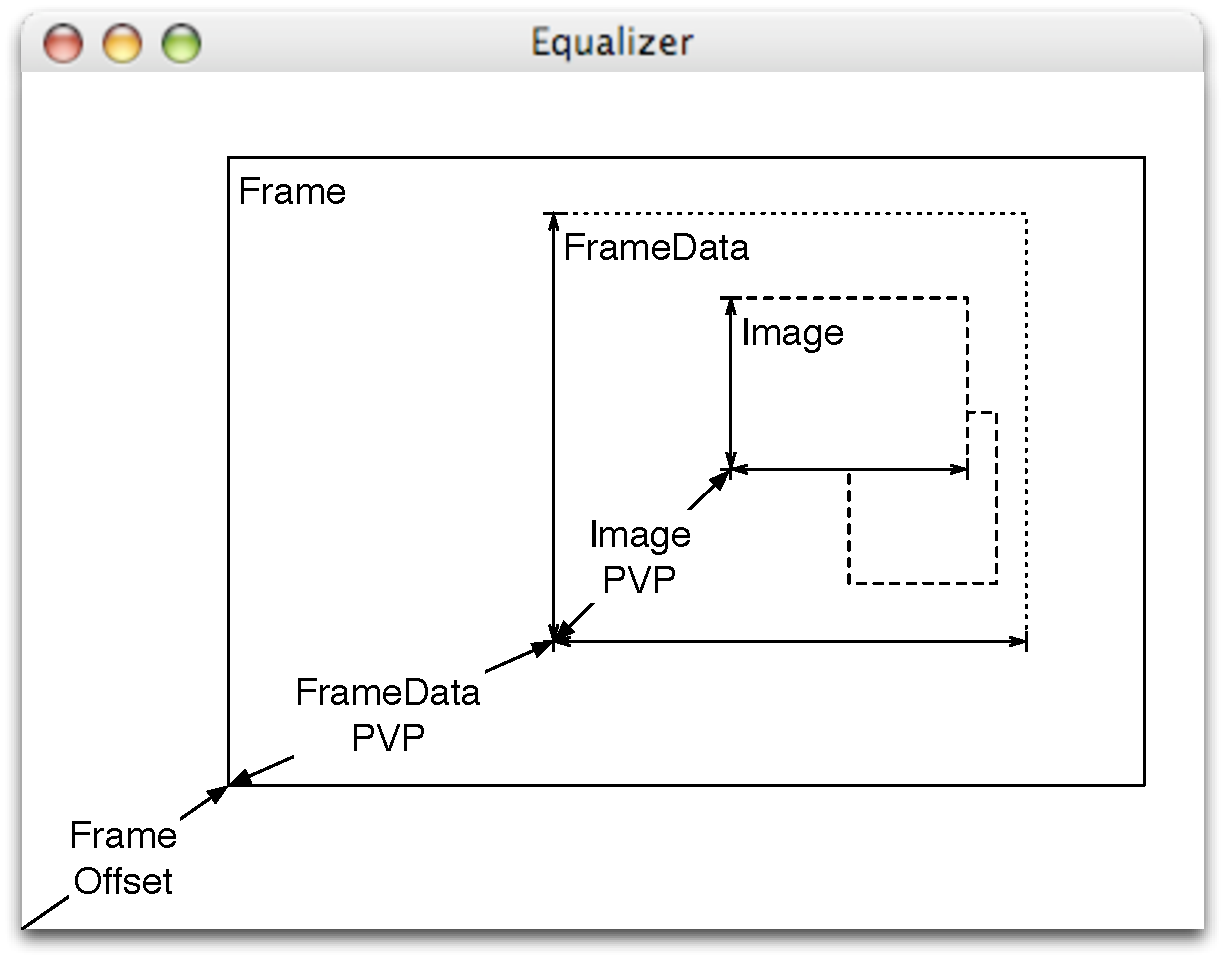
\includegraphics[width=.618\textwidth]{images/assembly.pdf}
  {\caption{\small\label{fAssembly}Hierarchy of assembly classes}}
\end{wrapfigure}
Readback and assemble operations on frames and images are designed to be
asynchronous. They have a start and finish method for both readback and
assemble to allow the initiation and synchronization of the operation.
Currently, only synchronous readback and assembly using
\textsf{glReadPixels} and \textsf{glDrawPixels} is implemented in the
respective start method of the image. Later versions of Equalizer will
implement asynchronous pixel transfers.

The offset of input and output frames characterizes the position of the
frame data with respect to the framebuffer, that is, the
\textbf{window's} lower-left corner. For output frames this is the
position of the channel with respect to the window.

For output frames, the frame data's pixel viewport is the area of the
frame buffer to read back. It will transport the offset from the source
to the destination channel, that is, the frame data pixel viewport for
input frames position the pixel data on the destination. This has the
effect that a partial framebuffer readback will end up in the same place
in the destination channels.

The image pixel viewport signifies the region of interest that will be read
back. The default readback operation reads back one image using the full
pixel viewport of the frame data.

\fig{fAssembly} illustrates the relationship between frames, frame data
and images.

\subsubsection{Custom Assembly in eVolve}

The \textsf{eVolve} example is a scalable volume renderer. It uses 3D
texture-based volume rendering, where the 3D texture is intersected by
view-aligned slices. The slices are rendered back-to-front and blended
together to produce the final image, as shown in
\fig{fSlices}\footnote{Volume Data Set courtesy of: SFB-382 of the German
  Research Council (DFG)}.

\begin{wrapfigure}{r}{.382\textwidth}
  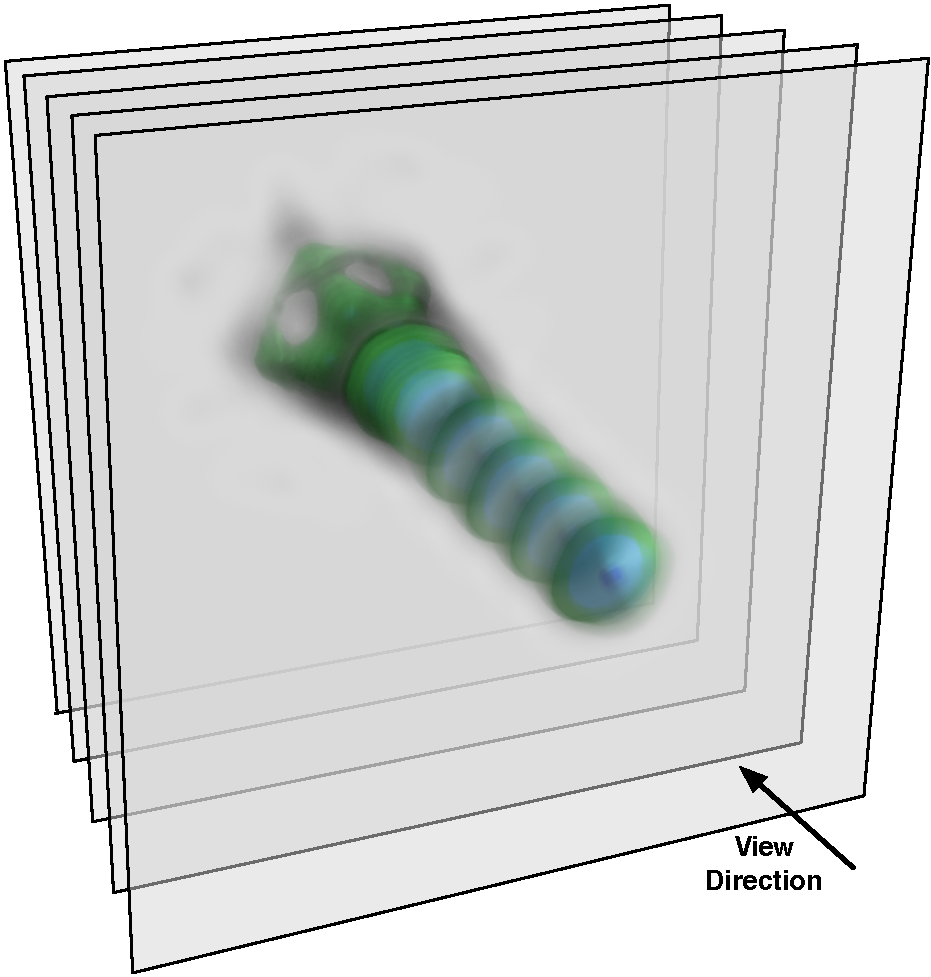
\includegraphics[width=.382\textwidth]{images/slices.pdf}
  {\caption{\small\label{fSlices}Blending Slices in 3D-Texture-based
      Volume Rendering}}
\end{wrapfigure}
 When using 2D (sort-first) or stereo decompositions, no special
programming is needed to achieve good scalability, as \textsf{eVolve} is
mostly fill-limited and therefore scales nicely in these modes. 

The full power of scalable volume rendering is however in DB (sort-last)
compounds, where the full volume is divided into separate bricks. Each
of the bricks is rendered like a separate volume. For recomposition, the
\textsf{RGBA} frame buffer data resulting from these render passes then
has to be assembled correctly. 

Conceptually, the individual volume bricks of each of the source
channels produces pixel data which can be handled like one big 'slice'
through the full texture. Therefore they have to be blen\-ded
back-to-front in the same way as the slice planes are blended during
rendering.

DB compounds have the advantage of scaling any part of the volume
rendering pipeline: texture and main memory (smaller bricks for each
channel), fill rate (less samples per channel) and IO bandwidth for
time-dependent data (less data per time step and channel). Since the
amount of texture memory needed for each node decreases linearly, they
make it possible to render data sets which are not feasible to
visualize with any other approach.

\begin{wrapfigure}{r}{.382\textwidth}
  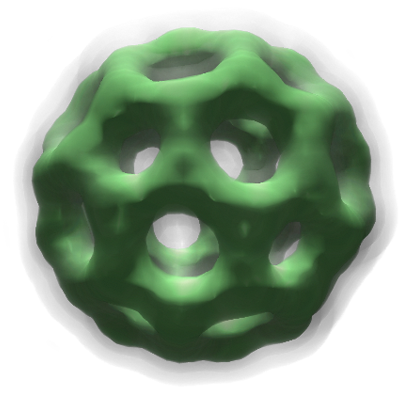
\includegraphics[width=.382\textwidth]{images/volResult.png}
  {\caption{\small\label{fVolResult}Result of \fig{fBlendPerspective}}}
  \vspace{-1em}
\end{wrapfigure}
For recomposition, the 2D frame buffer contents are blended together to
form a seamless picture. For correct blending, the frames are ordered in
the same back-to-front order as the slices used for rendering, and use the
same blending parameters. Simplified, the frame buffer images are
`thick' slices which are `rendered' by writing their content to the
destination frame buffer using the correct order. 

\begin{figure}[h!t]
  \subfigure[]{\label{fBlendOrtho}
    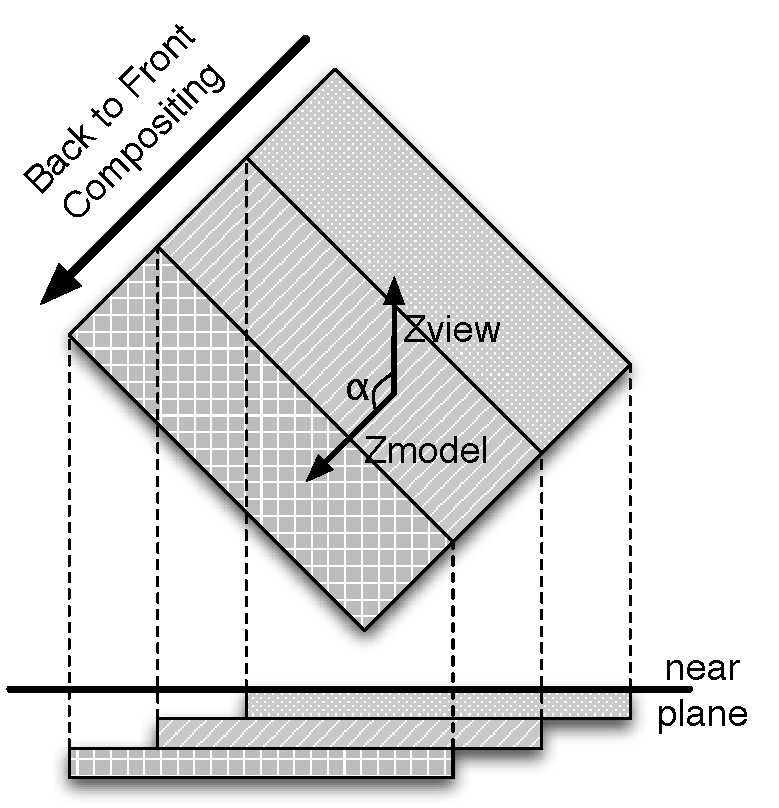
\includegraphics[width=.45\textwidth]{images/b2f_ortho.pdf}
  }\hfil
  \subfigure[]{\label{fBlendPerspective}
    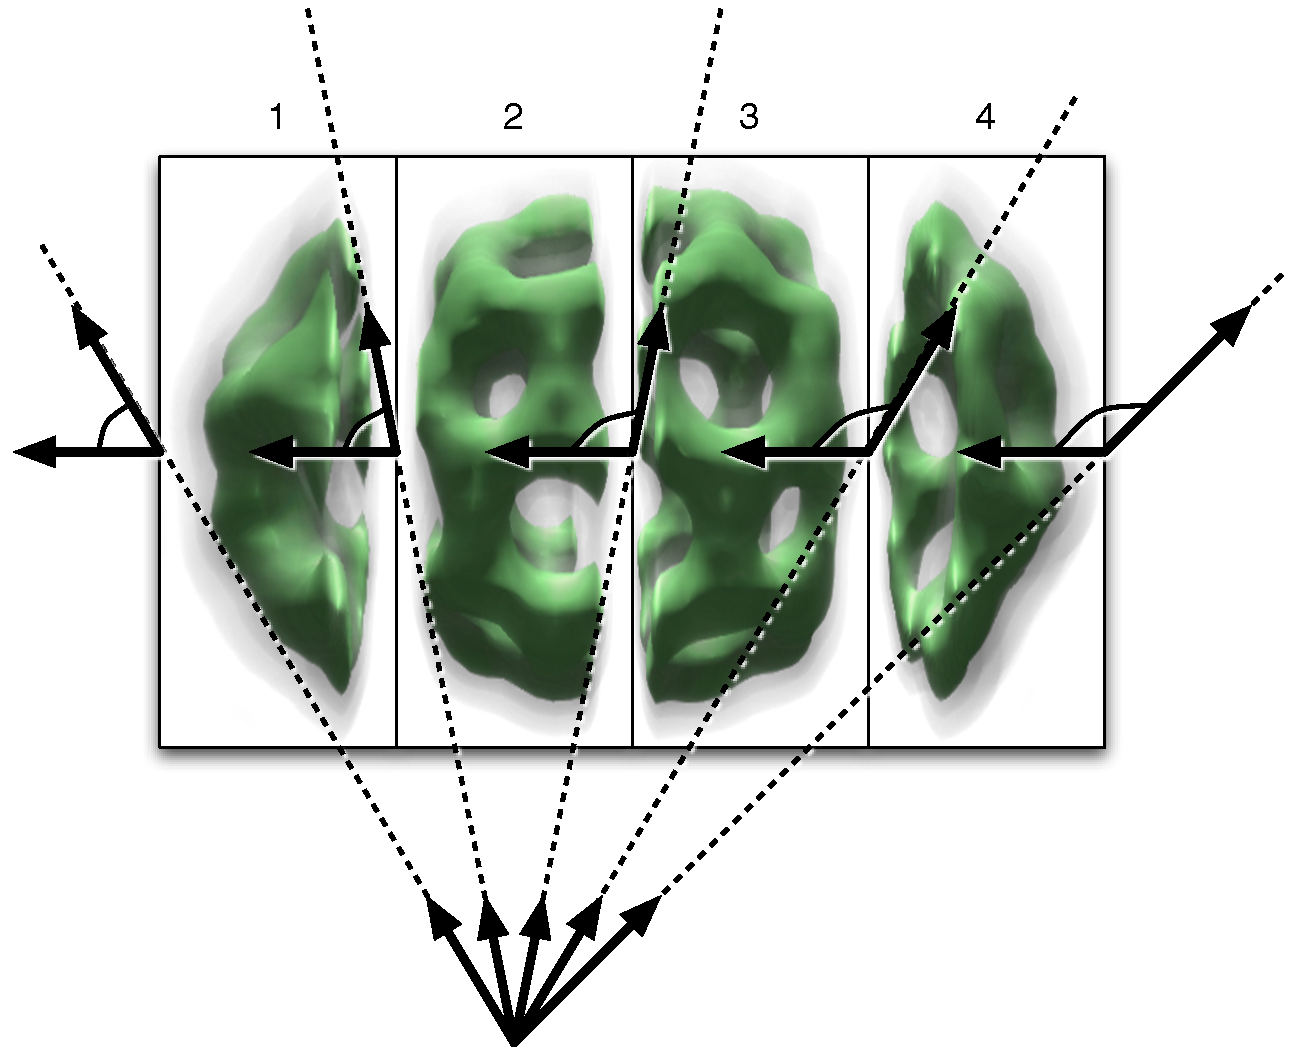
\includegraphics[width=.55\textwidth]{images/b2f_perspective.pdf}
  }%
  {\caption{\small\label{fBlend}Back-to-Front Com\-po\-siting for
      Orthogonal and Perspective View Frustra}}
\end{figure}
For orthographic rendering, determining the compositing order of the
input frames is trivial. The screen-space orientation of the volume
bricks determines the order in which they have to be composited. The
bricks in \textsf{eVolve} are created by slicing the volume along one
dimension. Therefore the range of the resulting frame buffer images,
together with the sorting order, is used to arrange the frames during
compositing. \fig{fBlendOrtho} shows this composition for one view.

Finding the correct assembly order for perspective frustra is more
complex. The perspective distortion invalidates a simple orientation
criteria like the one used for orthographic frustra. For the view and
frustum setup shown in \fig{fBlendPerspective}\footnote{Volume Data Set
  courtesy of: AVS, USA} the correct compositing order is 4-3-1-2 or
1-4-3-2.

In order to compute the assembly order, \textsf{eVolve} uses the angle
between the $origin \rightarrow slice$ vector and the near plane, as shown
in \fig{fBlendPerspective}. When the angle becomes greater than
90\textdegree, the compositing order of the remaining frames has to be
changed. The result image of this composition naturally looks the same
as the volume rendering would when rendered on a single
channel. \fig{fVolResult} shows the result of the composition from
\fig{fBlendPerspective}.

The assembly algorithm described in this section also works with parallel
compositing algorithms such as direct-send. 


\subsection{\label{sStatistics}Statistics}

\subsubsection{Statistics Gathering}

\begin{wrapfigure}{r}{.382\textwidth}
  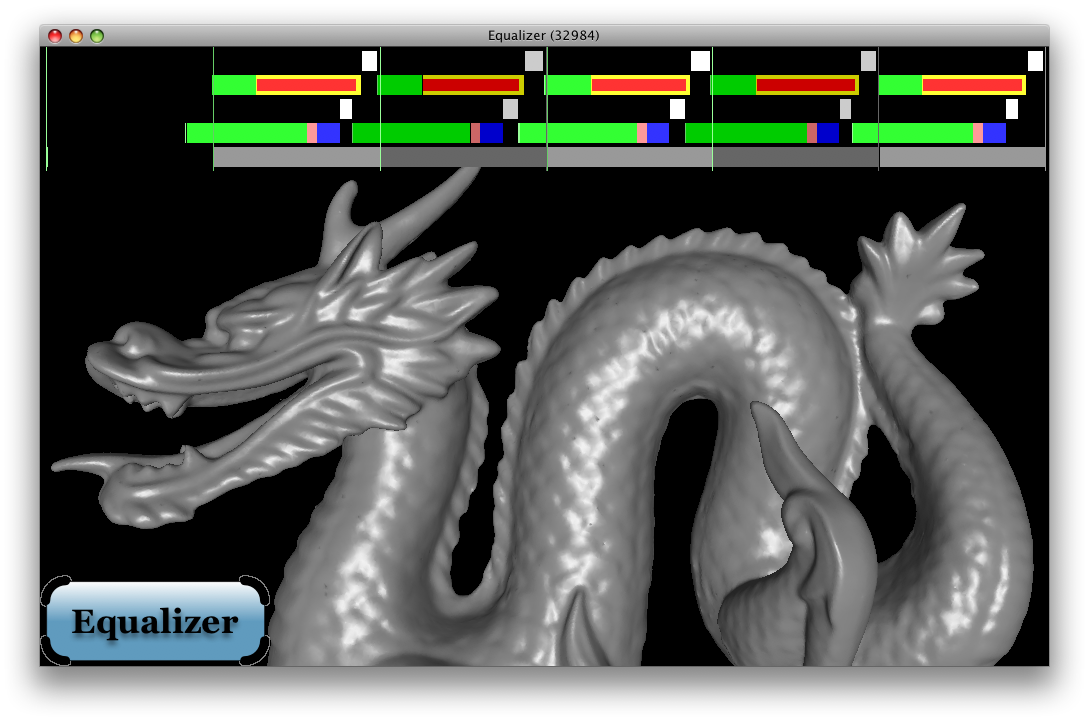
\includegraphics[width=.382\textwidth]{images/statistics.png}
  {\caption{\small\label{fStatistics}Statistics for a two-node 2D compound}}
\end{wrapfigure}
Statistics are measured in milliseconds since the configuration was
initialized. On each node, the global configuration clock is reset at
the same time by the server during \textsf{Config::init}. Each statistic
event records the originator's (channel, window or config) unique
identifier.

Statistics are enabled per entity using an attribute hint. The hint
determines how precise the gathered statistics are. When set to
\textsf{fastest}, the per-frame clock is sampled directly when the event
occurs. When set to \textsf{nicest}, all OpenGL commands will be
finished before sampling the event. This incurs a performance penalty,
but gives more correct results. The default setting is fastest in
release builds, and nicest in debug builds.

The events are processed by the channel's and window's
\textsf{processEvent} method. The default implementation sends these
events to the config, using \textsf{Config::sendEvent}, as explained in
\sref{sEventHandling}. When the default implementation of
\textsf{Config::handleEvent} receives the statistics event, it sorts the
event per frame and per originator. When a frame has been finished, the
events are pushed to the local (app-)node for visualization.

\fig{fStatistics} shows the visualization of statistics events in an
overlay\footnote{3D model courtesy Stanford University Computer Graphics
  Laboratory.}.

\subsubsection{Statistics Overlay}

The Equalizer examples render a statistics overlay using the gathered
statistics events directly before
\textsf{Window::swapBuffers}. Statistics are toggled on and off using
the 's' key. The overlay rendering method,
\textsf{Channel::drawStatistics}, can be called directly by any
application to render the overlay. It can also be overwritten by a
custom implementation.

\begin{figure}[h!t]
  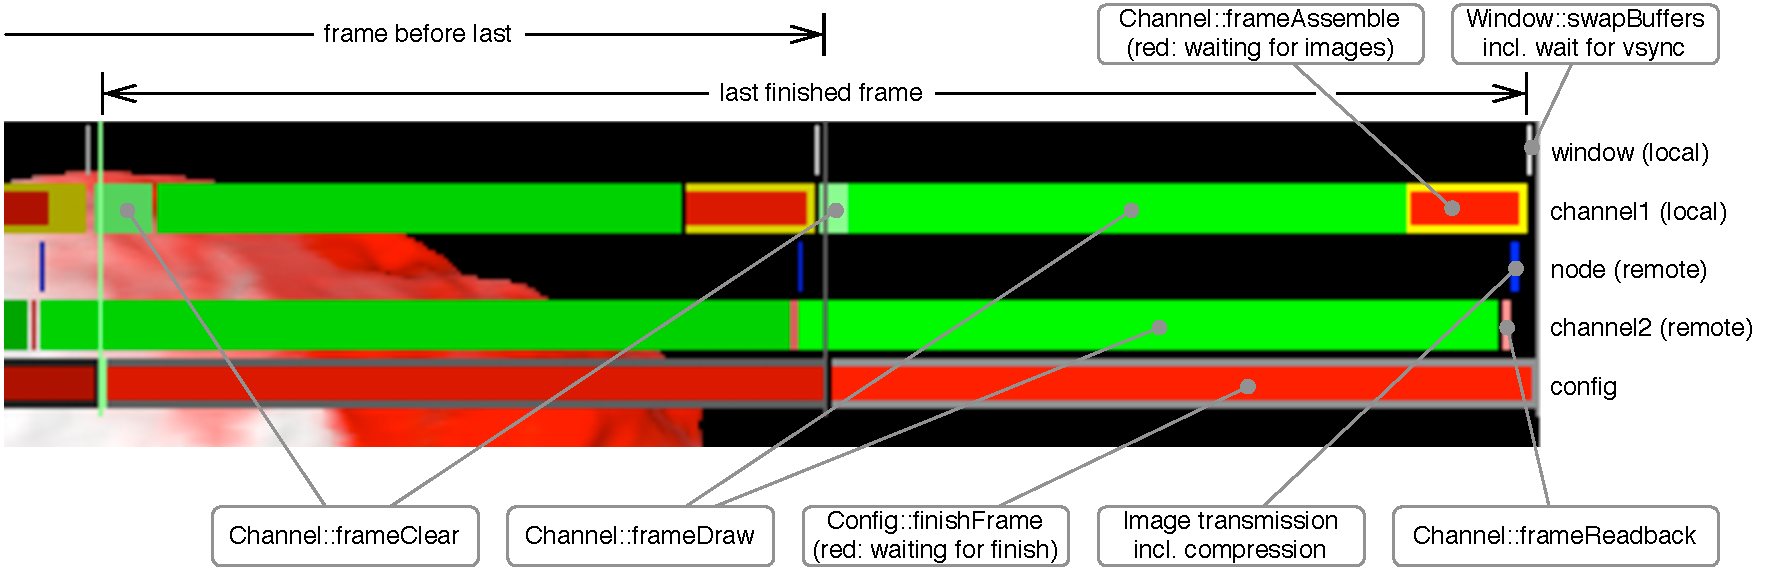
\includegraphics[width=\textwidth]{images/statisticsDetail.pdf}
    {\caption{\small\label{fStatisticsDetail}Annotated Detail of the
        Statistics from \fig{fStatistics}.}}
\end{figure}

\fig{fStatisticsDetail} shows a detail view of \fig{fStatistics},
together with some annotations for the overlay. The statistics shown are
for a two-node 2D compound. The destination channel is on the
\textsf{appNode} and contributes to the rendering.

This compound executes two \textsf{Channel::frameDraw} tasks, one
\textsf{Channel::frame\-Read\-back} task on the remote node and one
\textsf{Channel::frameAssemble} task on the local node.

The X axis is the time. One pixel on the screen corresponds to one
millisecond. The right-most pixel is the most current time. On the Y
axis are the rendering entities: channels, windows and the config. The
upper channel is the local channel since it executes
\textsf{frameAssemble}, and the lower channel is the remote channel,
executing {frameReadback}.

The remote machine is a Mac Mini, the local a MacBook Pro. The draw
times are unbalanced due to the speed difference of the machines, and
the transmit time is relatively long since 100 MBit Ethernet was used.

In order to facilitate the understanding, older frames are gradually
greyed out. The right-most, current frame is brighter than the
frame-before-last.

The configuration used has a latency of one frame. Consequently, the
execution of two frames overlaps. This can be observed in the early
execution of the remote channel's \textsf{frameDraw}, which starts while
the local channel is still assembling the previous frame.

The beginning of a frame is marked by a vertical green line, and the end
of a frame by a vertical gray line. These lines are also attenuated. The
brightness and color matches the event for \textsf{Config::startFrame}
and \textsf{Config::finishFrame}, respectively. The event for
\textsf{startFrame} is typically not visible, since it takes less than
one millisecond to execute. If no idle processing is done by the
application, the event for \textsf{finishFrame} occupies a full frame,
since the config is blocked here waiting for the frame to complete.

In the above example, the local channel finishes drawing the frame
early, and therefore spends a considerable amount of time waiting for
the input frame from the remote channel. These wait events, rendered
red, are a sub-event of the yellow \textsf{frameAssemble} task.

The white \textsf{Window::swapBuffers} task takes also a long time in
debug builds, since the execution of the swap buffer is locked to the
vertical retrace of the display, and enforced by \textsf{glFinish}
before sampling the end time of the event. In release builds, this does
not happen and all OpenGL commands are pipelined with the execution on
the CPU.

The configuration used in this examples does not use a swap
barrier. Swap barrier tasks are solid red events directly in front of
the white swap buffer task.


\newpage
\appendix
\section{\label{aFileFormat}File Format}

The file format currently used is the one-to-one representation of the
server's internal data structures. Its purpose is intermediate, that is,
it will gradually be replaced by automatic resource dedection and
automatic configuration. However the core scalability engine will
always use a similar structure as currently exposed by the file format.

The file format represents an ascii deserialization of the
server. Streaming an \textsf{eq::server::Server} to an \textsf{eq::base::Log}
ostream produces a valid configuration file. Likewise, loading a
configuration file produces an \textsf{eq::server::Server}.

The file format uses the same syntactical structure as VRML. If your
editor supports syntax highlighting and formatting for VRML, you can use
this mode for editing \textsf{.eqc} files.

The configuration file consist of an optional global section and a
server configuration. The global section defines default values for
various attributes. The server section represents an
\textsf{eq::server::Server}.


\subsection{\label{sGlobal}Global Section}

The global section defines default values for attributes used by the
individual entities in the server section. The naming convention for
attributes is:

{\footnotesize\begin{lstlisting}
EQ_<ENTITY>_<DATATYPE>ATTR_<ATTR_NAME>
\end{lstlisting}}

The entity is the capitalized name of the corresponding section later in
the configuration file: connection, config, pipe, window, channel or
compound. The connection is used by the server and nodes.

The datatype is one capital letter for the type of the attribute's
value: \textsf{S} for strings, \textsf{C} for a character, \textsf{I}
for an integer and \textsf{F} for floating-point values. Enumation
values are handled as integers. Strings have always to be surrounded by
double quotes '\textsf{''}'. A character has to be surrounded by single
quotes '\textsf{'}'.

The attribute name is the capitalized name of the entities attribute, as
discussed in the following sections.

Global attribute values have useful default parameters, which can be
overriden with an environment variable of the same name. For enumeration
values the corresponding integer value has to be used. The global values
in the config file override environment variables, and are in turn
overridden by the corresponding attributes sections of the specific
entities.

The globals section starts with the token \textsf{global} and an open
curly brace '\textsf{\{}', and is terminated with a closing curly brace
'\textsf{\}}'. Within the braces, globals are set using the attribute's
name followed by its value. The following attributes are available:

\begin{center}
\begin{tabularx}{\textwidth}{|l|X|}
  \hline
  \textbf{Name} & EQ\_CONNECTION\_SATTR\_HOSTNAME\\
  \textbf{Value} & string\\
  \textbf{Default} & ''localhost''\\
  \textbf{Details} & The hostname or IP address used to connect the
  server or node. When used for the server, the listening port of the
  server is bound to this address. When used for a node, the server
  first tries to connect to the render client node using this hostname,
  and then tries to launch the render client executable on this host.\\
  \hline
\end{tabularx}\\\vfill

\begin{tabularx}{\textwidth}{|l|X|}
  \hline
  \textbf{Name} & EQ\_CONNECTION\_SATTR\_LAUNCH\_COMMAND\\
  \textbf{Value} & string\\
  \textbf{Default} & ssh -n \%h \%c \textgreater\& \%h.\%n.log [POSIX]\\
                   & ssh -n \%h \%c [WIN32]\\
  \textbf{Details} & The command used by the server to launch nodes
  which could not be connected. The launch command is executed from a
  process forked from the server process. The \% tokens are replaced by
  the server at runtime with concrete data: \%h is replaced by the
  hostname, \%c by the command to launch, including command line
  arguments and \%n by a node-unique identifier. Each command line
  argument is surrounded by launch command quotes.\\
  \hline
\end{tabularx}\\\vfill

\begin{tabularx}{\textwidth}{|l|X|}
  \hline
  \textbf{Name} & EQ\_CONNECTION\_CATTR\_LAUNCH\_COMMAND\_QUOTE\\
  \textbf{Value} & character\\
  \textbf{Default} & ' [POSIX]\\
                   & '' [WIN32]\\
  \textbf{Details} & The server uses command line arguments to launch
  render client nodes correctly. Certain launch commands or shells use
  different conventions to separate command line arguments. These
  arguments might contain white spaces, and therefore have to be
  surrounded by quotes to
  identify their borders.\\
  \hline
\end{tabularx}\\\vfill

\begin{tabularx}{\textwidth}{|l|X|}
  \hline
  \textbf{Name} & EQ\_CONNECTION\_IATTR\_TYPE\\
  \textbf{Value} & TCPIP \textbar \ SDP\\
  \textbf{Default} & TCPIP\\
  \textbf{Details} & The protocol for connections. SDP
  programmatically selects the socket direct protocol (AF\_INET\_SDP)
  provided by most InfiniBand protocol stacks, TCPIP uses normal TCP
  sockets (AF\_INET).\\
  \hline
\end{tabularx}\\\vfill

\begin{tabularx}{\textwidth}{|l|X|}
  \hline
  \textbf{Name} & EQ\_CONNECTION\_IATTR\_TCPIP\_PORT\\
  \textbf{Value} & unsigned\\
  \textbf{Default} & 0\\
  \textbf{Details} & The listening port used by the server or
  node. For nodes, the port can be used to contact pre-started, resident
  render client nodes or to use a specific port for the node. If 0 is
  specified, a random port is chosen. Note that a server with no
  connections automatically creates a default connection using the
  server's default port.\\
  \hline
\end{tabularx}\\\vfill

\begin{tabularx}{\textwidth}{|l|X|}
  \hline
  \textbf{Name} & EQ\_CONNECTION\_IATTR\_LAUNCH\_TIMEOUT\\
  \textbf{Value} & unsigned\\
  \textbf{Default} & 60'000\\
  \textbf{Details} & Defines the timeout in milliseconds to wait for
  an auto-launched node. If the render client process did not contact
  the server within that time, the node is considered to be unreachable
  and the initialization of the configuration fails.\\
  \hline
\end{tabularx}\\\vfill

\begin{tabularx}{\textwidth}{|l|X|}
  \hline
  \textbf{Name} & EQ\_CONFIG\_FATTR\_EYE\_BASE\\
  \textbf{Value} & float\\
  \textbf{Default} & 0.05\\
  \textbf{Details} & The distance in meters between the left and the
  right eye, i.e., the eye separation. The eye base influences the
  frustum during stereo rendering. See \sref{sTracking} for details.\\
  \hline
\end{tabularx}\\\vfill

\begin{tabularx}{\textwidth}{|l|X|}
  \hline
  \textbf{Name} & EQ\_PIPE\_IATTR\_HINT\_THREAD\\
  \textbf{Value} & OFF \textbar \ ON\\
  \textbf{Default} & ON\\
  \textbf{Details} & Determines if all task methods for a pipe and its
  children are executed from a separate operating system thread
  (default) or from the node main thread. Non-threaded pipes have
  certain performance limitations and should only be used where necessary.\\
  \hline
\end{tabularx}\\\vfill

\begin{tabularx}{\textwidth}{|l|X|}
  \hline
  \textbf{Name} & EQ\_WINDOW\_IATTR\_HINT\_STEREO\\
  \textbf{Value} & OFF \textbar \ ON \textbar \ AUTO\\
  \textbf{Default} & AUTO\\
  \textbf{Details} & Determines if the window selects a quad-buffered
  stereo visual. When set to AUTO, the window initialization methods try
  to allocate a stereo visual for windows, but fall back to a mono
  visual if allocation fails. For PBuffers, AUTO selects a mono visual.\\
  \hline
\end{tabularx}\\\vfill

\begin{tabularx}{\textwidth}{|l|X|}
  \hline
  \textbf{Name} & EQ\_WINDOW\_IATTR\_HINT\_DOUBLEBUFFER\\
  \textbf{Value} & OFF \textbar \ ON \textbar \ AUTO\\
  \textbf{Default} & AUTO\\
  \textbf{Details} & Determines if the window selects a double-buffered
  stereo visual. When set to AUTO, the window initialization methods try
  to allocate a double-buffered visual for windows, but fall back to a
  single-buffered visual if allocation fails. For PBuffers, AUTO selects
  a single-buffered visual.\\
  \hline
\end{tabularx}\\\vfill

\begin{tabularx}{\textwidth}{|l|X|}
  \hline
  \textbf{Name} & EQ\_WINDOW\_IATTR\_HINT\_DECORATION\\
  \textbf{Value} & OFF \textbar \ ON\\
  \textbf{Default} & ON\\
  \textbf{Details} & When set to OFF, window borders and other
  decorations are disabled, and typically the window can not be moved or
  resized. This option is useful for source windows during
  decomposition. The implementation is window-system specific.\\
  \hline
\end{tabularx}\\\vfill

\begin{tabularx}{\textwidth}{|l|X|}
  \hline
  \textbf{Name} & EQ\_WINDOW\_IATTR\_HINT\_FULLSCREEN\\
  \textbf{Value} & OFF \textbar \ ON\\
  \textbf{Default} & OFF\\
  \textbf{Details} & When set to ON, the window displays in
  fullscreen. This option forces window decorations to be OFF. The
  implementation is window-system specific.\\
  \hline
\end{tabularx}\\\vfill

\begin{tabularx}{\textwidth}{|l|X|}
  \hline
  \textbf{Name} & EQ\_WINDOW\_IATTR\_HINT\_SWAPSYNC\\
  \textbf{Value} & OFF \textbar \ ON\\
  \textbf{Default} & ON\\
  \textbf{Details} & Determines if the buffer swap is synchronized with
  the vertical retrace of the display. This option is currently not
  implemented for GLX. For WGL, the WGL\_EXT\_swap\_control extension is
  required. For optimal performance, set swap synchronization to OFF for
  source-only windows.\\
  \hline
\end{tabularx}\\\vfill

\begin{tabularx}{\textwidth}{|l|X|}
  \hline
  \textbf{Name} & EQ\_WINDOW\_IATTR\_HINT\_DRAWABLE\\
  \textbf{Value} & window \textbar \ pbuffer\\
  \textbf{Default} & window\\
  \textbf{Details} & Selects the window's drawable type. A window is an
  on-screen, window system-dependent window with a full-window OpenGL
  drawable. PBuffers are off-screen drawables created using window
  system-dependent PBuffer API's. In order to calculate the PBuffer size
  on unconnected devices, a pipe viewport size of 4096x4096 is assumed,
  unless specified otherwise.\\
  \hline
\end{tabularx}\\\vfill

\begin{tabularx}{\textwidth}{|l|X|}
  \hline
  \textbf{Name} & EQ\_WINDOW\_IATTR\_HINT\_STATISTICS\\
  \textbf{Value} & OFF \textbar \ FASTEST [ON] \textbar \ NICEST\\
  \textbf{Default} & FASTEST [Release Build]\\
                   & NICEST [Debug Build]\\
  \textbf{Details} & Determines how statistics are gathered. OpenGL
  buffers commands, which causes the rendering to be executed at an
  arbitrary point in time. Nicest statistics gathering executes a
  \textsf{Window::finish}, which calls by default \textsf{glFinish}, in
  order to accurately account the rendering operations to the sampled
  task method. However, calling \textsf{glFinish} has a performance
  impact. Therefore, the fastest statistics gathering samples the task
  statistics directly, without finishing the OpenGL commands first. Some
  operations, e.g., frame buffer readback, inherently finish all
  previous OpenGL commands.\\
  \hline
\end{tabularx}\\\vfill

\begin{tabularx}{\textwidth}{|l|X|}
  \hline
  \textbf{Name} & EQ\_WINDOW\_IATTR\_PLANES\_COLOR\\
  \textbf{Value} & unsigned\\
  \textbf{Default} & AUTO\\
  \textbf{Details} & Determines the number of color planes for the
  window. The interpretation of this value is window system-specific, as
  some window systems select a visual with the closest match to this
  value, and some select a visual with at least the number of color
  planes specified. AUTO selects a visual with a reasonable quality,
  typically eight bits per color.\\
  \hline
\end{tabularx}\\\vfill

\begin{tabularx}{\textwidth}{|l|X|}
  \hline
  \textbf{Name} & EQ\_WINDOW\_IATTR\_PLANES\_ALPHA\\
  \textbf{Value} & unsigned\\
  \textbf{Default} & UNDEFINED\\
  \textbf{Details} & Determines the number of alpha planes for the
  window. The interpretation of this value is window system-specific, as
  some window systems select a visual with the closest match to this
  value, and some select a visual with at least the number of alpha
  planes specified. By default no alpha planes are requested.\\
  \hline
\end{tabularx}\\\vfill

\begin{tabularx}{\textwidth}{|l|X|}
  \hline
  \textbf{Name} & EQ\_WINDOW\_IATTR\_PLANES\_DEPTH\\
  \textbf{Value} & unsigned\\
  \textbf{Default} & AUTO\\
  \textbf{Details} & Determines the precision of the depth buffer. The
  interpretation of this value is window system-specific, as some window
  systems select a visual with the closest match to this value, and some
  select a visual with at least the number of depth bits specified. AUTO
  select a visual with a reasonable depth precision, typically 24 bits.\\
  \hline
\end{tabularx}\\\vfill

\begin{tabularx}{\textwidth}{|l|X|}
  \hline
  \textbf{Name} & EQ\_WINDOW\_IATTR\_PLANES\_STENCIL\\
  \textbf{Value} & unsigned\\
  \textbf{Default} & AUTO\\
  \textbf{Details} & Determines the number of stencil planes for the
  window. The interpretation of this value is window system-specific, as
  some window systems select a visual with the closest match to this
  value, and some select a visual with at least the number of stencil
  planes specified. AUTO tries to select a visual with at least one
  stencil plane, but falls back to no stencil planes if allocation
  fails. Note that for depth-compositing and pixel-compositing at least
  one stencil plane is needed.\\
  \hline
\end{tabularx}\\\vfill

\begin{tabularx}{\textwidth}{|l|X|}
  \hline
  \textbf{Name} & EQ\_WINDOW\_IATTR\_PLANES\_ACCUM\\
  \textbf{Value} & unsigned\\
  \textbf{Default} & UNDEFINED\\
  \textbf{Details} & Determines the number of color accumulation buffer
  planes for the window. The interpretation of this value is window
  system-specific, as some window systems select a visual with the
  closest match to this value, and some select a visual with at least
  the number of accumulation buffer planes specified.\\
  \hline
\end{tabularx}\\\vfill

\begin{tabularx}{\textwidth}{|l|X|}
  \hline
  \textbf{Name} & EQ\_WINDOW\_IATTR\_PLANES\_ACCUM\_ALPHA\\
  \textbf{Value} & unsigned\\
  \textbf{Default} & UNDEFINED\\
  \textbf{Details} & Determines the number of alpha accumulation buffer
  planes for the window. The interpretation of this value is window
  system-specific, as some window systems select a visual with the
  closest match to this value, and some select a visual with at least
  the number of accumulation buffer planes specified. If this attribute
  is undefined, the value of EQ\_WINDOW\_IATTR\_PLANES\_ACCUM is used to
  determine the number of alpha accumulation buffer planes.\\
  \hline
\end{tabularx}\\\vfill

\begin{tabularx}{\textwidth}{|l|X|}
  \hline
  \textbf{Name} & EQ\_WINDOW\_IATTR\_PLANES\_SAMPLES\\
  \textbf{Value} & unsigned\\
  \textbf{Default} & UNDEFINED\\
  \textbf{Details} & Determines the number of samples used for multisampling.\\
  \hline
\end{tabularx}\\\vfill

\begin{tabularx}{\textwidth}{|l|X|}
  \hline
  \textbf{Name} & EQ\_CHANNEL\_IATTR\_HINT\_STATISTICS\\
  \textbf{Value} & OFF \textbar \ FASTEST [ ON ] \textbar \ NICEST\\
  \textbf{Default} & FASTEST [Release Build]\\
                   & NICEST [Debug Build]\\
  \textbf{Details} & See EQ\_WINDOW\_IATTR\_HINT\_STATISTICS.\\
  \hline
\end{tabularx}\\\vfill

\begin{tabularx}{\textwidth}{|l|X|}
  \hline
  \textbf{Name} & EQ\_COMPOUND\_IATTR\_STEREO\_MODE\\
  \textbf{Value} & QUAD \textbar \ ANAGLYPH\\
  \textbf{Default} & QUAD\\
  \textbf{Details} & Selects the algorithm used for stereo
  rendering. QUAD-buffered stereo uses the left and right buffers of a
  stereo window (active stereo). Anaglyphics stereo uses
  \textsf{glColorMask} to mask colors for individual eye passes, used in
  conjunction with colored glasses.\\
  \hline
\end{tabularx}\\\vfill

\begin{tabularx}{\textwidth}{|l|X|}
  \hline
  \textbf{Name} & EQ\_COMPOUND\_IATTR\_STEREO\_ANAGLYPH\_LEFT\_MASK\\
  \textbf{Value} & [ RED GREEN BLUE ]\\
  \textbf{Default} & [ RED ] \\
  \textbf{Details} & Select the color mask for the left eye pass during
  anaglyphic stereo rendering.\\
  \hline
\end{tabularx}\\\vfill

\begin{tabularx}{\textwidth}{|l|X|}
  \hline
  \textbf{Name} & EQ\_COMPOUND\_IATTR\_STEREO\_ANAGLYPH\_RIGHT\_MASK\\
  \textbf{Value} & [ RED GREEN BLUE ]\\
  \textbf{Default} & [ GREEN BLUE ]\\
  \textbf{Details} & Select the color mask for the right eye pass during
  anaglyphic stereo rendering.\\
  \hline
\end{tabularx}\\\vfill

\begin{tabularx}{\textwidth}{|l|X|}
  \hline
  \textbf{Name} & EQ\_COMPOUND\_IATTR\_UPDATE\_FOV\\
  \textbf{Value} & HORIZONTAL [ON] \textbar \ VERTICAL \textbar \ OFF\\
  \textbf{Default} & HORIZONTAL\\
  \textbf{Details} & Define how the wall or projection description is
  updated when a window is resized. Horizontal increases or decreases
  the horizontal field of view, while keeping the vertical size
  constant. Vertical updates the vertical field of view, while keeping
  the horizontal size constant. OFF does not update the wall or
  projection description at all.\\
  \hline
\end{tabularx}\\
\end{center}

\subsection{Server Section}

The server section consists of connection description parameters for the
server listening sockets, and a number of configurations for this
server. Currently only the first configuration is used.

\subsubsection{\label{sConnectionDescription}Connection Description}

A connection description defines the network parameters of an Equalizer
process. Currently two connection types, TCP/IP and SDP, are
supported. TCP/IP creates a TCP socket. SDP is very similar, except that
the address family \textsf{AF\_INET\_SDP} instead of \textsf{AF\_INET}
is used to enforce a SDP connection. Note that you can also use the
transparent mode provided by most InfiniBand implementations to used SDP
with TCP connections. 

Furthermore, a port for the socket can be specified. When no port is
specified for the server, the default port 4242 (+UID on Posix systems)
is used. When no port is specified for a node, a random port will be
chosen by the operating system. For pre-launched render clients, a port
has to be specified for the server to find the client node.

The hostname is the IP address or (resolvable) host name. When used for
the server, the server binds its listening socket only to the specified
name.

A server or node may have multiple connection descriptions. A server
binds to all provided connection descriptions. For a node, all
connection descriptions are used while trying to establish a connection
to the node. When auto-launched by the server, all connection
descriptions are passed to the launched node process, which binds to all
provided descriptions.

{\footnotesize\begin{lstlisting}
server
{
    connection // 0-n times, listening connections of the server
    {
        type       TCPIP | SDP
        TCPIP_port unsigned
        hostname   string
    }

    config {...} // 1-n times, currently only the first one is used by the server
}
\end{lstlisting}}

\subsubsection{Config Section}

A configuration has a number of parameters, nodes and compounds.

The nodes and their children describe the rendering resources in a
natural, hierarchical way. Compounds use rendering resources (channels)
to execute rendering tasks. For an introduction on the concepts of
nodes, pipes, windows, channels and compounds please refer to
\sref{sConfig} and \sref{sCompounds}.

The latency of a config defines the maximum number of frames the
slowest operation may fall behind the application thread. A latency of 0
synchronizes all rendering tasks started by \textsf{Config::startFrame}
in \textsf{Config::finishFrame}. A latency of one synchronizes all
rendering tasks started one frame ago in \textsf{finishFrame}.

For a description of config attributes please refer to \sref{sGlobal}.

{\footnotesize\begin{lstlisting}
config
{
    latency int    // # of frames nodes may fall behind application
    attributes
    {
         eye_base float // distance between left and right eye
    }

    (node|appNode) {...}// 1-n times, a system in the cluster
                   // 0|1 appNode: launches render thread within app process
    compound {...} // 1-n times
}
\end{lstlisting}}

\subsubsection{Node Section}

A node represents a machine in the cluster, and is one process. It has a
name, a number of connection descriptions and at least one pipe. The
name of the node can be used for debugging, it has no influence on the
execution of Equalizer. For a description of connection attributes
please refer to \sref{sGlobal}.

{\footnotesize\begin{lstlisting}
node
{
    name     string
    connection // 0-n times, possible connections to this node
    {
        type          TCPIP | SDP
        TCPIP_port    unsigned
        hostname      string
        command       string      // render client launch command
        command_quote 'character' // launch command argument quote char
        timeout       unsigned    // timeout in milliseconds for launch
    }
    pipe {...} // 1-n times
}
\end{lstlisting}}

\subsubsection{Pipe Section}

A pipe represents a graphics card (GPU), and is one execution thread. It
has a name, GPU settings and attributes. The name of a pipe can be used
for debugging, it has no influence on the execution of Equalizer.

The GPU is identified by two parameters, a port and a device. The port
is only used for the GLX window system, and identifies the port number
of the X server, i.e., the number after the colon in the DISPLAY
description (':\textbf{0}.1').

The device identifies the graphics adapter. For the GLX window system
this is the screen number, i.e., the number after the dot in the DISPLAY
description (:0.\textbf{1}). The OpenGL output is always restricted by
glX to the GPU attached to selected screen.

For the AGL window system, the device selects the \textit{n}th display
in the list of online displays. The OpenGL output is optimized for the
selected display, but not restricted to the attached GPU.

For the WGL window system, the device selects the \textit{n}th GPU in
the system. The GPU can be offline, in this case only PBuffer windows
can be used. In order to restrict the OpenGL output to the GPU, the
\textsf{WGL\_NV\_gpu\_affinity} extension is used. If the extension is
not present, the window is opened on the \textit{n}th monitor, but
OpenGL commands are sent to all GPU's.

The viewport of the pipe can be used to override the pipe
resolution. The viewport is defined in pixels. The x and y parameter of
the viewport are currently ignored. The default viewport is
automatically detected. For offline GPU's, a default of 4096x4096 is
used.

For a description of pipe attributes please refer to \sref{sGlobal}.

{\footnotesize\begin{lstlisting}
pipe
{
    name     string
    port     unsigned     // X server number or ignored
    device   unsigned     // graphics adapter number
    viewport [ viewport ] // default: autodetect
    attributes
    {
        hint_thread   OFF | ON   // default ON
    }

    window {...} // 1-n times
}
\end{lstlisting}}

\subsubsection{Window Section}

A window represents an OpenGL drawable and holds an OpenGL context. It
has a name, a viewport and attributes. The name of a window can be used
for debugging, it has no influence on the execution of Equalizer.

The viewport of the window is relative to the pipe. It can be specified
in relative or absolute coordinates. Relative coordinates are normalized
coordinates with respect to the pipe, e.g., a viewport of \textsf{[ 0.25
  0.25 0.5 0.5 ]} creates a window in the middle of the screen, using
50\% of the pipe's size. Absolute coordinates are integer pixel values,
e.g., a viewport of \textsf{[ 50 50 800 600 ]} creates a window 50 pixels
from the upper-left corner, sized 800x600 pixels, regardless of the
pipe's size. The default viewport is \textsf{[ 0 0 1 1 ]}, i.e., a
full-screen window. 

For a description of window attributes please refer to \sref{sGlobal}.

{\footnotesize\begin{lstlisting}
window
{
    name     string
    viewport [ viewport ] // wrt pipe, default full screen

    attributes
    {
        hint_stereo         OFF | ON | AUTO
        hint_doublebuffer   OFF | ON | AUTO
        hint_decoration     OFF | ON
        hint_fullscreen     OFF | ON
        hint_swapsync       OFF | ON         // AGL, WGL only
        hint_drawable       window | pbuffer
        hint_statistics     off | fastest [on] | nicest
        planes_color        unsigned
        planes_alpha        unsigned
        planes_depth        unsigned
        planes_stencil      unsigned
        planes_accum        unsigned
        planes_accum_alpha  unsigned
        planes_samples      unsigned
    }

    channel {...} // 1-n times
}
\end{lstlisting}}

\subsubsection{Channel Section}

A channel is a two-dimensional area within a window. It has a name,
viewport and attributes. The name of the channel is used to identify the
channel in the respective compounds. It should be unique within the config.

The viewport of the channel is relative to the window. As for windows,
it can be specified in relative or absolute coordinates. The default
viewport is \textsf{[ 0 0 1 1 ]}, i.e., fully covering its window.

For a description of channel attributes please refer to \sref{sGlobal}.

{\footnotesize\begin{lstlisting}
channel
{
    name     string
    viewport [ viewport ] //wrt window, default full window

    attributes
    {
        hint_statistics     OFF | FASTEST [ON] | NICEST
    }
}
\end{lstlisting}}

\subsubsection{Compound Section}

Compounds are the basic datastructure describing the rendering
setup. They use channels for rendering. Please refer to
\sref{sCompounds} for a description of compound operation logics.

The name of the compound is used for the default names of swap barriers
and output frames. The channel references the first channel of the same
name in the configuration.

Compound tasks describe the operations the compound executes. The
default is all tasks for compounds with no children (leaf compounds) and
\textsf{READBACK ASSEMBLE} for all others. The readback and assemble
tasks are only executed if the compound has output frames or input
frames, respectively. Tasks are not inherited by the children of a
compound.

The buffer defines the default frame buffer attachments read back by
output frames. The viewport restricts the rendering to the area relative
to the parent compound. The range restricts the database range, relative
to the parent. The pixel setting selects the pixel decomposition
parameters, relative to the parent. The eye pass select the mono, left
or right eye passes rendered by the compound. All these attributes are
inherited by the children of a compound. Viewport, range and pixel
parameters are cumulative.

For a description of compound attributes please refer to \sref{sGlobal}.

A wall or projection description is used to define the view frustum of
the compound. The frustum is inherited and typically only defined on the
top-most compound. The last specified frustum description is used. Sizes
are specified in meters. \fig{fFrustra} illustrates the frustum
parameters.

A swap barrier is used to synchronize the output of multiple
compounds. All swap barriers of the same name are synchronized The
default name is \textsf{barrier[.root\-Com\-pound\-Name]}.

Output frames transport frame buffer contents to input frames of the
same name. If the compound has a name, the default frame name is
\textsf{frame.compoundName}, otherwise the default name is
\textsf{frame.channelName}. The frame buffer attachments to read back
are inherited from the compound, but can be overridden by output frames.

{\footnotesize\begin{lstlisting}
compound
{
    name     string
    channel  string   // where the compound's tasks are executed
    task     [ CLEAR DRAW READBACK ASSEMBLE ] // CULL later
    buffer   [ COLOR DEPTH ]         // default COLOR
    viewport [ viewport ]            // wrt parent compound, sort-first
    range    [ float float ]         // DB-range for sort-last
    pixel    [ int int ]             // pixel decomposition (step size)
    eye      [ CYCLOP LEFT RIGHT ]   // monoscopic or stereo view
    attributes
    {
        stereo_mode                  QUAD | ANAGLYPH    // default QUAD
        stereo_anaglyph_left_mask    [ RED GREEN BLUE ] // default red
        stereo_anaglyph_right_mask   [ RED GREEN BLUE ] // df green blue
        update_FOV                   HORIZONTAL [ON] | VERTICAL | OFF
    }

    wall       // frustum description
    {
        bottom_left  [ float float float ]
        bottom_right [ float float float ]
        top_left     [ float float float ]
    }
    projection // alternate frustum description, last one wins
    {
        origin       [ float float float ]
        distance     float
        fov          [ float float ]
        hpr          [ float float float ]
    }
    
    child-compounds

    swapbarrier  // compounds with the same barriername sync swap
    {
        name string
    }
    outputframe
    {
        name   string
        buffer [ COLOR DEPTH ]
    }
    inputframe
    {
        name string // corresponding output frame
    }
}
\end{lstlisting}}

\if 0
{\footnotesize\begin{lstlisting}
\end{lstlisting}}
\fi

\end{document}
